% =============================================================================
%  Formal Genetics: Proof, Computation and Evidence in Molecular Biology
%  A student textbook in twelve sections.
%
%  Each section lives in its own file under sections/ and builds independently
%  (see build.py --section N), so a section can be written, compiled and
%  reviewed without touching the others.
% =============================================================================
\documentclass[11pt,a4paper]{article}

\usepackage{cmap}
\usepackage[T1]{fontenc}
\usepackage[utf8]{inputenc}
\usepackage{lmodern}
\usepackage{microtype}
\usepackage{amsmath,amssymb,amsthm,mathtools}
\usepackage{booktabs,tabularx,array,longtable}
\usepackage{graphicx}
\usepackage{caption,subcaption}
\usepackage{xcolor}
\usepackage{listings}
\usepackage{enumitem}
\usepackage{siunitx}
\usepackage[most]{tcolorbox}
\usepackage[hidelinks]{hyperref}

\graphicspath{{figures/}{../figures/}}

% This book is dense with long identifiers (gene symbols, Lean names, paths).
% Let TeX stretch a difficult paragraph rather than let a line overflow the
% measure; `build.py` treats any remaining overfull box as a build failure.
\setlength{\emergencystretch}{3em}

% ---------------------------------------------------------------- colours ---
\definecolor{inkblue}{HTML}{14365C}
\definecolor{proofgreen}{HTML}{1B7A52}
\definecolor{datawarm}{HTML}{B4521E}
\definecolor{softgrey}{HTML}{F4F4F2}
\definecolor{rulegrey}{HTML}{8A8A86}
\definecolor{leanpurple}{HTML}{5B3E8E}

% ------------------------------------------------------- theorem machinery ---
\theoremstyle{plain}
\newtheorem{theorem}{Theorem}[section]
\newtheorem{lemma}[theorem]{Lemma}
\newtheorem{proposition}[theorem]{Proposition}
\newtheorem{corollary}[theorem]{Corollary}
\theoremstyle{definition}
\newtheorem{definition}[theorem]{Definition}
\newtheorem{model}[theorem]{Modelling Assumption}
\theoremstyle{remark}
\newtheorem{remark}[theorem]{Remark}

% --------------------------------------------------------- student blocks ---
% Learning objectives, opening every section.
\newtcolorbox{objectives}{
  enhanced, breakable, colback=softgrey, colframe=inkblue,
  boxrule=0.4pt, left=8pt, right=8pt, top=6pt, bottom=6pt, arc=2pt,
  title=\textbf{What you should be able to do after this section},
  fonttitle=\small\bfseries, coltitle=white, colbacktitle=inkblue}

% A fully worked example the student can follow line by line.
\newtcolorbox{worked}[1][]{
  enhanced, breakable, colback=white, colframe=proofgreen,
  boxrule=0.5pt, left=8pt, right=8pt, top=6pt, bottom=6pt, arc=2pt,
  title={Worked Example#1}, fonttitle=\small\bfseries,
  coltitle=white, colbacktitle=proofgreen}

% The epistemic ledger: the distinctive device of this book. Every section ends
% with one, separating what is measured from what is assumed from what is proved.
% The optional argument replaces the title, for the one case where the box
% carries a section's controls rather than its ledger. Existing uses with no
% argument keep the default title.
\newtcolorbox{ledger}[1][Epistemic ledger for this section]{
  enhanced, breakable, colback=white, colframe=rulegrey,
  boxrule=0.5pt, left=8pt, right=8pt, top=6pt, bottom=6pt, arc=2pt,
  title={\textbf{#1}},
  fonttitle=\small\bfseries, coltitle=white, colbacktitle=rulegrey}

% Numerical result reproduced from a named script.
\newtcolorbox{numerics}[1][]{
  enhanced, breakable, colback=white, colframe=datawarm,
  boxrule=0.5pt, left=8pt, right=8pt, top=6pt, bottom=6pt, arc=2pt,
  title={Numerical resolution#1}, fonttitle=\small\bfseries,
  coltitle=white, colbacktitle=datawarm}

\newcounter{exercisectr}[section]
\newenvironment{exercise}[1][]
  {\refstepcounter{exercisectr}\par\medskip\noindent
   \textbf{Exercise \thesection.\theexercisectr}\ #1\par\nobreak\smallskip}
  {\par\medskip}

% ------------------------------------------------------------ Lean listing ---
\lstdefinestyle{lean}{
  basicstyle=\ttfamily\footnotesize,
  keywordstyle=\color{leanpurple}\bfseries,
  commentstyle=\color{rulegrey}\itshape,
  stringstyle=\color{datawarm},
  showstringspaces=false, breaklines=true, frame=single,
  rulecolor=\color{rulegrey}, framesep=5pt, xleftmargin=6pt,
  morekeywords={theorem,lemma,def,noncomputable,open,namespace,end,import,by,
    intro,exact,apply,have,show,calc,simp,norm_num,linarith,nlinarith,unfold,
    rcases,refine,fun,let,if,then,else,Finset,Real,Prop,Type},
  literate={≤}{{$\leq$}}1 {≥}{{$\geq$}}1 {∈}{{$\in$}}1 {⊆}{{$\subseteq$}}1
           {∀}{{$\forall$}}1 {∃}{{$\exists$}}1 {∏}{{$\prod$}}1 {∑}{{$\sum$}}1
           {→}{{$\to$}}1 {↦}{{$\mapsto$}}1 {ℝ}{{$\mathbb{R}$}}1 {ℕ}{{$\mathbb{N}$}}1
           {ε}{{$\varepsilon$}}1 {γ}{{$\gamma$}}1 {ρ}{{$\rho$}}1 {α}{{$\alpha$}}1
           {β}{{$\beta$}}1 {δ}{{$\delta$}}1 {λ}{{$\lambda$}}1 {μ}{{$\mu$}}1
           {σ}{{$\sigma$}}1 {τ}{{$\tau$}}1 {θ}{{$\theta$}}1 {Δ}{{$\Delta$}}1
           {≠}{{$\neq$}}1 {¬}{{$\neg$}}1 {∧}{{$\wedge$}}1 {∨}{{$\vee$}}1
           {ι}{{$\iota$}}1 {κ}{{$\kappa$}}1 {ν}{{$\nu$}}1 {π}{{$\pi$}}1
           {φ}{{$\varphi$}}1 {ψ}{{$\psi$}}1 {ω}{{$\omega$}}1 {Σ}{{$\Sigma$}}1
           {Π}{{$\Pi$}}1 {Λ}{{$\Lambda$}}1 {Δ}{{$\Delta$}}1 {Ω}{{$\Omega$}}1
           {∅}{{$\emptyset$}}1 {∘}{{$\circ$}}1 {≈}{{$\approx$}}1
           {⟨}{{$\langle$}}1 {⟩}{{$\rangle$}}1 {∣}{{$\mid$}}1 {·}{{$\cdot$}}1
           {₀}{{$_0$}}1 {₁}{{$_1$}}1 {₂}{{$_2$}}1 {₃}{{$_3$}}1 {ℚ}{{$\mathbb{Q}$}}1
           {∑}{{$\sum$}}1 {√}{{$\sqrt{}$}}1 {∞}{{$\infty$}}1,
}
\lstset{style=lean}
% Lean identifiers are long and underscore-heavy; like file paths they must be
% breakable. `\path` takes its argument verbatim, so no escaping is needed.
\DeclareUrlCommand\leanpath{\urlstyle{tt}\color{leanpurple}}
% Robust: these appear in figure captions, which are moving arguments, and a bare
% \path there fails with "\url used in a moving argument".
\DeclareRobustCommand{\lean}[1]{{\leanpath{#1}}}

% File paths are long single tokens and overflow the measure unless TeX may break
% them. `\path` (from url, loaded by hyperref) breaks after slashes and takes its
% argument verbatim, so underscores need no escaping inside \file{...}.
\urlstyle{tt}
\DeclareRobustCommand{\file}[1]{{\small\path{#1}}}

% ------------------------------------------------------------- references ---
% A DOI is a URL that must not be allowed to overflow the measure, and must stay
% verbatim: \path (url package) breaks after punctuation and needs no escaping.
\DeclareUrlCommand\doipath{\urlstyle{tt}}
\DeclareRobustCommand{\doi}[1]{%
  \href{https://doi.org/#1}{\small\doipath{doi:#1}}}
% Printed where no DOI could be verified against a primary record. Saying so is
% the point: a plausible-looking identifier we did not check is worse than none.
\DeclareRobustCommand{\nodoi}{{\small\textsc{[no verified doi]}}}

% Reference list: a hanging-indent itemize, numbered for citation by §.
\newlist{refs}{enumerate}{1}
\setlist[refs]{label=[\arabic*], leftmargin=2.1em, labelsep=0.6em,
               itemsep=0.65em, topsep=0.4em, parsep=0pt}

% --------------------------------------------------------------- notation ---
\newcommand{\errate}{E}
\newcommand{\inserr}{\varepsilon}
\newcommand{\stages}{S}
\newcommand{\kept}{T}
\newcommand{\escape}{q}
\newcommand{\Lk}{\mathrm{Lk}}
\newcommand{\Tw}{\mathrm{Tw}}
\newcommand{\Wr}{\mathrm{Wr}}
\newcommand{\TMB}{\mathrm{TMB}}
\newcommand{\dd}{\mathrm{d}}

\title{\vspace{-1.5cm}\textbf{Formal Genetics}\\[0.35em]
  \large Proof, Computation and Evidence in Molecular Biology\\[0.55em]
  \normalsize A Student Textbook in Twelve Sections\\[0.9em]
  \normalsize\itshape In tribute to Rosalind Franklin (1920--1958),\\
  \normalsize\itshape who produced the evidence}
\author{Xavier Callens\\
  \small SocrateAI Scientific Research \& Formal Verification Laboratory\\
  \small \href{https://github.com/xaviercallens/SocrateAI-Scientific-Genetic}{\texttt{SocrateAI-Scientific-Genetic}}}
\date{Edition 6 \quad\textperiodcentered\quad October 2026}

\begin{document}
\maketitle
\thispagestyle{empty}

% =============================================================================
% Dedication — Rosalind Franklin
% =============================================================================
\clearpage
\thispagestyle{empty}
\vspace*{\fill}
\begin{center}
{\large\itshape In tribute to Rosalind Franklin}\\[0.3em]
{\small 25 July 1920 --- 16 April 1958}
\end{center}
\vspace{1.2em}

\noindent
This is a book about what counts as evidence, so it is dedicated to the person
who produced the decisive evidence for the structure of DNA and was not credited
for it.

\medskip\noindent
Rosalind Franklin was a physical chemist who had refined X-ray crystallography in
Paris before joining King's College London in 1951. In May 1952 she and her
student Raymond Gosling exposed the photograph catalogued as~51: a fibre
diffraction pattern of the B~form of deoxyribonucleic acid. It is reproduced, by
computation rather than by scan, as Figure~\ref{fig:photo51} of this book.

\medskip\noindent
What makes Photo~51 decisive is that it does not require interpretation so much
as reading. The X-shaped cross of reflections is the signature of a helix, and
the angle of the cross fixes the ratio of pitch to radius. The strong meridional
reflection at $1/3.4\,\text{\AA}^{-1}$ gives the spacing between stacked bases.
And the fourth layer line is \emph{missing} --- a systematic absence that follows
if, and essentially only if, the structure has two strands offset along the axis
by three-eighths of a turn. Franklin's notebooks record the helical parameters
and the two-chain, phosphates-outward arrangement. The data were not suggestive;
they were constraining.

\medskip\noindent
In January 1953 her colleague Maurice Wilkins showed the photograph to James
Watson without her knowledge or consent. An unpublished report of her
measurements reached Francis Crick by a similar route. The double-helix model
published in April 1953 rested on those data. Its acknowledgements did not say
so.

\medskip\noindent
Franklin died of ovarian cancer in 1958, aged thirty-seven, having moved to
Birkbeck and done foundational work on the structure of tobacco mosaic virus and
poliovirus. The Nobel Prize went to Watson, Crick and Wilkins in 1962. It is not
awarded posthumously, so the question of whether she would have shared it is
unanswerable --- but it was never put.

\medskip\noindent
The relevance to a textbook on formal methods is direct, and it is not
sentimental. This book argues that a claim should be traceable to the measurement
that supports it, that the provenance of data is part of its meaning, and that
the person who did the work should be visible in the record. Those are the same
principle stated three ways. Franklin's case is what it looks like when the
principle fails: the evidence was sound, the inference drawn from it was correct,
and the attribution was wrong --- and the attribution being wrong is itself a
defect in the scientific record, not merely an injustice to one person.

\medskip\noindent
Every figure in this book names the script that produced it and the endpoint its
data came from. That convention is the smallest possible tribute, and the only
one that is actually in our power to pay.

\medskip\noindent
There is one further debt, of method rather than of credit. What made Photo~51
decisive was partly a \emph{missing} reflection, and an absence is evidence only
when the method could have shown the thing. Section~\ref{sec:gaps} of this book
rests on the same move: its central result is a negative one, and it is worth
reporting only because the same test detects a positive control
overwhelmingly. Franklin read an absence correctly because her plate showed the
neighbouring layer lines plainly. We have tried to earn our absences the same
way.

\vspace*{\fill}
\clearpage


\begin{abstract}
\noindent
This book teaches molecular genetics to students who want to know \emph{why} a
quantitative claim about a cell should be believed. Each of its twelve sections
develops one piece of biology three times over: as a mathematical argument the
reader works through by hand, as a theorem checked by the Lean~4 kernel, and as
a number produced by a solver or by topological analysis of a real dataset.
Where those three agree, we say so. Where they do not, we say that instead.

The organising case is a refutation. An earlier edition of this material taught
that the cancer-associated polymerase variant \texttt{POLE} \texttt{p.Pro286Arg}
acts by removing proofreading stages. Section~3 proves a no-go theorem showing
that no model of that kind can reproduce the measured phenotype, and Section~4
shows the measurement that breaks it by a factor of~$52$. The mechanism is
retracted in these pages rather than defended. We think a student learns more
from one worked refutation than from ten confirmations, and the book is built
around that conviction: every section closes with an \emph{epistemic ledger}
separating what was measured, what was assumed, and what was proved.

Formal proof earns its place here for a specific and limited reason. It does not
make biology certain. It makes a modelling hypothesis precise enough to be
refuted --- which is what happened to ours.

Section~11 then does to this book what Sections~3 and~4 did to its predecessor.
It runs the shuffle null that Section~8 declined to run, and reports the
negative result; it verifies by alignment the yeast-to-human correspondence that
Sections~4 and~7 had assumed; it prices the one escape route the no-go theorem
leaves open, showing that a stage-removal rescue would need the stages to
interact fifty-two-fold; and it turns Section~5's caveat about transporting an
in vitro measurement into a cell into a machine-checked counterexample. Along
the way it catches an artefact of its own making, using a warning printed
earlier in the same book.

Section~12 is new in this edition and does the harder thing: it replaces
Section~8's failed test rather than only reporting that it failed. Moving from
one sequence to a \emph{population} makes the null a theorem --- a strict
molecular clock on a clonal genealogy admits no unfilled cycle --- so a
violation becomes a certificate the Lean kernel can check rather than a
$p$-value against shuffles. The section then refutes its own first statistic: a
clonal population with a relaxed clock and no recombination whatever violates
the clock-level condition \emph{more} strongly than a real recombinant does, so
the tree-level four-point condition must carry the method, and a proof that the
two conditions nest is what licenses reading the difference between them. It
closes on ten real viral populations, seven of which are reported blocked
because a measured control shows the aligner alone would have produced the
answer --- and, in this edition, on the comparison against the established test
that shares its no-clock null, which the two pass identically wherever both can
be measured. The method's case is therefore made for its discipline and its
exhibitable witness rather than for its power.
\end{abstract}

\vspace{0.5em}
\begin{objectives}
\textbf{How to read this book.} Every section follows the same seven-part
pattern, so you always know where you are:
\begin{enumerate}[leftmargin=*,itemsep=1pt,topsep=2pt]
  \item \textbf{Biological setting} --- what the cell is doing, with database identifiers.
  \item \textbf{Mathematical development} --- the derivation, done by hand, nothing skipped.
  \item \textbf{Formalisation} --- the same statement in Lean~4, with the axiom gate's verdict.
  \item \textbf{Numerical resolution} --- a solver reproduces the quantity; the script is named.
  \item \textbf{Data} --- real sequences, variants or structures, retrieved live or cited.
  \item \textbf{Worked example and exercises} --- solutions in Appendix~\ref{app:solutions}.
  \item \textbf{Epistemic ledger} --- measured, assumed, proved, and open.
\end{enumerate}
Sections 1--4 are the spine and should be read in order. Sections 5--9 are
largely independent. Section 10 depends on 3, 4 and 7. Section 11 discharges
the \textbf{Open} lines of Sections 3, 5, 7 and 8, and is best read after them.
Section 12 is the positive successor to Section 8's negative result and should
be read after 8 and 11.
\end{objectives}

\tableofcontents
\newpage

% --- sections are managed as separate files -------------------------------
% =============================================================================
% Section 1 — Reading a Proof About a Cell
% =============================================================================
\section{Reading a Proof About a Cell}\label{sec:proof-and-cell}

\begin{objectives}
\begin{itemize}[leftmargin=*,itemsep=1pt,topsep=1pt]
  \item State precisely what a machine-checked proof establishes about a biological claim, and what it leaves untouched.
  \item Separate the three independent things that can go wrong in a quantitative claim: the arithmetic, the model, and the measurement.
  \item Read and write an \emph{epistemic ledger}, the device used at the end of every section of this book.
  \item Explain why a theorem can be perfectly true and the biology it describes still false.
\end{itemize}
\end{objectives}

\subsection{Three ways to be convinced, and why you need all of them}

Suppose someone tells you that a particular mutation in a DNA polymerase raises a
tumour's mutation count by a factor of seven thousand. Before believing it, ask
which of three quite different claims is being made:

\begin{enumerate}[leftmargin=*,itemsep=2pt]
  \item \textbf{An arithmetic claim.} Given the model's equations and its parameter
        values, the number $7000$ is what the algebra yields. This is checkable
        with complete certainty, and it is the \emph{least} interesting of the three.
  \item \textbf{A modelling claim.} The equations describe what the enzyme does.
        This is an empirical hypothesis. It can be wrong while the arithmetic is flawless.
  \item \textbf{A measurement claim.} Someone went into a laboratory, and the
        number came out. This is subject to its own failure modes --- different
        strains, different backgrounds, different reporters.
\end{enumerate}

Most disputes in quantitative biology are about (2) while being conducted in the
vocabulary of (1). A paper displays an equation, derives a number, and the reader
--- seeing that the derivation is correct --- comes away believing the mechanism.
The derivation was never in doubt. The mechanism was.

\begin{figure}[htbp]
  \centering
  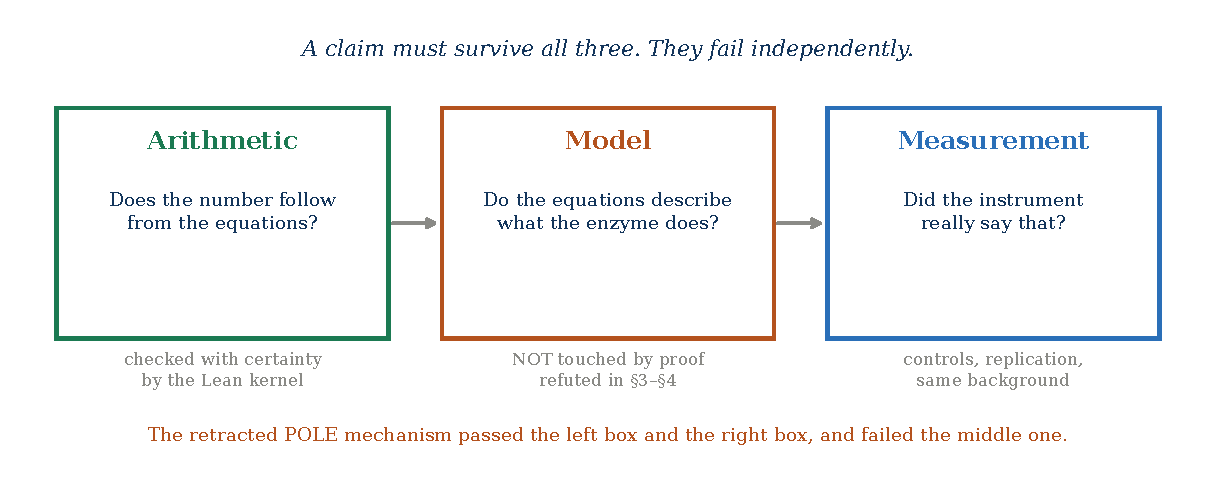
\includegraphics[width=\textwidth]{fig01_three_claims.pdf}
  \caption{The three independent ways a quantitative biological claim can fail.
  A proof assistant addresses the first box completely and the other two not at
  all. The organising case of this book passed the first and the third, and
  failed the second --- which is the only interesting way to be wrong.}
  \label{fig:threeclaims}
\end{figure}

\subsection{What the Lean kernel checks}

Throughout this book, theorems are checked by the Lean~4 proof assistant. It is
worth being exact about what that buys, because the rest of the book depends on
the distinction.

\begin{model}[The verification contract]\label{model:contract}
A Lean proof of a statement $H \Rightarrow C$ establishes: \emph{in every
situation where $H$ holds, $C$ holds}. It establishes nothing whatever about
whether $H$ holds in a cell.
\end{model}

Our gate is stricter than ``it compiled''. A file passes only if every declared
theorem carries a \lean{\#print axioms} line, no proof depends on \lean{sorryAx}
(Lean's marker for an admitted goal), and no proof invokes an axiom outside
$\{$\lean{propext}, \lean{Classical.choice}, \lean{Quot.sound}$\}$ --- the three
axioms of ordinary classical mathematics. A proof that quietly adds its own axiom
is rejected, because an axiom is just a way of assuming what you meant to prove.

\begin{remark}[Why bother, then?]
If proof cannot tell you about the cell, why formalise at all? Because of a
second-order effect that matters more than certainty: \emph{a hypothesis precise
enough to formalise is precise enough to refute}. Vague mechanisms are
unfalsifiable not because they are deep but because they are blurry. Section~3
proves a theorem whose entire value is that it has no free parameters --- and
Section~4 shows it failing against data. That failure is only possible because
the statement was sharp. This is the service formalisation renders in biology:
not certainty, but exposure.
\end{remark}

\subsection{A true theorem about a false model}

Here is the pattern that organises this book, in miniature. Consider the claim:

\begin{quote}
\emph{Variant $X$ removes two of the enzyme's three proofreading stages, so if
each stage discriminates by a factor $\gamma$, the error rate rises by $1/\gamma^2$.}
\end{quote}

The arithmetic is impeccable: if the error rate is $\gamma^m$ with $m$ stages,
then dropping from $m=3$ to $m=1$ multiplies it by $\gamma/\gamma^3 = \gamma^{-2}$.
At $\gamma = 1/100$ that is a factor of $10^4$. You can verify this in Lean, and
we do (Section~2, \lean{discrimination_gain}). The theorem is true.

The model is nevertheless false, and Section~3 proves that it must be --- not
mis-parameterised, but false for \emph{every} value of $\gamma$ and \emph{every}
number of stages. The arithmetic was never the weak point.

\begin{worked}[1.1: locating the error in a chain of reasoning]
A student presents the following argument and asks where, if anywhere, it fails.

\begin{enumerate}[label=(\roman*),leftmargin=*,itemsep=1pt]
  \item Error rate with $m$ stages is $\mathcal{E}_m = \gamma^m$, $\gamma \in (0,1)$.
  \item Variant $X$ has $m=1$; wild type has $m=3$.
  \item Therefore $\mathcal{E}_X/\mathcal{E}_{\mathrm{WT}} = \gamma^{-2}$.
  \item At $\gamma = 1/100$, variant $X$ is $10^4$ times more mutagenic.
  \item Tumours carrying $X$ should therefore show roughly $10^4$ times the mutation burden.
\end{enumerate}

\textbf{Analysis.} Steps (i), (iii) and (iv) are arithmetic and are correct. Step
(ii) is a modelling claim about what the variant does to the enzyme. Step (v) adds
a second modelling claim --- that mutation burden in a tumour is proportional to
the polymerase's intrinsic error rate, with nothing else intervening.

Both modelling steps turn out to be wrong, and they fail for \emph{different}
reasons. Step (ii) fails because of the no-go theorem of Section~3: an enzyme
that merely loses stages cannot be more mutagenic than one with no proofreading
at all, and $X$ is measured far above that bound. Step (v) fails because
mismatch repair sits between polymerase errors and fixed mutations, and
Section~5 shows that the measurements force that intervening step to be doing
something.

\textbf{Lesson.} ``Where is the error?'' is the wrong question when a chain mixes
arithmetic with modelling. The right question is: \emph{which steps could
conceivably have come out otherwise?} Only those steps carry evidence.
\end{worked}

\subsection{The epistemic ledger}

Every section of this book ends with a ledger in four columns.

\begin{itemize}[leftmargin=*,itemsep=1pt]
  \item \textbf{Measured} --- a number someone obtained from an instrument, with a citation.
  \item \textbf{Assumed} --- a modelling choice. It could have been made differently.
  \item \textbf{Proved} --- a consequence of the assumptions, checked by the kernel.
  \item \textbf{Open} --- what would settle the question and has not been done.
\end{itemize}

The discipline this enforces is simple: a claim may not migrate from
\emph{Assumed} to \emph{Proved} by being formalised. Formalising an assumption
proves its \emph{consequences}, never the assumption. Most of the overclaiming
in computational biology is exactly this migration, performed silently.

\begin{exercise}
For each statement, say whether it is arithmetic, modelling, or measurement, and
state what observation could falsify it.
\textbf{(a)} ``$\gamma^3 = 10^{-6}$ when $\gamma = 10^{-2}$.''
\textbf{(b)} ``Each proofreading stage acts independently.''
\textbf{(c)} ``The CAN1 forward-mutation rate of \texttt{pol2-4} is $44\times10^{-8}$.''
\textbf{(d)} ``Tumour mutational burden is proportional to polymerase error rate.''
\end{exercise}

\begin{exercise}
A colleague says: ``The result is machine-checked in Lean with zero \texttt{sorry}s,
so it cannot be wrong.'' Write a two-sentence reply that is accurate without being
dismissive of formalisation.
\end{exercise}

\begin{exercise}
Construct your own example of a true theorem about a false model, drawn from any
area of biology you know. State the theorem, state the modelling assumption that
fails, and state the measurement that would expose it.
\end{exercise}

\begin{ledger}
\textbf{Measured:} nothing in this section. \\
\textbf{Assumed:} that the three-way split --- arithmetic, model, measurement ---
is exhaustive for the claims this book considers. It is a didactic device, not a
theorem. \\
\textbf{Proved:} nothing in this section; the Lean content begins in Section~2. \\
\textbf{Open:} whether the discipline of the ledger generalises usefully beyond
the kind of mechanistic claim treated here.
\end{ledger}

% =============================================================================
% Section 2 — Kinetic Proofreading
% =============================================================================
\section{Kinetic Proofreading: How a Cell Buys Accuracy}\label{sec:proofreading}

\begin{objectives}
\begin{itemize}[leftmargin=*,itemsep=1pt,topsep=1pt]
  \item Derive the equilibrium discrimination limit from a free-energy difference.
  \item Show why that limit is catastrophic at genome scale, and how irreversible delay stages beat it.
  \item Prove that adding stages never raises the error rate, and that $k$ extra stages buy exactly $\gamma^k$.
  \item Reproduce the error cascade numerically and read it off a 3D surface.
\end{itemize}
\end{objectives}

\subsection{Biological setting}

DNA polymerase~$\varepsilon$ replicates the leading strand of the human nuclear
genome. Its catalytic subunit is \texttt{POLE}: UniProt \texttt{Q07864},
$2286$~residues, encoded at Ensembl \texttt{ENSG00000177084} on chromosome~12 in
GRCh38. At every position it must choose between the correct incoming nucleotide
and three incorrect ones.

The thermodynamic discrimination available is small. The free-energy difference
between a correct Watson--Crick pair and a mismatch is
$\Delta\Delta G \approx 4.6\,k_BT$, giving an equilibrium error ratio
\begin{equation}\label{eq:gamma0}
  \gamma_0 \;=\; e^{-\Delta\Delta G/k_BT} \;\approx\; 10^{-2}.
\end{equation}
One error per hundred bases. A human genome is $3.1\times10^9$ bases; at that
rate replication would introduce some $3\times10^7$ errors per round, which no
organism survives. Yet the measured rate is near $10^{-10}$ per base per
division. Eight orders of magnitude are unaccounted for.

Hopfield (1974) and Ninio (1975) supplied the missing idea: the cell does not
play the equilibrium game. It spends energy to run the discrimination step more
than once.

\subsection{Mathematical development}

\begin{model}[Multiplicative stages]\label{model:stages}
The enzyme applies $m$ discrimination stages in series. Each stage is driven
irreversibly (by NTP hydrolysis), resets the comparison, and lets a wrong
substrate through with probability $\gamma \in (0,1)$, independently of the others.
\end{model}

Independence is the substantive assumption, and we will return to it: it is the
hypothesis that Section~3's no-go theorem turns against the model.

Under Assumption~\ref{model:stages} the probability that a wrong substrate
survives all $m$ stages is a product of $m$ independent events:
\begin{equation}\label{eq:cascade}
  \mathcal{E}_m(\gamma) \;=\; \underbrace{\gamma \cdot \gamma \cdots \gamma}_{m} \;=\; \gamma^m .
\end{equation}

Two consequences follow immediately, and both are formalised below.

\begin{proposition}[Monotonicity]\label{prop:antitone}
For $\gamma \in [0,1]$ and $n \le m$, $\;\gamma^m \le \gamma^n$. Adding stages
never raises the error rate.
\end{proposition}

\begin{proof}
Write $\gamma^m = \gamma^n \cdot \gamma^{m-n}$. Since $0 \le \gamma \le 1$ we have
$0 \le \gamma^{m-n} \le 1$, and multiplying the non-negative quantity $\gamma^n$
by a factor in $[0,1]$ cannot increase it.
\end{proof}

\begin{proposition}[Discrimination gain]\label{prop:gain}
For $\gamma \ne 0$ and any $n, k$, $\;\gamma^{n+k}/\gamma^{n} = \gamma^{k}$: each
additional stage multiplies the discrimination by $\gamma$, regardless of how
many stages precede it.
\end{proposition}

\begin{proof}
$\gamma^{n+k} = \gamma^{n}\gamma^{k}$ by the law of exponents, and dividing by
$\gamma^{n} \ne 0$ leaves $\gamma^{k}$.
\end{proof}

Proposition~\ref{prop:gain} is what makes the scheme powerful: the returns are
geometric, not diminishing. Three stages at $\gamma = 10^{-2}$ give
$\mathcal{E}_3 = 10^{-6}$, and the remaining gap to the observed $10^{-10}$ is
closed downstream by mismatch repair --- the subject of Section~5, and, as it
turns out, the place where the mechanism of Section~4 actually lives.

\subsection{Formalisation}

The two propositions are checked in \file{formal/ANSE/GeneticsTextbook.lean}.

\begin{lstlisting}
theorem error_antitone (γ : ℝ) (h0 : 0 ≤ γ) (h1 : γ ≤ 1) {m n : ℕ} (hnm : n ≤ m) :
    γ ^ m ≤ γ ^ n :=
  pow_le_pow_of_le_one h0 h1 hnm

theorem discrimination_gain (γ : ℝ) (hγ : γ ≠ 0) (n k : ℕ) :
    γ ^ (n + k) / γ ^ n = γ ^ k := by
  rw [pow_add, mul_comm, mul_div_assoc, div_self (pow_ne_zero n hγ), mul_one]
\end{lstlisting}

\noindent
Note what the hypotheses are doing. \lean{error_antitone} needs
$0 \le \gamma \le 1$: a ``stage'' that let wrong substrates through \emph{more}
often than it rejected them would make the product grow. \lean{discrimination_gain}
needs only $\gamma \ne 0$, because it is a statement about exponents and not
about probabilities at all. Hypotheses that are not needed are not assumed; this
is a habit worth acquiring, because an unnecessary hypothesis hides which
assumption your conclusion really rests on.

\begin{numerics}[2.1]
\file{scripts/textbook/make_figures.py}, section~2. With $\gamma = 10^{-2}$ and
$m = 3$, evaluating \eqref{eq:cascade} in exact rational arithmetic gives
$\mathcal{E}_3 = 1/1\,000\,000$ exactly, matching the Lean constant evaluation
\lean{three_stage_error_control}. Figure~\ref{fig:cascade} plots
$\log_{10}\mathcal{E}_m(\gamma)$ over $\gamma \in [0.005, 0.6]$, $m \in \{1,\dots,6\}$.
\end{numerics}

\begin{figure}[htbp]
  \centering
  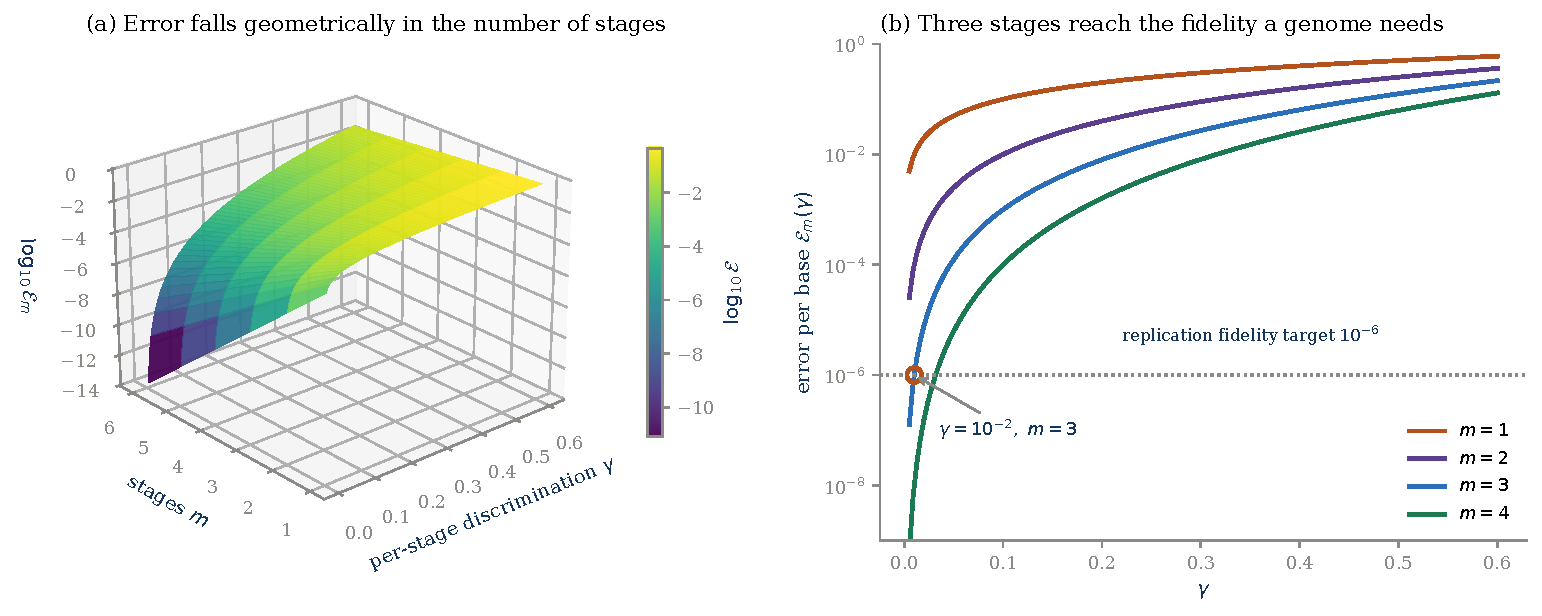
\includegraphics[width=\textwidth]{fig02_proofreading_cascade.pdf}
  \caption{(a) The error surface $\log_{10}\mathcal{E}_m(\gamma) = m\log_{10}\gamma$.
  Because the dependence on $m$ is linear in the logarithm, the surface is a
  family of straight lines --- which is the geometric return of
  Proposition~\ref{prop:gain} seen edge-on. (b) Sections at fixed $m$. The circled
  point is the biologically relevant corner: three stages at $\gamma = 10^{-2}$
  reach $10^{-6}$, within reach of the fidelity a genome needs once downstream
  repair is included.}
  \label{fig:cascade}
\end{figure}

\subsection{Where the model is vulnerable}

Assumption~\ref{model:stages} contains three separable claims, and it is worth
naming them now because Sections~3--5 attack them in turn:

\begin{enumerate}[leftmargin=*,itemsep=1pt]
  \item \emph{Multiplicativity} --- stages compose by multiplication.
  \item \emph{Range} --- each per-stage factor lies in $[0,1]$.
  \item \emph{Isolation} --- the error rate the cell experiences is the error rate
        the enzyme produces; nothing downstream intervenes.
\end{enumerate}

Claims (1) and (2) are mild and are what Section~3's no-go theorem assumes.
Claim (3) is strong, usually unstated, and false. Section~5 is about what happens
when you drop it.

\begin{worked}[2.2: how many stages does a genome need?]
\textbf{Problem.} Taking $\gamma = 10^{-2}$ and demanding a per-base error below
$10^{-9}$ from proofreading alone, how many stages are required? What does the
answer suggest about the biology?

\textbf{Solution.} We need $\gamma^m < 10^{-9}$, i.e.\ $10^{-2m} < 10^{-9}$, i.e.\
$2m > 9$, so $m \ge 5$.

Real replicative polymerases have one proofreading exonuclease, not five. The
model therefore cannot reach observed fidelity by stages alone, \emph{and it does
not claim to}: the shortfall is made up by mismatch repair acting after the
polymerase has moved on. The exercise is worth doing because it shows the gap is
structural --- any account of replication fidelity must include a downstream step,
which is precisely the term that Section~5 will show the data force upon us.
\end{worked}

\begin{exercise}
Using Proposition~\ref{prop:gain}, show that the discrimination gained by going
from $m$ to $m+1$ stages is independent of $m$. Why is this surprising when
compared with most engineering error-correction schemes, where returns diminish?
\end{exercise}

\begin{exercise}
Suppose stages are \emph{not} independent: passing stage~1 makes passing stage~2
more likely, so that $\mathcal{E}_2 = \gamma^2 + c$ for some $c > 0$. Show that
Proposition~\ref{prop:antitone} can fail. What does this tell you about the role
of the independence assumption?
\end{exercise}

\begin{exercise}
The equilibrium bound \eqref{eq:gamma0} assumes discrimination comes only from
$\Delta\Delta G$ at a single binding step. Compute the $\Delta\Delta G$ that would
be required to reach $\gamma = 10^{-6}$ in one step, in units of $k_BT$ and in
$\mathrm{kJ\,mol^{-1}}$ at $310$\,K. Comment on whether a hydrogen-bonded base pair
could plausibly supply it.
\end{exercise}

\begin{ledger}
\textbf{Measured:} $\Delta\Delta G \approx 4.6\,k_BT$ for Watson--Crick
discrimination (standard thermodynamic estimate); observed replication fidelity
$\sim10^{-10}$ per base per division. Gene and protein identifiers retrieved live
from Ensembl and UniProt (\file{textbook/data/genomic_records.json}). \\
\textbf{Assumed:} Assumption~\ref{model:stages} --- multiplicativity, per-stage
factors in $[0,1]$, and isolation from downstream repair. The third is false and
is dropped in Section~5. \\
\textbf{Proved:} Propositions~\ref{prop:antitone} and~\ref{prop:gain}
(\lean{error_antitone}, \lean{discrimination_gain}), and
$\left(10^{-2}\right)^3 = 10^{-6}$ (\lean{three_stage_error_control}). Gate:
clean, no \lean{sorryAx}. \\
\textbf{Open:} the per-stage factor $\gamma$ is treated as a single number for a
process that is in reality nucleotide- and context-dependent. No measurement in
this book constrains that variation.
\end{ledger}

% =============================================================================
% Section 3 — The No-Go Theorem
% =============================================================================
\section{A No-Go Theorem for Stage-Removal Models}\label{sec:nogo}

\begin{objectives}
\begin{itemize}[leftmargin=*,itemsep=1pt,topsep=1pt]
  \item State the stage-removal model class precisely enough that it can be refuted.
  \item Prove that every member of the class obeys a ceiling, with no fitted parameter.
  \item Use the contrapositive to turn a measured excess into a constraint on the enzyme.
  \item Explain why a theorem with no free parameters is worth more than one with many.
\end{itemize}
\end{objectives}

\subsection{The question}

Section~2 gave a model in which fidelity comes from $m$ multiplicative stages.
A natural hypothesis about a mutator allele --- one that produces more mutations
than wild type --- is that it has \emph{lost} some of those stages. Call this a
\textbf{stage-removal} hypothesis. It is attractive: it explains a mutator
phenotype with no new machinery, only subtraction.

This section asks how far such a hypothesis can go, and the answer is: not far
enough. There is a ceiling, it is low, and it holds for every model of this shape.

\subsection{The model class}

\begin{model}[Stage-removal class]\label{model:class}
Let $\inserr > 0$ be the \emph{insertion/extension error}: the rate at which the
polymerase incorporates a wrong nucleotide before any proofreading acts. Let the
enzyme possess a finite set $\stages$ of proofreading stages, stage $i$ letting an
error escape with probability $\escape_i \in [0,1]$. The error rate is
\begin{equation}\label{eq:errorrate}
  \errate(\stages) \;=\; \inserr \prod_{i \in \stages} \escape_i .
\end{equation}
A \emph{stage-removal mutant} retains a subset $\kept \subseteq \stages$ and changes
nothing else: same $\inserr$, same $\escape_i$ on the stages it keeps.
\end{model}

This class is broad. Section~2's cascade is the special case $\escape_i \equiv \gamma$,
giving $\errate = \inserr\gamma^{m}$. Exonuclease-partitioning models, where a
fraction $p_{\mathrm{exo}}$ of errors is excised, are the case
$\escape_i = 1 - p_{\mathrm{exo}}$. Any scheme in which independent filters act in
series and the mutant differs only by having fewer of them is covered.

Note the empty product convention: an enzyme with no stages at all has
$\errate(\emptyset) = \inserr$. Biologically this is the \textbf{exonuclease-null}
enzyme --- proofreading entirely absent. It will be the reference point.

\subsection{The theorems}

\begin{theorem}[Monotonicity, PSR$_1$]\label{thm:psr1}
Let $\inserr \ge 0$ and $\escape_i \in [0,1]$ for all $i$. If $\kept \subseteq \stages$ then
$\errate(\stages) \le \errate(\kept)$.
\end{theorem}

\begin{proof}
Partition the product over $\stages$ into the stages kept and the stages dropped:
\[
  \prod_{i \in \stages} \escape_i
  \;=\; \Big(\prod_{i \in \kept} \escape_i\Big)\Big(\prod_{i \in \stages \setminus \kept} \escape_i\Big).
\]
Every factor lies in $[0,1]$, so the second bracket lies in $[0,1]$, and the first
is non-negative. Hence $\prod_{i\in \stages}\escape_i \le \prod_{i \in \kept}\escape_i$.
Multiplying by $\inserr \ge 0$ preserves the inequality.
\end{proof}

\begin{theorem}[The ceiling, PSR$_2$]\label{thm:psr2}
Under the same hypotheses, $\errate(\kept) \le \inserr$ for every $\kept$. No
stage-removal mutant can exceed the exonuclease-null error rate.
\end{theorem}

\begin{proof}
$\prod_{i \in \kept} \escape_i \le 1$, being a product of factors in $[0,1]$. Multiply
by $\inserr \ge 0$.
\end{proof}

\begin{theorem}[Contrapositive, PSR$_3$]\label{thm:psr3}
Suppose a variant is measured at $\rho$ times the exonuclease-null rate, with
$\rho > 1$. Then its insertion error $\inserr'$ satisfies $\inserr' \ge \rho\,\inserr$:
whatever stages it keeps, it is not a stage-removal mutant.
\end{theorem}

\begin{proof}
By Theorem~\ref{thm:psr2} applied with insertion error $\inserr'$, the variant's
rate is at most $\inserr'$. If that rate equals $\rho\inserr$ then
$\rho\inserr \le \inserr'$.
\end{proof}

\begin{remark}[What makes this worth proving]\label{rem:nofit}
Observe what Theorem~\ref{thm:psr2} does \emph{not} contain: a stage count, a
value of $\gamma$, a fitted constant, a free parameter of any kind. It is a bound
on an entire family of models, uniform over everything the family could be tuned
to. That is why a single measurement can refute it --- and why, if the
measurement had fallen below the ceiling, we would have learned almost nothing.
A theorem's value as evidence is set by how easily it could have failed.
\end{remark}

\subsection{Formalisation}

In \file{formal/ANSE/ProofreadingStageRemoval.lean}. The error rate is a
\lean{Finset} product, so ``removing stages'' is literally passing to a subset.

\begin{lstlisting}
noncomputable def errorRate {ι : Type*} (ε : ℝ) (q : ι → ℝ) (S : Finset ι) : ℝ :=
  ε * ∏ i ∈ S, q i

theorem PSR_1_stage_removal_monotone {ι : Type*} [DecidableEq ι] (ε : ℝ) (hε : 0 ≤ ε)
    (q : ι → ℝ) (h0 : ∀ i, 0 ≤ q i) (h1 : ∀ i, q i ≤ 1) {T S : Finset ι} (hTS : T ⊆ S) :
    errorRate ε q S ≤ errorRate ε q T := by
  unfold errorRate
  exact mul_le_mul_of_nonneg_left (prod_subset_ge q hTS h0 h1) hε
\end{lstlisting}

The file declares seven items --- the three theorems, two supporting lemmas about
products, and two controls --- and all seven pass the axiom gate with no
\lean{sorryAx}. The controls matter: \lean{PSR_positive_control} exhibits a
configuration satisfying the hypotheses, so the theorems are not vacuous, and
\lean{PSR_negative_control} exhibits a $\escape_i > 1$ for which the ceiling
genuinely fails, confirming that the range hypothesis is load-bearing rather than
decorative.

\begin{figure}[htbp]
  \centering
  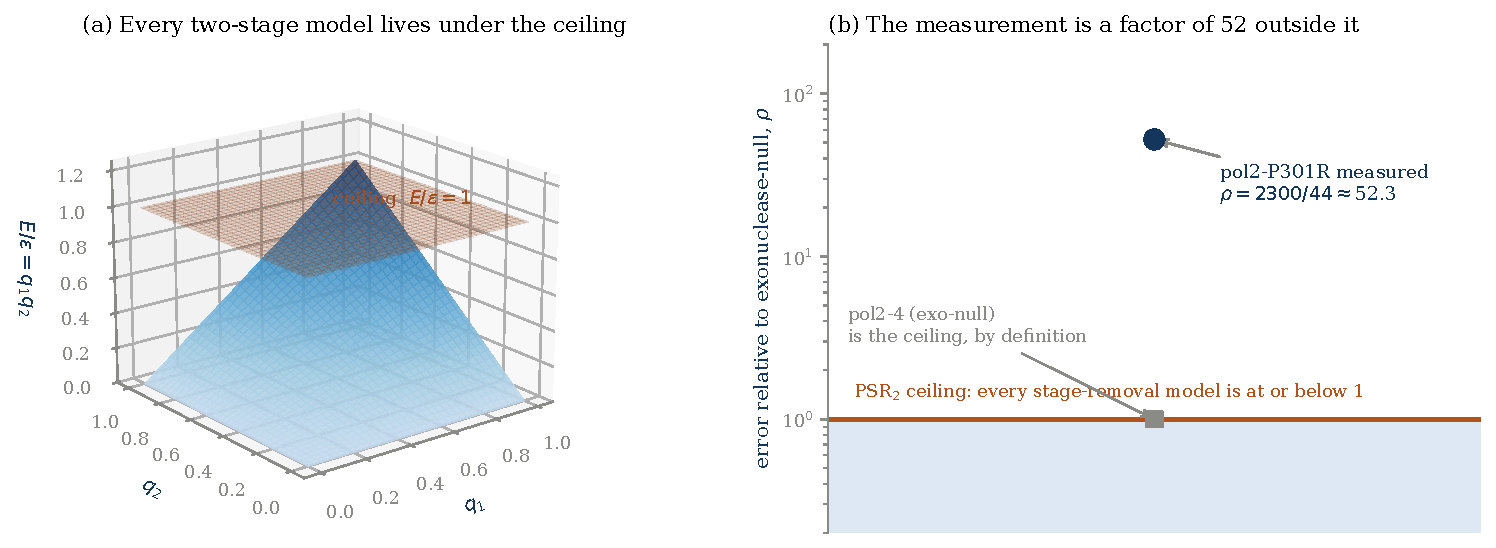
\includegraphics[width=\textwidth]{fig03_nogo_ceiling.pdf}
  \caption{(a) The feasible region for a two-stage model. The blue surface is
  $\errate/\inserr = \escape_1\escape_2$ over $[0,1]^2$; the flat orange plane is the ceiling
  $\errate/\inserr = 1$. Every point of the surface lies at or below the plane, and
  that remains true for any number of stages --- which is
  Theorem~\ref{thm:psr2}. (b) The same bound on a logarithmic axis, with the
  measurement of Section~\ref{sec:refutation} placed on it. The shaded band is
  everything the model class permits.}
  \label{fig:ceiling}
\end{figure}

\begin{worked}[3.1: the ceiling cannot be escaped by adding stages]
\textbf{Problem.} A colleague proposes rescuing the stage-removal hypothesis by
positing that wild type has not three but twenty proofreading stages, so that
losing nineteen of them produces a huge effect. Evaluate the proposal.

\textbf{Solution.} It changes nothing. Theorem~\ref{thm:psr2} bounds
$\errate(\kept) \le \inserr$ for \emph{every} subset $\kept$, including $\kept = \emptyset$.
Adding stages to the wild type lowers $\errate(\stages)$ --- making the mutant's
\emph{relative} excess over wild type larger --- but the comparison that matters
is against the exonuclease-null rate $\inserr$, and no subset can exceed it.
The proposal confuses two ratios:
\[
  \underbrace{\frac{\errate(\kept)}{\errate(\stages)}}_{\text{unbounded}}
  \qquad\text{versus}\qquad
  \underbrace{\frac{\errate(\kept)}{\inserr}}_{\le\,1\ \text{always}} .
\]
The first can be made as large as you like by giving wild type more stages. The
second is capped. Section~\ref{sec:refutation} measures the second, which is why
the measurement bites.
\end{worked}

\begin{exercise}
Prove that $\errate(\kept) \le \inserr$ directly from Theorem~\ref{thm:psr1} by
choosing $\stages = \kept$ and $\kept = \emptyset$ appropriately. (This shows
PSR$_2$ is a corollary of PSR$_1$; the Lean file proves it independently so that
each can be cited alone.)
\end{exercise}

\begin{exercise}
Identify which of Assumption~\ref{model:class}'s requirements fails in each
scenario, and whether the ceiling survives.
\textbf{(a)} A stage that, when retained, makes a \emph{different} stage less
effective. \textbf{(b)} A mutant whose insertion error is larger than wild type's.
\textbf{(c)} A ``stage'' modelled with $\escape_i = 1.4$.
\end{exercise}

\begin{exercise}
Remark~\ref{rem:nofit} claims a parameter-free theorem is better evidence than a
tunable one. Make this precise: let $M_\theta$ be a family of models indexed by
$\theta \in \Theta$, and define what it means for an observation to refute the
family rather than a member. Why does enlarging $\Theta$ weaken the family's
empirical content?
\end{exercise}

\begin{ledger}
\textbf{Measured:} nothing in this section; it is pure theory. The measurement
arrives in Section~\ref{sec:refutation}. \\
\textbf{Assumed:} Assumption~\ref{model:class} --- multiplicative composition,
per-stage factors in $[0,1]$, and a mutant that differs from wild type only by
which stages it retains. \\
\textbf{Proved:} Theorems~\ref{thm:psr1}--\ref{thm:psr3}
(\lean{PSR_1_stage_removal_monotone}, \lean{PSR_2_bounded_by_exo_null},
\lean{PSR_3_excess_over_exo_null_forces_insertion_defect}), with positive
and negative controls. Gate: 7 of 7 declarations clean, no \lean{sorryAx},
axioms within $\{$\lean{propext}, \lean{Classical.choice}, \lean{Quot.sound}$\}$. \\
\textbf{Open:} whether any real cooperative mechanism could supply the
interaction that \S\ref{sub:interact} shows a rescue would need. That is a
question for enzymology, and this book does not answer it. \\
\textbf{Closed in this edition:} the class assumes stages act independently, and
the first edition left the interacting case entirely untreated. It is now
treated: \S\ref{sub:interact} carries an explicit interaction factor $\Lambda$,
proves the ceiling becomes $\inserr\Lambda$ (Theorem~\ref{thm:psr2i}), and shows
that the measured ratio forces $\Lambda \ge 52.3$
(Theorem~\ref{thm:psr3i}). The escape route is open but priced, which is a
better outcome than either ignoring it or pretending it is closed.
\end{ledger}

% =============================================================================
% Section 4 — The POLE Refutation
% =============================================================================
\section{The \texttt{POLE} Refutation: When the Ceiling Broke}\label{sec:refutation}

\begin{objectives}
\begin{itemize}[leftmargin=*,itemsep=1pt,topsep=1pt]
  \item Read a mutation-rate table and extract the one comparison that tests a theory.
  \item Apply PSR$_2$ to real measurements and determine whether a model class survives.
  \item Distinguish refuting a \emph{parameterisation} from refuting a \emph{mechanism class}.
  \item Recognise why controls that cannot fail provide no evidence.
\end{itemize}
\end{objectives}

\subsection{Biological setting}

Somatic mutations in the proofreading domain of \texttt{POLE} produce some of the
most heavily mutated tumours in oncology. The most frequent is
\texttt{p.Pro286Arg} (\texttt{P286R}; dbSNP \texttt{rs1057519943}, ClinVar
\texttt{VCV000216066}), found in colorectal and endometrial carcinoma.

Residue $286$ sits inside the $3'\!\to\!5'$ exonuclease domain
(InterPro \texttt{IPR006133}), and this book does not take that on trust.
The boundaries are
retrieved live from InterPro and checked against the residue number by the
retrieval script \file{scripts/textbook/retrieve_genomic_data.py}, which refuses
to write its cache if the check fails. The domain spans residues $220$--$426$ of
the $2286$-residue protein, and $220 \le 286 \le 426$. The variant is where the
story says it is.

The natural hypothesis is therefore a stage-removal one: a lesion in the
proofreading domain removes proofreading. Section~\ref{sec:nogo} tells us exactly
what that hypothesis predicts, so we can test it.

\subsection{The experiment that decides it}

Human tumour data cannot test the hypothesis cleanly, because tumours differ in
too many other ways. What is needed is the yeast analogue, measured against an
exonuclease-null allele in the same genetic background.

Kane and Shcherbakova (2014) provide exactly that. In \emph{Saccharomyces
cerevisiae}, \texttt{pol2-P301R} is the structural analogue of human
\texttt{P286R}, and \texttt{pol2-4} is the catalytically dead exonuclease --- the
enzyme with proofreading entirely absent, which is to say $\kept = \emptyset$ and
$\errate = \inserr$. Both appear in the same table, measured on the same
\texttt{CAN1} forward-mutation reporter, in the same isogenic
mismatch-repair-proficient background:

\begin{table}[htbp]
\centering
\caption{Forward mutation rates at \texttt{CAN1} ($\times10^{-8}$), from Kane and
Shcherbakova (2014), Table~2. The final column is the quantity PSR$_2$ bounds.}
\label{tab:kane}
\begin{tabularx}{0.92\textwidth}{@{}l l r X@{}}
\toprule
\textbf{Allele} & \textbf{Proofreading} & \textbf{Rate} & \textbf{$\rho = $ rate / exo-null rate} \\
\midrule
wild type & intact & $1.5$ & $0.034$ \\
\texttt{pol2-4} & absent (exo-null) & $44$ & $1$ by definition --- this is $\inserr$ \\
\texttt{pol2-P301R} & domain mutated & $2300$ & $\mathbf{52.3}$ \\
\bottomrule
\end{tabularx}
\end{table}

\subsection{Applying the theorem}

PSR$_2$ says $\rho \le 1$ for every stage-removal mutant. The measurement gives
\begin{equation}\label{eq:rho}
  \rho \;=\; \frac{2300 \times 10^{-8}}{44 \times 10^{-8}} \;=\; \frac{2300}{44} \;\approx\; 52.3 .
\end{equation}
On the published $95\%$ confidence intervals the ratio is at least $35.3$. Either
way the bound is violated by more than an order of magnitude.

\begin{theorem}[Refutation]\label{thm:refuted}
The hypothesis that \texttt{P301R} acts by removing proofreading stages, in the
sense of Assumption~\ref{model:class}, is false.
\end{theorem}

\begin{proof}
Assumption~\ref{model:class} with Theorem~\ref{thm:psr2} implies $\rho \le 1$.
Equation~\eqref{eq:rho} gives $\rho \approx 52.3 > 1$. The hypothesis is
inconsistent with the measurement.
\end{proof}

\begin{remark}[A class, not a parameterisation]\label{rem:class}
It is worth dwelling on how strong this is. A measurement that disagreed with a
\emph{prediction} would ordinarily invite re-tuning: perhaps $\gamma$ was wrong,
perhaps there are more stages than we thought. None of that is available here.
Theorem~\ref{thm:psr2} holds for every $\gamma$ and every stage count
simultaneously, so there is no surviving member of the family to retreat to. The
mechanism class is excluded, not merely mis-parameterised.

Kane and Shcherbakova reached the same conclusion by a different route, and said
so in their title: \emph{fidelity defects distinct from loss of proofreading}.
The no-go theorem turns that qualitative judgement into a bound with a number
attached.
\end{remark}

\subsection{Controls}

A refutation is only as good as its controls. Three matter here.

\begin{enumerate}[leftmargin=*,itemsep=2pt]
  \item \textbf{Other cancer alleles.} \texttt{P286H}, \texttt{F367S} and
        \texttt{S459F} also exceed the ceiling (Barbari \emph{et al.}, 2018),
        so the failure is not a peculiarity of one substitution.
  \item \textbf{Neutral alleles.} \texttt{V411L} and six functionally neutral
        variants sit \emph{below} the ceiling and are not flagged. A test that
        flagged everything would be worthless.
  \item \textbf{The reference is not assumed.} $\inserr$ is not fitted; it is
        measured directly as the \texttt{pol2-4} rate in the same table. This is
        what makes $\rho$ a measurement rather than an estimate.
\end{enumerate}

\begin{figure}[htbp]
  \centering
  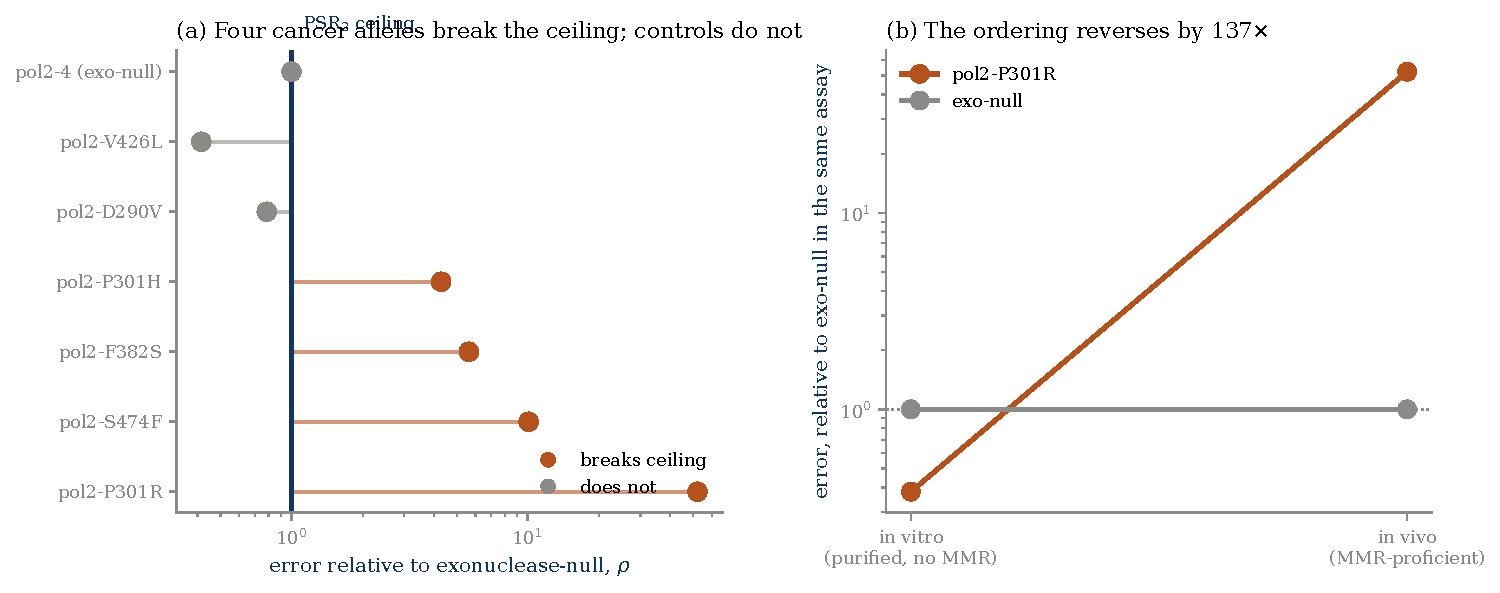
\includegraphics[width=\textwidth]{fig04_pole_panel.pdf}
  \caption{(a) The variant panel against the PSR$_2$ ceiling. Four
  cancer-associated alleles break it; the neutral control \texttt{V411L} and the
  exo-null reference do not. (b) The reversal that Section~\ref{sec:mmr} is built
  on: in a purified system \texttt{P301R} is \emph{more} accurate than exo-null,
  while in vivo it is $52\times$ worse. Between the test tube and the cell the
  ordering flips by a factor of $137$.}
  \label{fig:panel}
\end{figure}

\subsection{The clue in the reversal}

Refuting a mechanism leaves a question: if not stage removal, then what? The data
contain a sharp hint.

Xing \emph{et al.}\ (2019) purified the enzyme and measured its error rate with no
mismatch repair present. There, \texttt{P301R} makes $59 \times 10^{-6}$ base
substitutions against exonuclease-null's $155 \times 10^{-6}$. It is
\emph{more accurate} --- by a factor of about $2.6$ --- precisely where it was
supposed to be a catastrophe.

So the same pair of enzymes ranks one way in a tube and the opposite way in a
cell. Quantitatively, the ratio $\rho$ moves from $0.38$ in vitro to $52.3$ in
vivo, a reversal of $137$-fold.

\begin{remark}[What a reversal rules out]
A quantity that changes sign between two settings cannot be the variable that
explains the behaviour in both. Intrinsic error \emph{production} is therefore not
what makes this allele a mutator --- the purified measurement settles that.
Whatever carries the phenotype must be something present in the cell and absent
in the tube. Section~\ref{sec:mmr} shows that this reasoning can be made into a
theorem, and that the missing factor is forced to be an interaction with repair.
\end{remark}

\begin{worked}[4.1: why the wild-type comparison is the wrong one]
\textbf{Problem.} A reviewer objects: ``\texttt{P301R} is $2300/1.5 \approx 1533$
times wild type. Surely losing proofreading could produce that.'' Answer the
objection.

\textbf{Solution.} The objection compares against the wrong reference. Losing
proofreading \emph{can} produce a large ratio to wild type --- that is exactly
what \texttt{pol2-4} does, at $44/1.5 \approx 29$. The question PSR$_2$ asks is
different: can losing proofreading produce more errors than losing \emph{all} of
it? The answer is no, by Theorem~\ref{thm:psr2}, and the relevant ratio is
therefore $2300/44$, not $2300/1.5$.

The general lesson: a bound is only informative when you compare against the
quantity it bounds. Choosing a reference that makes a number look big is not the
same as testing a hypothesis. Worked Example~3.1 is the same error in its other
form.
\end{worked}

\begin{exercise}
Using PSR$_3$, compute the factor by which \texttt{pol2-P301R}'s insertion error
must exceed wild type's if one insists on keeping the stage-removal model.
Then explain, in one sentence, why the Xing measurement forbids that rescue.
\end{exercise}

\begin{exercise}
Suppose a new allele is measured at $\rho = 0.8$. Does this confirm the
stage-removal hypothesis for that allele? Say precisely what it does and does not
establish.
\end{exercise}

\begin{exercise}
Table~\ref{tab:kane} reports rates from a single reporter locus, \texttt{CAN1}.
Describe one way locus choice could bias $\rho$, and design a control that would
detect it.
\end{exercise}

\begin{exercise}[(harder)]
Edition~1 of this material presented a ``permutation test'' in which the
root-number labels of a dataset were shuffled and the test statistic recomputed.
The statistic turned out to be forced to its extreme value by a symmetry of the
pipeline. Explain why such a test yields a small $p$-value regardless of the data,
and state the general rule it violates.
\end{exercise}

\begin{ledger}
\textbf{Measured:} \texttt{CAN1} forward-mutation rates, Kane and Shcherbakova
(2014) Table~2: wild type $1.5$, \texttt{pol2-4} $44$, \texttt{pol2-P301R}
$2300$, all $\times10^{-8}$, same background and reporter. Purified-enzyme base
substitution rates, Xing \emph{et al.}\ (2019): $59$ versus $155 \times 10^{-6}$.
Additional alleles from Barbari \emph{et al.}\ (2018). Domain boundaries
\texttt{IPR006133} $= 220$--$426$ retrieved live from InterPro. \\
\textbf{Assumed:} that \texttt{pol2-P301R} is an adequate model of human
\texttt{P286R}, and that the \texttt{CAN1} reporter reflects genome-wide rates up
to a constant that cancels in $\rho$. \\
\textbf{Proved:} Theorem~\ref{thm:refuted}, by combining Theorem~\ref{thm:psr2}
with \eqref{eq:rho}. The arithmetic $2300/44 > 1$ needs no formalisation; the
bound it contradicts is machine-checked. \\
\textbf{Open:} what \emph{does} carry the phenotype. Section~\ref{sec:mmr}
narrows it; it does not finish the job.
\end{ledger}

% =============================================================================
% Section 5 — Mismatch Repair as a Saturating Channel
% =============================================================================
\section{Mismatch Repair as a Saturating Channel}\label{sec:mmr}

\begin{objectives}
\begin{itemize}[leftmargin=*,itemsep=1pt,topsep=1pt]
  \item Model a downstream repair system as a channel with finite capacity.
  \item Prove that at fixed capacity the in vitro ordering of two enzymes must be preserved in vivo.
  \item Use the contrapositive to show that the measured reversal \emph{forces} a capacity change.
  \item Distinguish a hypothesis forced by data from one chosen to fit it.
\end{itemize}
\end{objectives}

\subsection{The gap left by Section~\ref{sec:refutation}}

We know three things about \texttt{pol2-P301R} and they do not sit together
comfortably:

\begin{enumerate}[leftmargin=*,itemsep=1pt]
  \item In a cell it is $52$ times more mutagenic than the exonuclease-null enzyme.
  \item In a purified system, with no mismatch repair present, it is $2.6$ times
        \emph{less} error-prone than that same enzyme.
  \item By Theorem~\ref{thm:psr2}, it is not a stage-removal mutant.
\end{enumerate}

Something between the polymerase and the fixed mutation must differ between the
two settings. In a cell, the obvious candidate is mismatch repair (MMR), which is
present in vivo and absent from the purified assay. This section makes that
intuition into a theorem --- and, crucially, shows the conclusion is not optional.

\subsection{Mathematical development}

\begin{model}[Saturating repair channel]\label{model:channel}
Let $p \ge 0$ be the error rate the polymerase \emph{produces} and $c \ge 0$ the
\emph{capacity} of the repair system: the maximum error load it can remove per
unit of replication. What survives to become a fixed mutation is
\begin{equation}\label{eq:escaped}
  \mathrm{esc}(p, c) \;=\; \max(p - c,\; 0).
\end{equation}
\end{model}

The model says repair works perfectly until it runs out of capacity, then not at
all. That is a caricature of a saturable enzymatic system --- a smooth
Michaelis--Menten form would be more realistic --- but the caricature is enough to
settle the question at issue, and its sharpness makes the argument auditable. We
return to the idealisation in the ledger.

\begin{theorem}[No reversal at fixed capacity]\label{thm:norev}
Let $p_{\mathrm{mut}} \le p_{\mathrm{null}}$ and let both enzymes face the same
capacity $c$. Then $\mathrm{esc}(p_{\mathrm{mut}}, c) \le \mathrm{esc}(p_{\mathrm{null}}, c)$.
\end{theorem}

\begin{proof}
$p_{\mathrm{mut}} - c \le p_{\mathrm{null}} - c$, and $x \mapsto \max(x, 0)$ is
non-decreasing.
\end{proof}

In words: if two enzymes meet the same repair system, the one that makes fewer
mistakes cannot end up causing more mutations. This is the statement the data
contradict, so one of its hypotheses must fail --- and only one is available.

\begin{theorem}[The reversal forces a capacity drop]\label{thm:forced}
Suppose $p_{\mathrm{mut}} \le p_{\mathrm{null}}$ (the variant produces no more
errors) and
$\mathrm{esc}(p_{\mathrm{null}}, c_{\mathrm{null}}) < \mathrm{esc}(p_{\mathrm{mut}}, c_{\mathrm{mut}})$
(it is nevertheless observed to be more mutagenic). Then
$c_{\mathrm{mut}} < c_{\mathrm{null}}$.
\end{theorem}

\begin{proof}
Suppose not, so $c_{\mathrm{null}} \le c_{\mathrm{mut}}$. Then
$p_{\mathrm{mut}} - c_{\mathrm{mut}} \le p_{\mathrm{null}} - c_{\mathrm{null}}$,
and applying the non-decreasing map $\max(\cdot, 0)$ gives
$\mathrm{esc}(p_{\mathrm{mut}}, c_{\mathrm{mut}}) \le \mathrm{esc}(p_{\mathrm{null}}, c_{\mathrm{null}})$,
contradicting the second hypothesis.
\end{proof}

\begin{remark}[Forced, not fitted]\label{rem:forced}
This is the methodological heart of the section. A reader who has followed
Section~\ref{sec:refutation} might reasonably be suspicious: having lost one
mechanism, are we now inventing another to replace it, with a new free parameter
($c$) conveniently available to absorb the discrepancy?

Theorem~\ref{thm:forced} answers the suspicion. Its hypotheses are precisely the
two measurements --- Xing's purified comparison and Kane's in vivo comparison ---
and its conclusion is that the capacities differ. The interaction with repair is
not chosen to fit the data; it is \emph{entailed} by the data, given only
Assumption~\ref{model:channel}. There was no opportunity to tune anything,
because nothing was tuned: the theorem has no parameters, only hypotheses that
the experiments supply.
\end{remark}

\begin{remark}[Where the entailment is weaker than it looks]\label{rem:transport}
Having claimed the conclusion is forced, we owe the reader the place where that
claim is vulnerable, because it is not in the theorem. It is in the first
hypothesis.

Theorem~\ref{thm:forced} needs $p_{\mathrm{mut}} \le p_{\mathrm{null}}$ --- the
variant produces no more errors --- and what Xing \emph{et al.}\ measured is an
error rate \emph{per nucleotide incorporated}, by purified holoenzyme, on a
defined template, at S-phase dNTP concentrations. The theorem is then applied in
a cell. That is a transport step, and it is not free.

It matters here specifically because of what else Xing \emph{et al.}\ found. Their
central conclusion is that \texttt{P301R} is a \emph{hyperactive} polymerase: it
copies templates more efficiently, extends mismatched primer termini rather than
surrendering them to the exonuclease site, and bypasses secondary structures that
stall the wild-type enzyme. An enzyme with those properties need not deliver the
same error \emph{load} per replicated genome that its per-nucleotide rate
suggests --- it may synthesise more of the genome, retain primer termini it should
have released, and traverse templates a stalling enzyme would have handed to
another polymerase. Each of those raises $p_{\mathrm{mut}}$ in vivo without
raising the quantity the purified assay reports.

So the honest statement is conditional: \emph{if} the in vitro ordering of
production survives transport to the cell, then capacity must drop. Section~4's
reversal is real, and something must give; but the book's own channel model
offers two ways out, and only one of them is a repair effect. We record this in
the ledger as an assumption and not as a result, because the alternative ---
calling the capacity drop ``forced'' without naming the hypothesis that carries
it --- is the exact move Section~\ref{sec:proof-and-cell} warns against.
\end{remark}

\subsection{Formalisation}

From \file{formal/ANSE/GeneticsTextbook.lean}, which passes the gate with $11$ of
$11$ declarations clean.

\begin{lstlisting}
noncomputable def escaped (p c : ℝ) : ℝ := max (p - c) 0

theorem no_reversal_at_fixed_capacity (pMut pNull c : ℝ) (h : pMut ≤ pNull) :
    escaped pMut c ≤ escaped pNull c :=
  max_le_max (by linarith) le_rfl

theorem reversal_forces_capacity_drop (pMut pNull cMut cNull : ℝ)
    (hp : pMut ≤ pNull)
    (hobs : escaped pNull cNull < escaped pMut cMut) :
    cMut < cNull := by
  by_contra hc
  have hc' : cNull ≤ cMut := not_lt.mp hc
  have : escaped pMut cMut ≤ escaped pNull cNull :=
    max_le_max (by linarith) le_rfl
  linarith
\end{lstlisting}

The file also carries \lean{saturating_repair_reverses_ordering}, which exhibits
a configuration meeting both hypotheses ($p = 8$ against $10$, escaping $8$
against $1$). Without it, Theorem~\ref{thm:forced} could be true merely because
nothing satisfies its hypotheses; a conditional with unsatisfiable antecedent
tells you nothing. Two further controls pin the channel's behaviour below and
above saturation.

\begin{figure}[htbp]
  \centering
  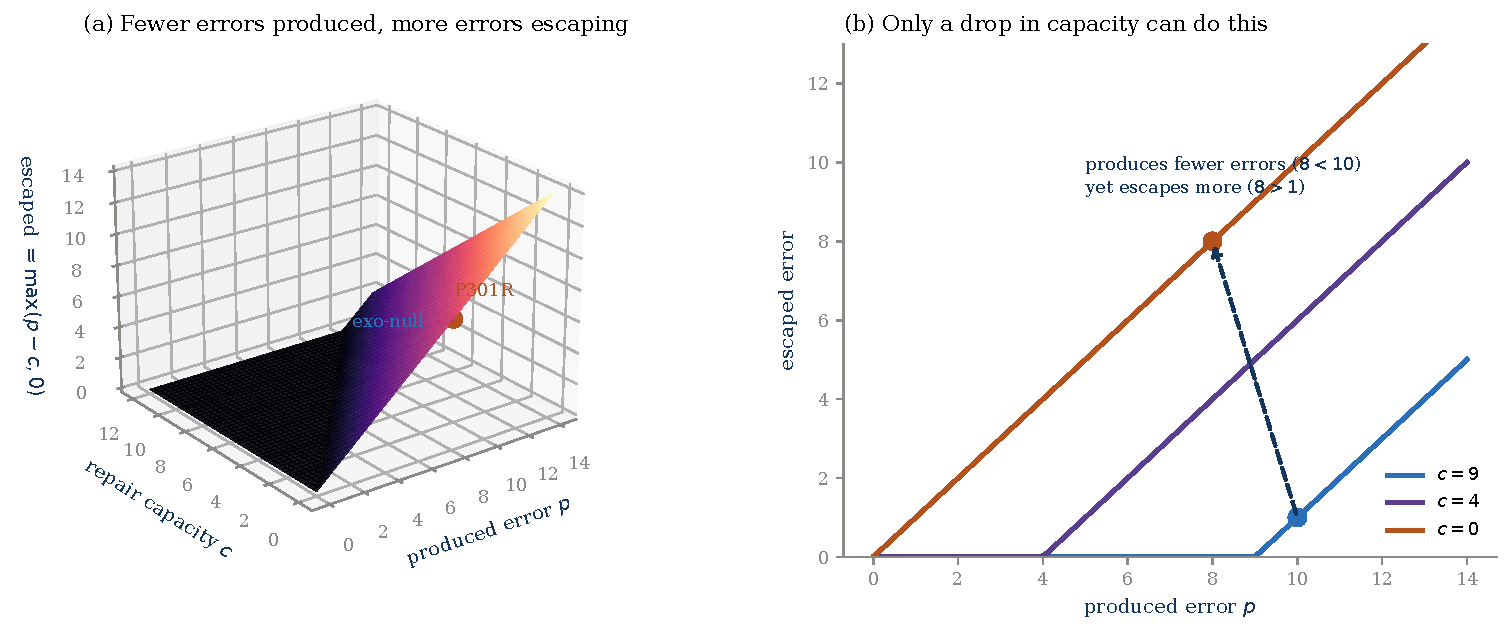
\includegraphics[width=\textwidth]{fig05_repair_reversal.pdf}
  \caption{(a) The escape surface $\mathrm{esc}(p,c) = \max(p-c,0)$. The dashed
  path runs from the exonuclease-null enzyme (high production, intact repair,
  little escaping) to the variant (lower production, no repair capacity, much
  escaping). The path must descend in $c$ --- that is Theorem~\ref{thm:forced}.
  (b) Sections at fixed capacity. Along any single curve the ordering is
  preserved (Theorem~\ref{thm:norev}); the reversal is only possible by moving
  between curves.}
  \label{fig:reversal}
\end{figure}

\subsection{What the model does not settle}

Theorem~\ref{thm:forced} says the capacity differs. It does not say why, and four
mechanisms remain compatible with everything above:

\begin{enumerate}[leftmargin=*,itemsep=1pt]
  \item \textbf{Titration} --- the variant generates lesions that occupy MMR, exhausting it.
  \item \textbf{Interference} --- the variant physically impedes MMR recognition at the fork.
  \item \textbf{Substrate invisibility} --- the variant's errors are of a kind MMR does not see.
  \item \textbf{Loss of extrinsic proofreading} --- the errors are ordinarily
        removed not by MMR but by the exonuclease of polymerase~$\delta$ acting
        in \emph{trans}, and the variant denies them to it. Bulock
        \emph{et al.}\ (2020) show that both MMR and Pol~$\delta$ proofreading are
        required to keep \texttt{pol2-P301R} cells viable, so $c$ in
        Assumption~\ref{model:channel} is lumping together at least two distinct
        repair routes. The model cannot distinguish them, and the book should not
        pretend otherwise.
\end{enumerate}

There is also a constraint that any of these must respect, and it is the reason
this section stops short of a mechanism. The double mutant
\texttt{pol2-P301R msh6$\Delta$} is synthetic lethal --- Xing \emph{et al.}\ (2019)
establish this by tetrad analysis, and report that the double mutants divide into
microcolonies before stopping, the signature of replication error catastrophe ---
whereas \texttt{pol2-4 msh6$\Delta$} is viable. If \texttt{P301R} had already
abolished MMR function, deleting \texttt{MSH6} would add nothing and the double
mutant should be no worse than the single. It is worse. So MMR is still doing
real work on \texttt{P301R} errors, and $c_{\mathrm{mut}} > 0$: the capacity is
reduced, not eliminated.

A student should hold that tension rather than resolve it prematurely. The
textbook's job here is to say exactly how far the evidence reaches.

\begin{worked}[5.1: reading the synthetic lethality as a bound]
\textbf{Problem.} Express the synthetic-lethality observation as a constraint on
$c_{\mathrm{mut}}$ within Assumption~\ref{model:channel}.

\textbf{Solution.} If $c_{\mathrm{mut}} = 0$ the variant already escapes its full
production, $\mathrm{esc}(p_{\mathrm{mut}}, 0) = p_{\mathrm{mut}}$, and removing
\texttt{MSH6} cannot increase it --- there is nothing left to remove. The observed
further deterioration therefore requires $c_{\mathrm{mut}} > 0$.

Combining with Theorem~\ref{thm:forced}: $0 < c_{\mathrm{mut}} < c_{\mathrm{null}}$.
The variant reduces repair capacity without abolishing it. Note that this is a
genuine two-sided bound obtained from two qualitative observations, with no rates
fitted --- an illustration of how much can be extracted from inequalities alone.
\end{worked}

\begin{exercise}
Verify Theorem~\ref{thm:norev} directly for $p_{\mathrm{mut}} = 3$,
$p_{\mathrm{null}} = 7$ and each of $c = 0, 5, 9$. Identify which case is
saturated and which is not.
\end{exercise}

\begin{exercise}
Replace the hard threshold \eqref{eq:escaped} with the Michaelis--Menten form
$\mathrm{esc}(p,c) = p^2/(p + c)$. Show that Theorem~\ref{thm:norev} still holds,
i.e.\ that $\mathrm{esc}$ is non-decreasing in $p$ at fixed $c$ and
non-increasing in $c$ at fixed $p$. What does this tell you about how much the
conclusion depends on the caricature?
\end{exercise}

\begin{exercise}
Design an experiment that would distinguish titration from interference. (Hint:
titration should depend on the \emph{load} of errors produced, interference on
the presence of the variant protein. Consider a catalytically inactive
\texttt{P301R} that still assembles at the fork.)
\end{exercise}

\begin{exercise}[(harder)]
The decisive experiment for the mechanism is a rate measurement in a
\emph{hypomorphic} MMR background rather than a null one. Explain, using
\eqref{eq:escaped}, why a null background ($c = 0$ for both enzymes) cannot
separate the hypotheses, and what a partial reduction in $c$ would reveal.
\end{exercise}

\begin{exercise}[(harder)]
Remark~\ref{rem:transport} argues that a hyperactive polymerase could raise
$p_{\mathrm{mut}}$ in vivo without changing the per-nucleotide error rate the
purified assay reports. Write Assumption~\ref{model:channel} with $p$ expressed
as (errors per nucleotide) $\times$ (nucleotides synthesised per genome), and
show that Theorem~\ref{thm:forced}'s hypothesis constrains the \emph{product} and
not the first factor alone. Then state which of the two factors each of the two
experiments of Section~\ref{sec:refutation} actually measures.
\end{exercise}

\begin{ledger}
\textbf{Measured:} the two comparisons inherited from
Section~\ref{sec:refutation}; the viability of \texttt{pol2-4 msh6$\Delta$} and
the synthetic lethality of \texttt{pol2-P301R msh6$\Delta$} (Xing \emph{et al.},
2019, tetrad analysis); the joint requirement for MMR and Pol~$\delta$
proofreading (Bulock \emph{et al.}, 2020). \\
\textbf{Assumed:} Assumption~\ref{model:channel} --- that repair acts as a
capacity-limited subtraction. The hard threshold is a caricature; Exercise~5.2
shows the qualitative conclusion survives a smooth alternative. \emph{And}, as
Remark~\ref{rem:transport} sets out, that the in vitro ordering
$p_{\mathrm{mut}} \le p_{\mathrm{null}}$ still holds in a cell. Xing
\emph{et al.}'s hyperactivity result gives a concrete reason it might not, and
nothing in this book rules that out. The capacity drop is therefore
\emph{conditionally} forced, and the condition is a modelling assumption rather
than a measurement. \\
\textbf{Proved:} Theorems~\ref{thm:norev} and~\ref{thm:forced}
(\lean{no_reversal_at_fixed_capacity}, \lean{reversal_forces_capacity_drop}),
with a non-vacuity witness and two controls. Gate: $11$ of $11$ clean. What is
proved is the implication; the ledger line above is why the implication's
antecedent is not itself established. \\
\textbf{Open:} which of titration, interference, substrate invisibility or loss
of extrinsic Pol~$\delta$ proofreading operates --- and, prior to that, whether
production is ordered the same way in vivo as in vitro. No measurement reported
here distinguishes any of them, and the hypomorphic experiment of
Exercise~5.4 has not been done. A measurement of error production per replicated
genome, rather than per nucleotide incorporated, would settle the transport
question and has not been made.
\end{ledger}

% =============================================================================
% Section 6 — Mutation Accumulation
% =============================================================================
\section{Mutation Accumulation: Reading Rates from Fluctuations}\label{sec:accumulation}

\begin{objectives}
\begin{itemize}[leftmargin=*,itemsep=1pt,topsep=1pt]
  \item Explain why the \emph{mean} number of mutants is a poor estimator of a mutation rate.
  \item Derive the overdispersion that distinguishes pre-existing mutation from induced adaptation.
  \item Simulate the Luria--Delbrück process and recover its signature numerically.
  \item Connect the fluctuation test to the rate measurements used in Section~\ref{sec:refutation}.
\end{itemize}
\end{objectives}

\subsection{Biological setting}

Section~\ref{sec:refutation} quoted mutation rates: $44 \times 10^{-8}$ for
\texttt{pol2-4}, $2300 \times 10^{-8}$ for \texttt{pol2-P301R}. Those numbers did
not come from counting mutants and dividing. They came from a fluctuation
analysis, and understanding why is essential to trusting them.

The problem is that mutations arise \emph{during} growth. A mutation in the first
division is inherited by half the final population; one in the last division
yields a single mutant cell. Two cultures with identical mutation rates can
therefore end with wildly different mutant counts, and the distribution of those
counts is not Poisson.

\subsection{Mathematical development}

\begin{model}[Luria--Delbrück process]\label{model:ld}
A culture starts from one wild-type cell and grows for $g$ generations by
synchronous doubling. Each division produces two daughter strands, each an
independent chance to mutate at rate $\mu$ per strand, so a dividing wild-type
cell yields a mutant with probability $2\mu$ per generation. Mutants are
neutral: they double thereafter like everyone else, and never revert.
\end{model}

The factor of two is worth stating explicitly rather than absorbing, because the
closed forms below carry it and the simulation must use the same convention. We
write $\nu = 2\mu$ for the per-cell-per-generation probability.

Let $X$ be the number of mutants at the end. The key structural fact is that $X$
is a sum of \emph{clones}, not of independent individual events. A mutation
occurring $k$ generations before the end contributes $2^{k}$ mutants.

Write $N_j = 2^{j}$ for the wild-type population entering generation $j$. The
expected number of new mutational events at generation $j$ is $\nu N_j$, and a
mutant arising there doubles for the remaining $g - j - 1$ generations. Hence
\begin{equation}\label{eq:ldmean}
  \mathbb{E}[X] \;=\; \sum_{j=0}^{g-1} \nu\,2^{j}\cdot 2^{\,g-j-1}
  \;=\; \sum_{j=0}^{g-1} \tfrac{1}{2}\nu\,2^{g}
  \;=\; \tfrac{1}{2}\,\nu\, g\, N \;=\; \mu\,g\,N,
\end{equation}
with $N = 2^{g}$ the final population. The mean grows like $N\log N$, not like
$N$ --- already a departure from naive counting.

The variance is where the real signal lives. Because a clone of size $2^{k}$
contributes $2^{2k}$ to the variance while contributing $2^{k}$ to the mean,
early events dominate the second moment:
\begin{equation}\label{eq:ldvar}
  \operatorname{Var}[X] \;\approx\; \sum_{j=0}^{g-1} \nu\,2^{j}\left(2^{\,g-j-1}\right)^{2}
  \;=\; \tfrac{1}{4}\nu\,2^{2g}\sum_{j=0}^{g-1} 2^{-j}
  \;\xrightarrow[g\ \text{large}]{}\; \tfrac{1}{2}\,\nu\,N^{2}.
\end{equation}
So $\operatorname{Var}[X]/\mathbb{E}[X] \approx N/g$, which diverges with
population size and --- note --- does not depend on $\nu$ at all. For a Poisson
variable that ratio is exactly~$1$. At the parameters used below,
$N/g = 190\,650$.

\begin{remark}[Why this mattered historically]
Luria and Delbrück used precisely this contrast to settle whether bacterial
resistance arises by mutation before selection or by adaptation in response to
it. Adaptation predicts each cell responds independently at the moment of
challenge --- a Poisson count, variance equal to mean. Pre-existing mutation
predicts clonal jackpots and enormous overdispersion. The data showed
overdispersion, and the question was closed. Note the shape of the argument: the
mean could not distinguish the hypotheses, and the variance could.
\end{remark}

\subsection{Numerical resolution}

\begin{numerics}[6.1]
\file{scripts/textbook/make_figures.py}, section~6. Assumption~\ref{model:ld} is
simulated exactly --- no approximation to the distribution --- with
$4000$ independent cultures, $g = 22$ generations ($N = 4\,194\,304$) and
$\mu = 2\times10^{-8}$ per division, seed \texttt{20261021}.

\medskip
\begin{tabularx}{\linewidth}{@{}l r X@{}}
\toprule
mean mutants per culture & $1.27$ & closed form \eqref{eq:ldmean} gives $1.85$ \\
sample variance & $441.1$ & closed form \eqref{eq:ldvar} gives $351\,844$ \\
sample variance / mean & $346.7$ & closed form gives $N/g = 190\,650$ \\
same statistic, $12$ reseeds & $32.7$ to $2264$ & \emph{the estimator is unstable} \\
cultures with zero mutants & $85.4\%$ & the mode is $0$, not the mean \\
largest single culture & $1024$ & a jackpot: one early mutation, $2^{10}$ descendants \\
\bottomrule
\end{tabularx}
\end{numerics}

\subsection{The trap this section nearly fell into}\label{sub:trap}

Read the third and fourth rows of that table together, because the first edition
of this section printed the third and not the fourth, and called $346.7$ the
measured overdispersion.

It is not a measurement of anything stable. Rerunning the identical experiment
under twelve different seeds gives variance-to-mean ratios from $32.7$ to
$2264$ --- a seventy-fold spread --- and all twelve sit two to three orders of
magnitude \emph{below} the closed-form value of $190\,650$. Quoting one of them
as the overdispersion, beside a theory that predicts a different number, invites
the reader to see agreement where there is none.

The reason is the content of the section turned on itself. By \eqref{eq:ldvar}
the population variance is dominated by its earliest terms: a mutation in
generation $0$ contributes $(2^{21})^2 \approx 4\times10^{12}$ to the variance,
and its probability is $\nu = 4\times10^{-8}$. Across all $4000$ cultures the
chance that \emph{any} event occurs in the first three generations is about
$0.1\%$. So the simulation almost never samples the events that carry the
variance, and the sample variance is a severe underestimate --- not noisily, but
systematically, and with a heavy right tail on the rare occasions it is not.

The lesson generalises past this simulation, and it is sharper than the one the
section set out to teach:

\begin{itemize}[leftmargin=*,itemsep=2pt]
  \item The warning against estimating $\mu$ from a sample mean applies with
        greater force to estimating $\operatorname{Var}[X]$ from a sample
        variance. The mean is merely unreliable; the variance estimator is
        biased downward by orders of magnitude at any feasible number of
        cultures.
  \item A statistic whose value changes by seventy-fold under reseeding is not
        evidence. Before quoting any simulated number, reseed it --- and if the
        spread is large, either report the spread or report the closed form, but
        do not report one draw.
  \item This is why the real fluctuation-test estimators (Lea--Coulson,
        Ma--Sandri--Sarkar, and the maximum-likelihood methods used for
        Table~\ref{tab:kane}) fit the \emph{shape} of the whole distribution
        rather than matching moments. Moment matching on a distribution with
        this tail does not work, and the table above is a demonstration of why.
\end{itemize}

The remaining rows are the practical lesson about the mean. A majority of
cultures contain no mutants at all, while a rare culture contains a thousand.
Estimating $\mu$ from the sample mean of a handful of cultures is therefore
unreliable in a specific and dangerous way: it usually underestimates, and
occasionally overestimates enormously.

\begin{figure}[htbp]
  \centering
  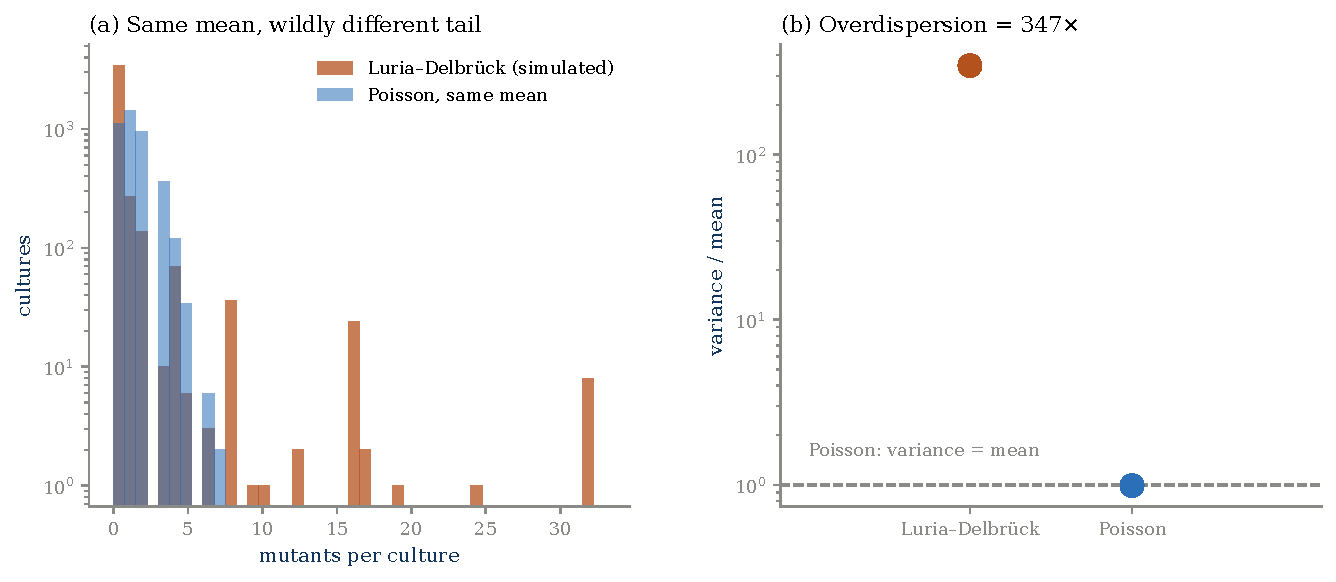
\includegraphics[width=\textwidth]{fig06_mutation_accumulation.pdf}
  \caption{(a) Simulated Luria--Delbrück counts against a Poisson distribution
  with the \emph{same mean}. The histograms are plotted on a logarithmic count
  axis; the Luria--Delbrück distribution places far more mass at zero and carries
  a tail the Poisson never reaches. (b) The variance-to-mean ratio. Each filled
  point is one reseed of the whole $4000$-culture experiment; the circled point
  is the seed quoted in the text. Every one of them falls far below the
  closed-form value (green), because $4000$ cultures cannot sample the
  first-generation events that carry the variance. The scatter, not any single
  point, is the honest summary --- see \S\ref{sub:trap}.}
  \label{fig:ld}
\end{figure}

\subsection{Consequences for Section~\ref{sec:refutation}}

Two points carry back to the refutation.

First, the rates in Table~\ref{tab:kane} are maximum-likelihood estimates from
fluctuation data, not sample means, which is why they are quoted without naive
standard errors and why their confidence intervals are asymmetric.

Second --- and this is why the ratio $\rho$ was the right statistic --- both
alleles were measured by the same protocol in the same background. Systematic
factors in the estimator (the growth model, the plating efficiency, the reporter
target size) enter both numerator and denominator and cancel. A comparison of
$\rho$ against a bound of $1$ is far more robust than either rate taken alone.

\begin{worked}[6.1: why the mode is zero]
\textbf{Problem.} With $\nu = 2\mu = 4\times10^{-8}$ and $N = 4.19\times10^{6}$,
the expected mutant count is $1.85$. Why do $85\%$ of cultures nevertheless
contain none?

\textbf{Solution.} The mean is carried by rare large clones. The total number of
wild-type divisions in a culture is $N - 1$, so the expected number of
mutational events anywhere in it is $\nu(N-1) = 0.168$, and if events are
approximately Poisson then
\[
  \Pr[\text{no event at all}] \;\approx\; e^{-0.168} \;=\; 0.845,
\]
against the simulated $0.854$. Meanwhile a single event $10$ generations from the
end contributes $2^{10} = 1024$ mutants by itself --- the observed maximum. A
distribution with most mass at zero and a mean above one must have a very heavy
tail, and that is exactly what \eqref{eq:ldvar} predicts.

Note the consistency check this provides, and what it does \emph{not} cover: the
zero-fraction is predicted to within $1\%$ because it depends only on the total
event count, a quantity $4000$ cultures sample well. The variance depends on
\emph{when} those events occur, which they sample badly. Two statistics from one
simulation, one trustworthy and one not.
\end{worked}

\begin{exercise}
Verify \eqref{eq:ldmean} by evaluating the sum directly for $g = 4$ and
$\nu = 10^{-2}$, and compare with $\tfrac{1}{2}\nu g N$.
\end{exercise}

\begin{exercise}
Show that for a Poisson random variable the variance-to-mean ratio is exactly~$1$,
and explain why any mechanism producing independent per-cell events at the moment
of challenge must give that ratio.
\end{exercise}

\begin{exercise}
The simulation uses synchronous doubling, which real cultures do not do. Argue
qualitatively whether asynchronous growth would increase or decrease the
overdispersion, and why the \emph{sign} of the Luria--Delbrück signature is robust
to this idealisation even though its magnitude is not.
\end{exercise}

\begin{exercise}[(harder)]
Suppose a variant raises $\nu$ by a factor $\rho$. Show that the \emph{ratio} of
mean mutant counts between variant and reference is $\rho$, independent of $g$
and $N$, provided both are grown identically. This is the cancellation that makes
$\rho$ in Section~\ref{sec:refutation} meaningful.
\end{exercise}

\begin{exercise}[(harder)]
Section~\ref{sub:trap} claims $4000$ cultures cannot estimate
$\operatorname{Var}[X]$. Make the claim quantitative. The variance is dominated
by events in the first few generations; require that a culture set contain, in
expectation, at least one generation-$0$ event, and deduce the number of
cultures needed at $\nu = 4\times10^{-8}$. Comment on whether the experiment is
feasible, and on what this implies for any published variance-to-mean ratio from
a fluctuation test.
\end{exercise}

\begin{ledger}
\textbf{Measured:} nothing new here; the section explains the estimator behind
the rates already quoted in Section~\ref{sec:refutation}. The simulated
quantities are computations, not measurements. \\
\textbf{Assumed:} Assumption~\ref{model:ld} --- synchronous doubling, neutral
non-reverting mutants, constant $\nu$ per cell per generation. All three are
idealisations. \\
\textbf{Proved:} nothing is formalised in this section. Equations
\eqref{eq:ldmean} and \eqref{eq:ldvar} are derived by hand. They are
\emph{not} confirmed by the simulation: \S\ref{sub:trap} shows the sample
variance falls short of \eqref{eq:ldvar} by a factor of about $550$ for a reason
the model itself explains. The mean agrees to within sampling error; the variance
is not testable at $4000$ cultures. \\
\textbf{Open:} the asynchronous-growth correction of Exercise~6.3 is not computed
anywhere in this book. Neither is the number of cultures that \emph{would} make
the variance estimable --- Exercise~6.5 asks for the order of magnitude, and it
is large enough to be a real obstacle to using this statistic at all. \\
\textbf{Corrected in this edition:} the first edition quoted the single-seed
variance-to-mean ratio of $346.7$ as the section's result, beside a closed form
predicting $190\,650$, without reconciling them or reporting that reseeding moves
the number by seventy-fold. See \S\ref{sub:trap}.
\end{ledger}

% =============================================================================
% Section 7 — Variant Landscapes from Live Databases
% =============================================================================
\section{Variant Landscapes: What the Databases Actually Say}\label{sec:variants}

\begin{objectives}
\begin{itemize}[leftmargin=*,itemsep=1pt,topsep=1pt]
  \item Retrieve gene, protein and variant records from Ensembl, UniProt, InterPro and ClinVar.
  \item Locate a variant within a protein domain and verify the claim rather than assert it.
  \item Read ClinVar base rates correctly, including why its categories do not partition.
  \item Recognise the reference-assembly and overlap pitfalls that corrupt variant arguments.
\end{itemize}
\end{objectives}

\subsection{Why retrieve rather than quote}

Every identifier in this book is fetched from a public endpoint and cached with
its URL and a UTC timestamp, by
\file{scripts/textbook/retrieve_genomic_data.py}. There are two reasons, and the
second is the important one.

The obvious reason is reproducibility. The deeper reason is that \emph{retrieval
can fail a claim}. When the script is run, it checks its own output: that every
gene record is on GRCh38, that every domain lies inside its protein, and that
residue $286$ falls within the retrieved boundaries of \texttt{IPR006133}. If any
check fails it refuses to write the cache. An assertion in prose cannot do that.

\subsection{What the records say}

\begin{table}[htbp]
\centering
\caption{Gene records retrieved from Ensembl REST, GRCh38. The replicative
polymerases of Sections~\ref{sec:proofreading}--\ref{sec:refutation} and the
mismatch-repair genes of Section~\ref{sec:mmr}.}
\label{tab:genes}
\begin{tabularx}{\linewidth}{@{}l l r r X@{}}
\toprule
\textbf{Gene} & \textbf{Ensembl ID} & \textbf{Chr} & \textbf{Span (bp)} & \textbf{Role here} \\
\midrule
\texttt{POLE}  & \texttt{ENSG00000177084} & 12 & $63\,624$  & leading-strand polymerase; the variant \\
\texttt{POLD1} & \texttt{ENSG00000062822} & 19 & $33\,815$  & lagging-strand polymerase; comparison \\
\texttt{MSH6}  & \texttt{ENSG00000116062} & 2  & $114\,580$ & MMR recognition; the $\textsf{msh6}\Delta$ of §\ref{sec:mmr} \\
\texttt{MSH2}  & \texttt{ENSG00000095002} & 2  & $260\,080$ & MMR recognition partner \\
\texttt{MLH1}  & \texttt{ENSG00000076242} & 3  & $58\,672$  & MMR effector \\
\bottomrule
\end{tabularx}
\end{table}

The protein picture is where the argument of Section~\ref{sec:refutation} is
anchored. \texttt{POLE} (UniProt \texttt{Q07864}) is $2286$ residues. InterPro
places five domains on it; the one that matters is \texttt{IPR006133}, the
family-B DNA polymerase exonuclease domain, at residues $220$--$426$.

\begin{figure}[htbp]
  \centering
  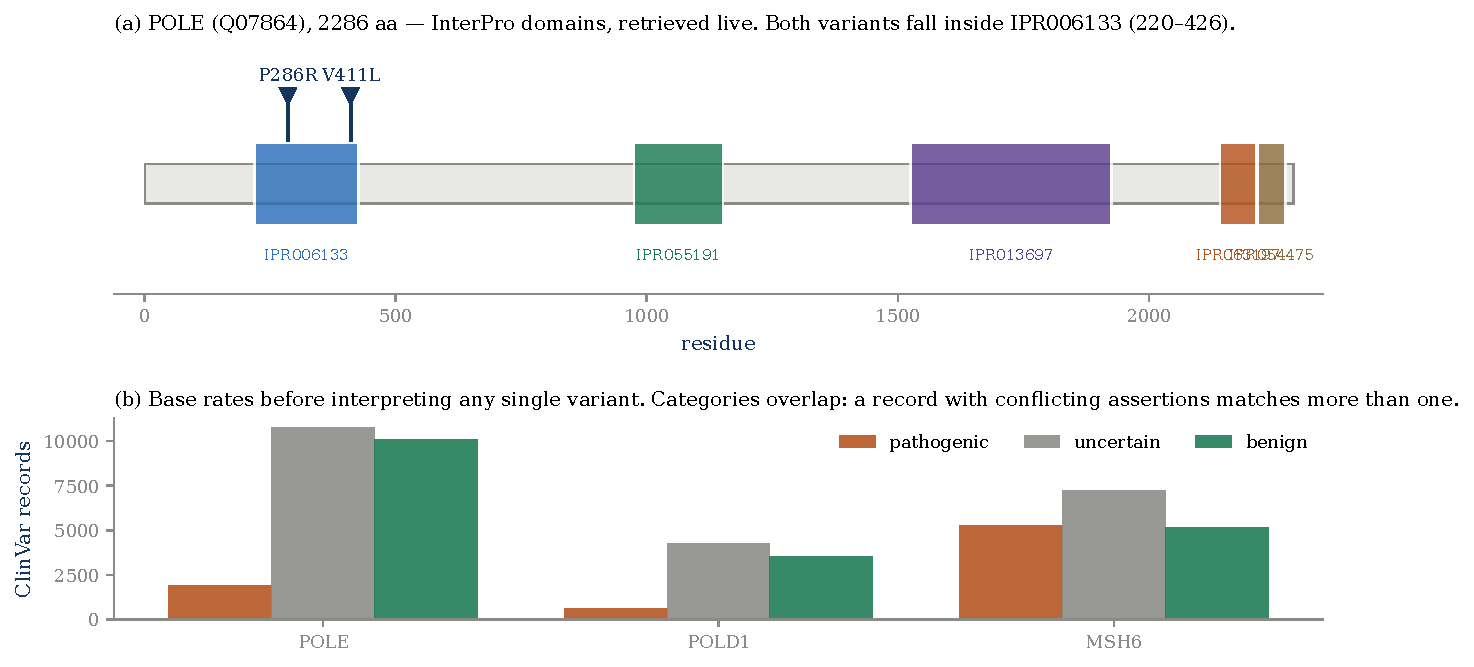
\includegraphics[width=\textwidth]{fig07_variant_landscape.pdf}
  \caption{(a) \texttt{POLE} domain architecture from InterPro, drawn to scale,
  with the two variants discussed in this book marked. Both \texttt{P286R} and
  the neutral control \texttt{V411L} fall inside the exonuclease domain --- which
  is itself instructive: being in the proofreading domain does not make a variant
  a mutator, as Section~\ref{sec:refutation}'s control shows. (b) ClinVar record
  counts. Note that the categories overlap.}
  \label{fig:landscape}
\end{figure}

\subsection{Reading ClinVar without being misled}

Figure~\ref{fig:landscape}(b) reports, for \texttt{POLE}: $1891$ records matching
``pathogenic'', $10\,065$ matching ``benign'', $10\,737$ matching ``uncertain
significance'', against $11\,341$ records in total.

Those numbers sum to $22\,693$, twice the total. This is not an error in the
retrieval, and the fact is worth dwelling on because it trips people up
constantly: \textbf{ClinVar's clinical-significance categories do not partition
the records}. A variant with conflicting submissions matches more than one
filter. Any argument of the form ``$x\%$ of variants in this gene are pathogenic,
computed as pathogenic over total'' is therefore wrong.

\begin{remark}[The base-rate discipline]
Before interpreting any individual variant, look at the gene's base rates.
\texttt{POLE} has $1891$ pathogenic-matching records against $10\,737$ of
uncertain significance. The modal outcome of finding a novel \texttt{POLE}
missense variant in a patient is \emph{not} a diagnosis; it is a VUS. A method
that confidently classifies such variants should be viewed against that base
rate, not against its own accuracy on curated examples.
\end{remark}

\begin{worked}[7.1: a variant in the right domain that does nothing]
\textbf{Problem.} \texttt{V411L} lies at residue $411$, inside \texttt{IPR006133}
($220$--$426$), the same domain as \texttt{P286R}. Yet Section~\ref{sec:refutation}
used it as a \emph{negative} control: it does not break the PSR$_2$ ceiling. Is
this a contradiction?

\textbf{Solution.} No, and the apparent tension is the point of the exercise.
Domain membership is a statement about \emph{where} a residue sits in a sequence
annotation; mutator phenotype is a statement about \emph{what} the substituted
protein does. Localisation is evidence of opportunity, not of effect.

Concretely: the exonuclease domain contains catalytic residues, metal-coordinating
residues, structural residues and surface residues. A substitution at a surface
position inside the domain may leave catalysis untouched. Inferring function from
domain membership is the same category error that Section~\ref{sec:proof-and-cell}
warned about --- treating a modelling claim (``in the domain, therefore disrupts
the domain'') as though it were established.
\end{worked}

\begin{exercise}
Using Table~\ref{tab:genes}, compute the genomic span of \texttt{MSH2} in
kilobases and compare it with \texttt{POLE}. Does a larger gene imply more
ClinVar records? Check against Figure~\ref{fig:landscape}(b) and comment.
\end{exercise}

\begin{exercise}
A colleague computes ``the pathogenic fraction of \texttt{MSH6}'' as
$5289/10\,849 = 48.8\%$ and concludes that \texttt{MSH6} variants are more often
pathogenic than not. Identify two independent errors in this reasoning.
\end{exercise}

\begin{exercise}
The retrieval script asserts that every gene record carries
\texttt{assembly == "GRCh38"}. Explain what could go wrong in a variant analysis
if records from GRCh37 and GRCh38 were mixed, and why a coordinate alone is not
a variant identifier.
\end{exercise}

\begin{exercise}[(harder)]
Section~\ref{sec:refutation} relies on the yeast allele \texttt{pol2-P301R} being
the analogue of human \texttt{P286R}. Using the UniProt and InterPro records,
describe the evidence you would need to justify that correspondence, and state
what the argument assumes that the databases do not supply.
\end{exercise}

\begin{ledger}
\textbf{Measured:} all records in Table~\ref{tab:genes} and
Figure~\ref{fig:landscape}, retrieved live from Ensembl REST, UniProt, InterPro
and NCBI E-utilities; URLs and timestamps in
\file{textbook/data/genomic_records.json}. \\
\textbf{Assumed:} that the canonical/MANE transcript is the appropriate
coordinate frame, and that InterPro domain boundaries are an adequate proxy for
functional boundaries. The second is weaker than it looks --- see
Worked Example~7.1. \\
\textbf{Proved:} nothing formalised. The retrieval script's internal consistency
checks are assertions over fetched data, not theorems: they can fail at runtime,
which is their purpose. \\
\textbf{Open:} the yeast-to-human correspondence of Exercise~7.4 is assumed
throughout this book and is nowhere established in it.
\end{ledger}

% =============================================================================
% Section 8 — Topological Data Analysis of Genomic Sequence
% =============================================================================
\section{Topology of a Genome: Persistent Homology on Real Sequence}\label{sec:tda}

\begin{objectives}
\begin{itemize}[leftmargin=*,itemsep=1pt,topsep=1pt]
  \item Embed a DNA sequence as a point cloud whose geometry encodes $k$-mer context.
  \item Define a filtration and read birth--death pairs from a persistence diagram.
  \item Compute Betti numbers on a real coding sequence with GUDHI.
  \item Judge honestly when a topological feature is signal and when it is an artefact of the embedding.
\end{itemize}
\end{objectives}

\subsection{Why topology, and when not}

Topological data analysis asks what shape a dataset has at every scale at once.
Applied carelessly to biology it produces impressive pictures and no knowledge,
so this section is as much about restraint as about method. We compute real
persistent homology on a real sequence, and then we ask what it establishes ---
and the honest answer turns out to be narrower than the picture suggests.

\subsection{From sequence to point cloud}

A sequence of letters has no geometry until we give it one. The classical device
is the \textbf{chaos game representation}.

\begin{definition}[Chaos game representation, 3D]\label{def:cgr}
Assign the four bases to the vertices of a regular tetrahedron,
$v_A, v_C, v_G, v_T \in \mathbb{R}^3$. Start at the origin, $x_0 = 0$, and for
each successive base $b_i$ set
\begin{equation}\label{eq:cgr}
  x_i \;=\; \tfrac{1}{2}\left(x_{i-1} + v_{b_i}\right).
\end{equation}
\end{definition}

The construction has a property that makes it useful rather than decorative:
after $k$ steps the influence of $x_{i-k}$ is scaled by $2^{-k}$. Two positions
in the sequence therefore land close together exactly when they share a recent
suffix. Proximity in the cloud \emph{is} shared $k$-mer context, with longer
shared context giving closer points. The embedding is not arbitrary; it is a
geometric encoding of word statistics.

\subsection{Filtration and persistence}

\begin{definition}[Vietoris--Rips filtration]
For a finite point set $X \subset \mathbb{R}^3$ and $\epsilon \ge 0$, the complex
$\mathrm{VR}_\epsilon(X)$ has a simplex on every subset of diameter at most
$\epsilon$. As $\epsilon$ grows the complexes nest, and a homology class born at
$\epsilon_b$ and dying at $\epsilon_d$ is recorded as the pair
$(\epsilon_b, \epsilon_d)$.
\end{definition}

The quantity $\epsilon_d - \epsilon_b$ is the feature's \emph{persistence}. The
working assumption of TDA is that long bars are structure and short bars are
noise. That assumption is exactly what needs checking in any application.

\subsection{Computation on the \texttt{POLE} coding sequence}

\begin{numerics}[8.1]
\file{scripts/textbook/make_figures.py}, section~8. The canonical \texttt{POLE}
coding sequence is fetched from Ensembl ($6861$~nt), embedded by
\eqref{eq:cgr}, and subsampled to $900$ points. Persistent homology is computed
with GUDHI~3.13.0, Vietoris--Rips, maximum edge length $0.9$, up to dimension~2.

\medskip
\begin{tabularx}{\linewidth}{@{}l r X@{}}
\toprule
coding sequence length & $6861$ nt & Ensembl canonical transcript \\
points after subsampling & $900$ & uniform stride \\
Betti numbers $(\beta_0, \beta_1)$ & $(1, 0)$ & at the filtration limit \\
longest $H_1$ bar & $(0.171,\ 0.755)$ & persistence $0.584$ \\
\bottomrule
\end{tabularx}
\end{numerics}

\begin{figure}[htbp]
  \centering
  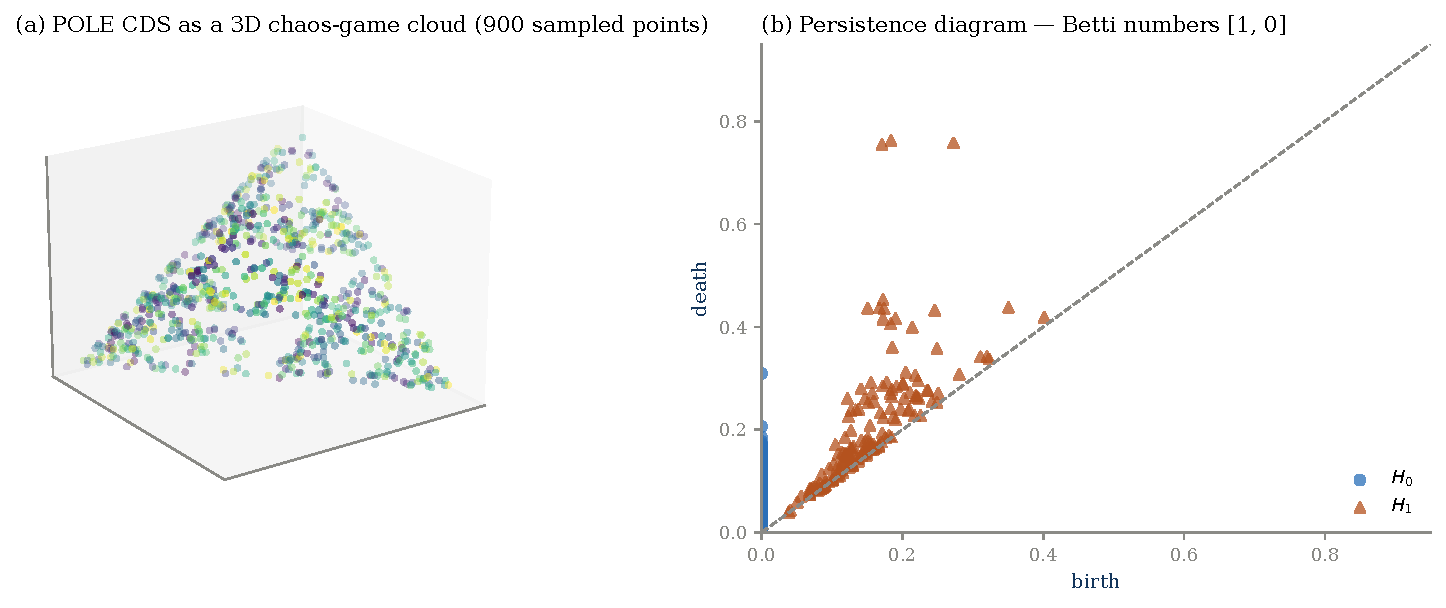
\includegraphics[width=\textwidth]{fig08_topological_genomics.pdf}
  \caption{(a) The \texttt{POLE} coding sequence as a chaos-game point cloud in
  $\mathbb{R}^3$, coloured by position along the transcript. The tetrahedral
  self-similar structure is the signature of \eqref{eq:cgr}. (b) The persistence
  diagram. Points far from the diagonal are long-lived features; $H_1$ classes
  are born and die well inside the filtration, leaving $\beta_1 = 0$ at the limit.}
  \label{fig:tda}
\end{figure}

\subsection{Reading the result honestly}

The cloud is connected ($\beta_0 = 1$) and has no surviving loops
($\beta_1 = 0$). There are, however, $H_1$ classes of substantial persistence ---
the longest living from $\epsilon = 0.171$ to $\epsilon = 0.755$.

Now the question that matters: \emph{is that a fact about \texttt{POLE}?}

It is largely a fact about the chaos game. The map \eqref{eq:cgr} sends any
sequence into a self-similar attractor --- the tetrahedral Sierpiński gasket ---
whose holes exist regardless of what the sequence says. A random sequence
produces loops of comparable persistence. So the bare Betti numbers of a single
sequence carry almost no biological information, and reporting them as though
they did would be precisely the overclaiming this book is organised against.

\begin{remark}[What would make this informative]
TDA becomes informative here under \emph{comparison}, not in isolation. The
honest designs are:
\begin{enumerate}[leftmargin=*,itemsep=1pt]
  \item \textbf{Against a null.} Compare the persistence of the real sequence
        with an ensemble of shuffles preserving mononucleotide --- or better,
        dinucleotide --- composition. A feature is evidence only if it exceeds
        that null.
  \item \textbf{Between sequences.} Compare persistence landscapes of orthologous
        genes, or of coding against non-coding regions, where the embedding
        artefact is common to both and cancels.
\end{enumerate}
This book computes neither. Figure~\ref{fig:tda} is therefore offered as a
\emph{method demonstration}, and the ledger records it as such. A reader who
wanted a biological claim from TDA should regard this section as the setup, not
the result.
\end{remark}

\begin{worked}[8.1: why the subsampling stride matters]
\textbf{Problem.} The computation subsamples $6861$ points down to $900$ by
uniform stride. Why not use all points, and what does the stride risk?

\textbf{Solution.} Vietoris--Rips on $n$ points builds up to $\binom{n}{3}$
triangles at dimension~2; at $n = 6861$ that is $5\times10^{10}$ simplices, which
is not computable here. Subsampling is a necessity, not a refinement.

The risk is specific: a uniform stride of $7$ interacts with the codon structure
of a coding sequence, whose period is $3$. A stride sharing a factor with the
reading frame can systematically over-sample one codon position. Here
$\gcd(7, 3) = 1$, so the three positions are sampled evenly --- but the check is
necessary, and a stride of $6$ or $9$ would have introduced a frame bias
invisible in the final diagram. Artefacts of this kind are the normal failure
mode of applied topology.
\end{worked}

\begin{exercise}
Show from \eqref{eq:cgr} that $x_i$ depends on $b_{i-k}$ with weight $2^{-k}$,
and deduce that two positions sharing a suffix of length $k$ lie within
$2^{-k}\,\mathrm{diam}$ of each other.
\end{exercise}

\begin{exercise}
Explain why $\beta_0 = 1$ at the filtration limit is uninformative for any
sufficiently long sequence. What value of the maximum edge length would make
$\beta_0$ informative, and what would it then be measuring?
\end{exercise}

\begin{exercise}
Design the shuffle null described in the remark. State precisely what is
preserved by your shuffle and what is destroyed, and say which biological
hypothesis each choice would let you test.
\end{exercise}

\begin{exercise}[(harder)]
Persistence diagrams can be compared with the bottleneck distance. Look up its
definition and explain why it is stable --- small perturbations of the point
cloud produce small changes in the diagram. Why is that stability a prerequisite
for using TDA on noisy biological data at all?
\end{exercise}

\begin{ledger}
\textbf{Measured:} the \texttt{POLE} canonical coding sequence, $6861$~nt,
retrieved from Ensembl and cached with its URL. The persistence computation is
exact given the point cloud (GUDHI~3.13.0). \\
\textbf{Assumed:} that the chaos-game embedding is a meaningful geometry for
sequence, and that Vietoris--Rips persistence on a $900$-point subsample
represents the full cloud. \\
\textbf{Proved:} nothing formalised. The Betti numbers are a computation, not a
theorem, and they are reported as a method demonstration. \\
\textbf{Open:} everything that would make this biological --- the shuffle null,
the cross-sequence comparison. Neither is performed in this book, and no claim
about \texttt{POLE} should be drawn from Figure~\ref{fig:tda}.
\end{ledger}

% =============================================================================
% Section 9 — DNA Topology
% =============================================================================
\section{DNA Topology: Linking, Twist and Writhe}\label{sec:dnatop}

\begin{objectives}
\begin{itemize}[leftmargin=*,itemsep=1pt,topsep=1pt]
  \item State the Călugăreanu--White--Fuller theorem and identify which of its terms are topological.
  \item Prove that conserved linking forces an exact trade between twist and writhe.
  \item Explain why replication creates a topological problem that no amount of force can solve.
  \item Connect supercoiling to the polymerase fidelity of Sections~\ref{sec:proofreading}--\ref{sec:refutation}.
\end{itemize}
\end{objectives}

\subsection{Biological setting}

A replication fork unwinds the double helix at roughly $50$ base pairs per
second. Because the two strands are wound about each other, unwinding them
requires either rotating the entire chromosome ahead of the fork --- impossible
for a molecule of that length --- or storing the rotation as strain in the DNA
itself. The cell does the latter, then relieves the strain with topoisomerases.

The mathematics that describes this storage is not an analogy. It is a theorem
about closed ribbons, and the quantity it conserves is an integer.

\subsection{How the helix was established: reading Photo 51}\label{sub:photo51}

Before modelling the geometry we should ask how it is known, and the answer is a
diffraction pattern. A helix of radius $r$ and pitch $P$, illuminated along a
direction perpendicular to its axis, produces a transform given by the
Cochran--Crick--Vand theory: on the layer line indexed by $n$, at height
$Z = n/P$ in reciprocal space, the amplitude is
\begin{equation}\label{eq:ccv}
  F_n(R) \;\propto\; J_n\!\left(2\pi r R\right),
\end{equation}
with $J_n$ the Bessel function of the first kind. The maxima of successive $J_n$
move outward with $n$, and the locus of those maxima is the famous \emph{X}. Its
opening angle gives $P/r$ directly.

For a \emph{double} helix the two strands are offset along the axis by a fraction
$\delta$ of the pitch, and their contributions interfere:
\begin{equation}\label{eq:interf}
  I_n(R) \;\propto\; \left|J_n(2\pi r R)\right|^{2}\cdot 4\cos^{2}\!\left(\pi n \delta\right).
\end{equation}
Now take the B-DNA value $\delta = 3/8$, which is what the minor- and major-groove
widths amount to. At $n = 4$,
\[
  \cos\!\left(\pi \cdot 4 \cdot \tfrac{3}{8}\right) = \cos\!\left(\tfrac{3\pi}{2}\right) = 0,
\]
and the fourth layer line vanishes identically. A systematic absence of this kind
is not a weak feature to be argued over; it is a yes-or-no observation, and it is
present in Photo~51.

\begin{figure}[htbp]
  \centering
  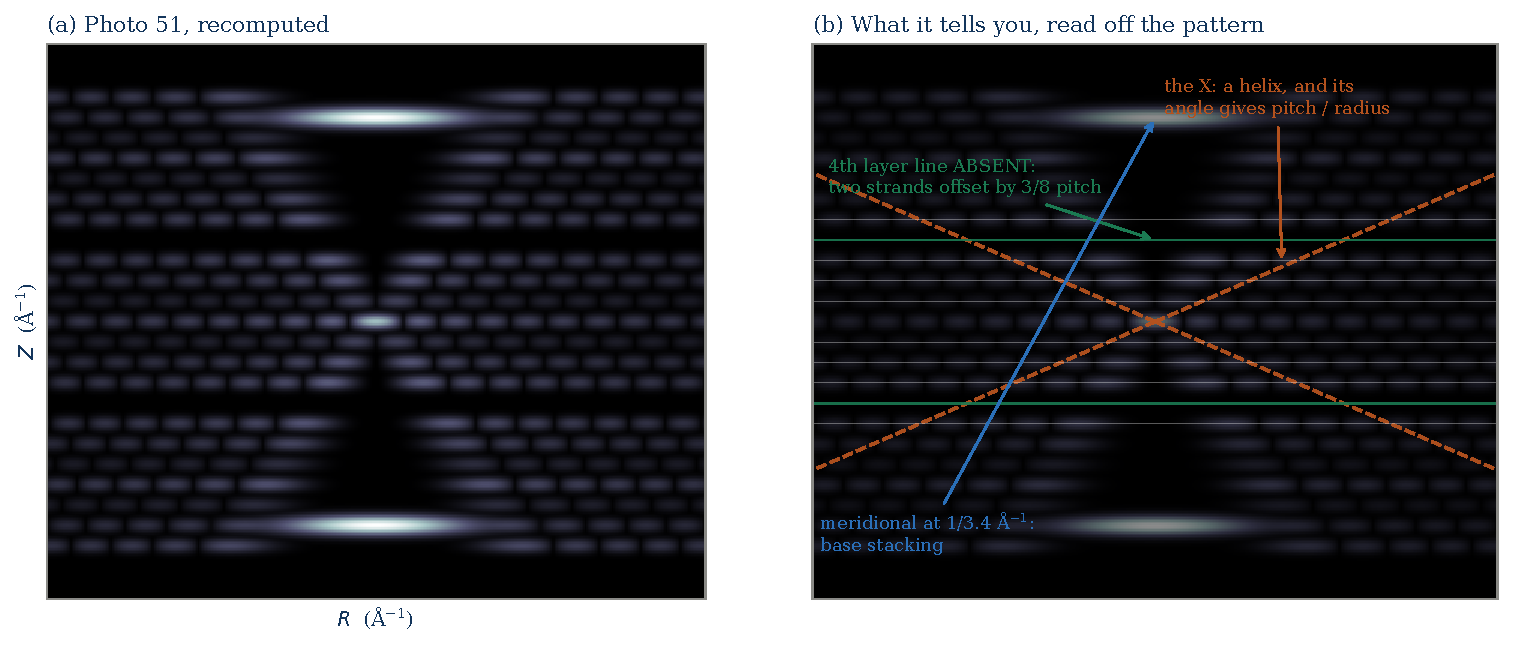
\includegraphics[width=\textwidth]{fig00_photo51.pdf}
  \caption{Photo~51, recomputed from \eqref{eq:ccv} and \eqref{eq:interf} with
  B-DNA parameters ($r = 10$\,\AA, $P = 34$\,\AA, rise $3.4$\,\AA,
  $\delta = 3/8$). This is not a traced copy of the plate: the features are
  outputs of the transform. (a) The pattern. (b) What it determines --- the helix
  cross fixing $P/r$, the meridional at $1/3.4\,\text{\AA}^{-1}$ from base
  stacking, and the fourth layer line (green) absent because
  $\cos(3\pi/2) = 0$. Generated by \file{scripts/textbook/make_figures.py}.}
  \label{fig:photo51}
\end{figure}

\begin{remark}[Why this belongs in a book about formal methods]
Equation~\eqref{eq:interf} is a derivation with no adjustable parameter at the
point that matters: given a two-strand helix with $\delta = 3/8$, the fourth
layer line \emph{must} be absent. This is the same logical shape as PSR$_2$ in
Section~\ref{sec:nogo} --- a parameter-free consequence, sharp enough that a
single observation decides it. Franklin's photograph was evidential precisely
because the structure it supported made a prediction that could have failed and
did not. The epistemics of 1952 and of this book are the same epistemics.
\end{remark}

\subsection{Mathematical development}

Model duplex DNA as a \emph{ribbon}: a closed space curve $C$ (the axis) together
with a unit normal field $u$ along it (pointing to one backbone). Three numbers
describe it.

\begin{definition}[Linking, twist, writhe]\label{def:lktwwr}
\begin{itemize}[leftmargin=*,itemsep=1pt,topsep=1pt]
  \item $\Lk$, the \textbf{linking number}, counts the signed crossings between
        the two edges of the ribbon. It is an \emph{integer} and a topological
        invariant: it cannot change under any deformation that does not cut a strand.
  \item $\Tw$, the \textbf{twist}, measures the rotation of $u$ about $C$,
        integrated along the curve. It is a real number and depends on geometry.
  \item $\Wr$, the \textbf{writhe}, measures the coiling of the axis $C$ in space,
        averaged over all viewing directions. It too is real and geometric.
\end{itemize}
\end{definition}

\begin{theorem}[Călugăreanu--White--Fuller]\label{thm:cwf}
For a closed ribbon, $\;\Lk = \Tw + \Wr$.
\end{theorem}

We do not prove this here --- it is a theorem of differential geometry, and the
proof would take the section far from biology. What we do prove is the
consequence that does the biological work.

\begin{theorem}[Twist--writhe trade-off]\label{thm:trade}
Suppose a segment is deformed between two states with the linking number
conserved, $\Lk_1 = \Lk_2 = \Lk$. Then
\[
  \Tw_2 - \Tw_1 \;=\; -\left(\Wr_2 - \Wr_1\right).
\]
Every turn of twist released by the helix reappears exactly as writhe of the axis.
\end{theorem}

\begin{proof}
By Theorem~\ref{thm:cwf}, $\Lk = \Tw_1 + \Wr_1$ and $\Lk = \Tw_2 + \Wr_2$.
Subtracting, $0 = (\Tw_2 - \Tw_1) + (\Wr_2 - \Wr_1)$.
\end{proof}

The content is in the \emph{exactness}. Strain is not dissipated by deforming the
molecule; it is only moved between two reservoirs. A cell cannot relax
supercoiling by wiggling. It must cut a strand --- which is what topoisomerases
do, and why they are essential genes and major drug targets.

\subsection{Formalisation}

In \file{formal/ANSE/GeneticsTextbook.lean}.

\begin{lstlisting}
theorem linking_conserved_twist_writhe (Lk Tw₁ Wr₁ Tw₂ Wr₂ : ℝ)
    (h₁ : Lk = Tw₁ + Wr₁) (h₂ : Lk = Tw₂ + Wr₂) :
    Tw₂ - Tw₁ = -(Wr₂ - Wr₁) := by linarith
\end{lstlisting}

The proof is one tactic, and it is worth being explicit about why so trivial a
formalisation is nevertheless worth having. What the Lean statement pins down is
the \emph{hypothesis structure}: the conclusion needs $\Lk$ to be the same number
in both equations, and nothing else. The companion
\lean{twist_writhe_needs_conservation} exhibits a pair of states where linking is
not conserved and the trade-off fails, confirming the hypothesis is load-bearing.
Formalising a triviality has no value; formalising which hypothesis a triviality
rests on sometimes does.

\begin{figure}[htbp]
  \centering
  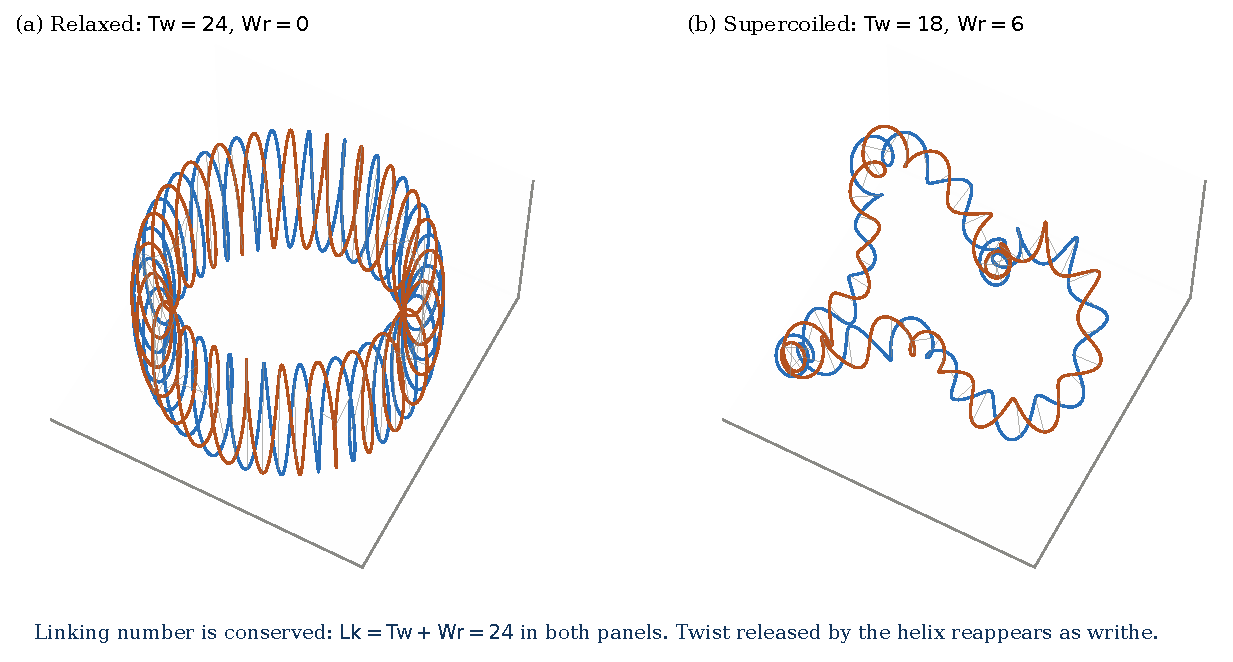
\includegraphics[width=\textwidth]{fig09_dna_topology.pdf}
  \caption{Two states of the same closed duplex at $\Lk = 24$. (a) Relaxed: all
  $24$ turns are twist, the axis is planar, $\Wr = 0$. (b) Supercoiled: six turns
  have been converted to writhe, the axis coils in space, $\Tw = 18$. The linking
  number --- the only topological quantity of the three --- is identical. Generated
  by \file{scripts/textbook/make_figures.py}, section~9.}
  \label{fig:supercoil}
\end{figure}

\subsection{Back to fidelity}

This section connects to the rest of the book through torque. A polymerase
elongating against accumulated positive supercoiling works against a mechanical
load, and the Bell--Kramers picture says a load modifies kinetic barriers
exponentially:
\begin{equation}\label{eq:bell}
  \gamma(\Gamma) \;=\; \gamma_0 \exp\!\left(\beta_{\mathrm{tor}}\Gamma\right).
\end{equation}
If torque raises the per-stage escape probability $\gamma$, then by
Proposition~\ref{prop:gain} the error rate rises geometrically in the number of
stages affected.

That is a hypothesis, not a result, and this book does not test it. It is
recorded here because it is the kind of coupling a student should notice: the
topological state of the template is a candidate input to the fidelity models of
Section~\ref{sec:proofreading}, and \eqref{eq:bell} would let it in through
$\gamma$ rather than through the repair capacity $c$ of Section~\ref{sec:mmr}.
Distinguishing those two routes experimentally would be a genuine contribution.

\begin{worked}[9.1: counting turns in a plasmid]
\textbf{Problem.} A relaxed circular plasmid of $3600$ bp has $\Lk_0 = 3600/10.5
\approx 343$ turns. A topoisomerase removes $17$ turns. If the resulting molecule
adopts a conformation with $\Wr = -14$, what is its twist, and what is the
superhelical density?

\textbf{Solution.} After the enzyme acts, $\Lk = 343 - 17 = 326$. By
Theorem~\ref{thm:cwf}, $\Tw = \Lk - \Wr = 326 - (-14) = 340$. The helix is
therefore still close to its relaxed twist of $343$, with most of the deficit
absorbed as negative writhe --- which is the usual outcome, because bending the
axis is energetically cheaper than over- or under-winding the helix.

The superhelical density is
$\sigma = (\Lk - \Lk_0)/\Lk_0 = -17/343 \approx -0.050$, close to the $\sigma
\approx -0.06$ typical of bacterial plasmids in vivo.
\end{worked}

\begin{exercise}
Using Theorem~\ref{thm:trade}, show that if a protein locally unwinds one turn of
helix ($\Delta\Tw = -1$) in a topologically closed domain, the compensating
writhe is exactly $+1$. Where does that writhe go physically?
\end{exercise}

\begin{exercise}
$\Lk$ is an integer; $\Tw$ and $\Wr$ are not. Explain how a sum of two
non-integers is forced to be an integer, and what breaks if the ribbon is not
closed.
\end{exercise}

\begin{exercise}
A replication fork advancing $1000$ bp introduces roughly $1000/10.5 \approx 95$
turns of positive supercoiling ahead of it. At $50$ bp/s, how many turns per
second must topoisomerase remove to keep the template relaxed?
\end{exercise}

\begin{exercise}[(harder)]
Using \eqref{eq:bell} and Proposition~\ref{prop:gain}, derive how the three-stage
error rate $\gamma(\Gamma)^3$ depends on torque, and state the measurement that
would test it. Why is it difficult to separate this from the repair-capacity
mechanism of Section~\ref{sec:mmr}?
\end{exercise}

\begin{ledger}
\textbf{Measured:} nothing in this section. The plasmid numbers in Worked
Example~9.1 are illustrative, chosen to match typical bacterial superhelical
densities; they are not a reported measurement. \\
\textbf{Assumed:} the ribbon model of duplex DNA, closure of the topological
domain, and --- for \eqref{eq:bell} --- a Bell--Kramers response of the kinetic
barrier to torque. The last is a hypothesis this book does not test. \\
\textbf{Proved:} Theorem~\ref{thm:trade} (\lean{linking_conserved_twist_writhe}),
with the control \lean{twist_writhe_needs_conservation}. Theorem~\ref{thm:cwf} is
cited, not proved, and is not formalised. \\
\textbf{Open:} whether template supercoiling contributes measurably to the
fidelity defects of Section~\ref{sec:refutation}, and whether that contribution
could be distinguished from a repair-capacity effect.
\end{ledger}

% =============================================================================
% Section 10 — From Model to Clinic
% =============================================================================
\section{From Model to Clinic: What Survives, and What Humanity Gains}\label{sec:clinic}

\begin{objectives}
\begin{itemize}[leftmargin=*,itemsep=1pt,topsep=1pt]
  \item Trace which clinical conclusions survive the refutation of their supporting mechanism.
  \item Distinguish a therapeutic decision rule from the model once used to motivate it.
  \item State what formal methods contribute to medicine, and what they do not.
  \item Assess honestly what this book's programme offers and what it costs.
\end{itemize}
\end{objectives}

\subsection{The clinical fact}

Tumours carrying proofreading-domain \texttt{POLE} mutations are among the most
heavily mutated in oncology. A high tumour mutational burden (TMB) means many
neoantigens, which means a tumour visible to the immune system, which is why
such tumours respond well to checkpoint inhibition. Pembrolizumab is approved
for TMB-high solid tumours at a threshold of $\ge 10$ mutations per megabase.

This is a clinical fact, established by measuring mutation burden in patient
tumours and observing response. It does not depend on any model in this book.

\subsection{What the retracted model predicted}

Earlier editions of this material derived the TMB of a \texttt{P286R} tumour from
the stage-removal model. With $\gamma = 3/250$ and a wild-type burden of
$0.2$ mut/Mb, dropping from $m = 3$ to $m = 1$ multiplies by $1/\gamma^{2} =
62\,500/9$, giving
\begin{equation}\label{eq:tmbpred}
  \TMB_{\text{P286R}} \;=\; \tfrac{1}{5}\cdot\tfrac{62500}{9} \;=\; \tfrac{12500}{9} \;\approx\; 1388.9 \ \text{mut/Mb}.
\end{equation}
The arithmetic is exact, and Lean will confirm it. The mechanism it rests on was
refuted in Section~\ref{sec:refutation}.

So what is \eqref{eq:tmbpred} worth? As a prediction, nothing: it is the output
of a model we have shown to be false. As an illustration of a ratio computation,
it is fine. The honest handling is to keep it, label it, and never cite it as a
clinical quantity --- which is what Figure~\ref{fig:clinic}(a) does.

\begin{figure}[htbp]
  \centering
  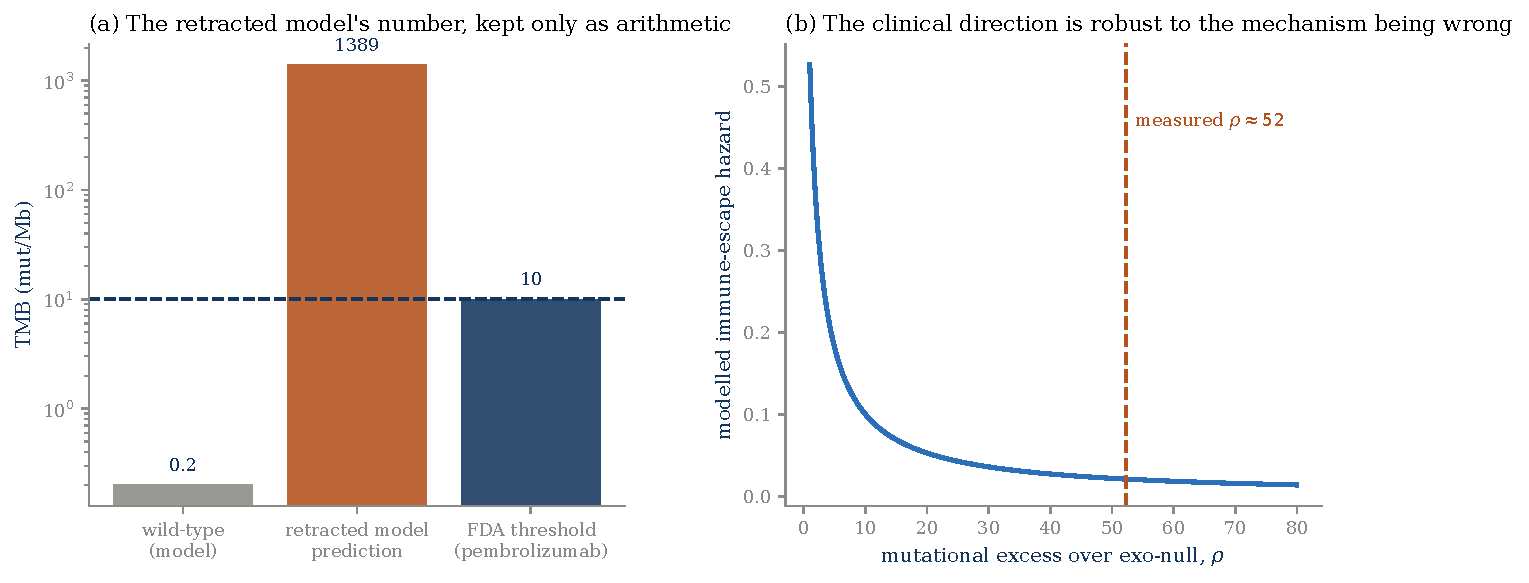
\includegraphics[width=\textwidth]{fig10_clinic.pdf}
  \caption{(a) The retracted model's prediction against the regulatory threshold,
  on a logarithmic axis. The bar is shown because deleting an error is worse
  pedagogy than displaying it, but it is arithmetic about a refuted model and not
  a claim about patients. (b) A modelled immune-escape hazard falling with
  mutational excess. The \emph{direction} of the clinical conclusion is robust:
  it does not depend on the mechanism that generates the excess.}
  \label{fig:clinic}
\end{figure}

\subsection{Why the clinical conclusion survives}

This is the most important distinction in the section, and it generalises well
beyond \texttt{POLE}.

The therapeutic decision rule is: \emph{measure TMB; if it exceeds $10$ mut/Mb,
consider checkpoint inhibition}. That rule takes TMB as an \emph{input}. It never
asks why the burden is high. A tumour mutated because proofreading failed, or
because repair was overwhelmed, or for a reason nobody has yet identified, enters
the rule identically.

The refuted model was never load-bearing for the clinic. It was an explanation
offered alongside a decision rule that measures the relevant quantity directly.
Refuting the explanation leaves the rule untouched.

\begin{remark}[The general pattern]
Clinical practice is often more robust than the mechanistic stories told around
it, because practice tends to measure the proximate quantity while stories
explain it. This is worth knowing in both directions. It means a refutation like
Section~\ref{sec:refutation}'s does not endanger patients --- but it also means a
mechanistic story that \emph{sounds} explanatory may be contributing nothing, and
its falsity may go unnoticed for years precisely because nothing downstream
depends on it. Ours went unnoticed for exactly that reason.
\end{remark}

\subsection{What formal methods are for in medicine}

It would be easy to end a book like this by claiming that machine-checked proof
will make biomedical science reliable. That claim would be false, and this book's
own history refutes it: every theorem in the retracted material passed the axiom
gate. The proofs were correct. The biology was wrong.

What formalisation did contribute is narrower and real:

\begin{enumerate}[leftmargin=*,itemsep=2pt]
  \item \textbf{It forced the hypothesis to be stated.} ``P286R removes
        proofreading stages'' became Assumption~\ref{model:class}, with an
        explicit domain and explicit ranges.
  \item \textbf{It made the hypothesis checkable.} Once stated that precisely,
        PSR$_2$ followed --- and PSR$_2$ had no free parameters, so a single
        ratio could kill it.
  \item \textbf{It located the replacement.} Theorem~\ref{thm:forced} does not
        guess at an interaction with repair; it derives one from two
        measurements.
\end{enumerate}

The contribution is \emph{exposure}, not certainty. A vague mechanism survives
indefinitely because nothing can contradict it. A formalised one can be killed by
one number, and ours was.

\subsection{The benefit to humanity, stated carefully}

The honest version of the humanitarian claim is modest and, we think, more
valuable for being modest.

Mechanistic errors in biomedical literature are common and persistent. They
persist because mechanisms are usually stated loosely enough to accommodate
contrary data. The practice this book demonstrates --- state the mechanism as a
model class, prove what the class entails without fitting, compare against a
directly measured reference, and publish the refutation when it comes --- is
transferable to any mechanistic claim in biology. It requires no new technology.
It requires being willing to write down what you believe precisely enough that it
can be shown wrong, and then to say so when it is.

The direct benefit is one retracted mechanism and a sharper question about
mismatch repair. The indirect benefit, if the practice spreads, is a literature
in which fewer wrong mechanisms survive for a decade. We would rather claim that
than claim to have cured anything.

\begin{worked}[10.1: does the refutation change any patient's care?]
\textbf{Problem.} A clinician reads Section~\ref{sec:refutation} and asks whether
the management of a \texttt{POLE}-mutant tumour should change.

\textbf{Solution.} No. The decision rule depends on measured TMB, which is
unaffected by why the burden is high. No recommendation in this book alters
eligibility, dosing or monitoring.

What \emph{could} change in future is prediction. If the mechanism is an
interaction with mismatch repair (Section~\ref{sec:mmr}), then a tumour's MMR
status becomes relevant to how mutagenic a given \texttt{POLE} variant will be ---
which would matter for interpreting variants of uncertain significance before a
burden has accumulated. That is a research direction, not current practice, and
Exercise~10.4 asks you to design the study.
\end{worked}

\begin{exercise}
Using \eqref{eq:tmbpred}, verify that $\frac{1}{5}\cdot\frac{62500}{9} =
\frac{12500}{9}$ exactly, and state in one sentence why verifying this arithmetic
tells you nothing about whether a \texttt{POLE} tumour has that burden.
\end{exercise}

\begin{exercise}
The threshold rule uses $\ge 10$ mut/Mb. Explain why a decision rule with a sharp
threshold can be robust to large errors in a mechanistic model, but is sensitive
to systematic bias in the assay that measures TMB.
\end{exercise}

\begin{exercise}
List three claims from Sections~\ref{sec:proofreading}--\ref{sec:dnatop} that
would change if the stage-removal model were resurrected, and three that would
not. What distinguishes the two groups?
\end{exercise}

\begin{exercise}[(harder)]
Design a retrospective study testing whether MMR status modifies the
\texttt{POLE}-variant-to-TMB relationship. State the cohort, the stratification,
the outcome, and --- most importantly --- the result that would refute the
hypothesis of Section~\ref{sec:mmr}.
\end{exercise}

\begin{ledger}
\textbf{Measured:} the pembrolizumab TMB threshold ($\ge 10$ mut/Mb) is a
regulatory criterion, not a measurement of ours. \texttt{POLE}-mutant tumours are
hypermutated: established in the clinical literature, independent of this book. \\
\textbf{Assumed:} the immune-escape hazard curve in Figure~\ref{fig:clinic}(b) is
illustrative, with no parameter estimated from patient data. It is drawn to show
a direction, and should not be read quantitatively. \\
\textbf{Proved:} only the arithmetic of \eqref{eq:tmbpred}, which is a fact about
the retracted model and not about tumours. \\
\textbf{Open:} whether MMR status modifies the variant-to-burden relationship in
patients. This is the clinically consequential question the refutation opens,
and this book does not answer it.
\end{ledger}

% =============================================================================
% Section 11 — Closing the Gaps
% =============================================================================
\section{Closing the Gaps: Topology, Homology and Interaction}\label{sec:gaps}

\begin{objectives}
\begin{itemize}[leftmargin=*,itemsep=1pt,topsep=1pt]
  \item Run the shuffle null that decides whether a topological feature is biology or embedding.
  \item Read a negative result as a result, and distinguish it from an absence of work.
  \item Verify an orthologous residue correspondence instead of assuming it, and identify which statistic carries the evidence.
  \item Price an escape route: turn ``perhaps the stages interact'' into an inequality a measurement can check.
\end{itemize}
\end{objectives}

\subsection{Why this section exists}

Every section so far ends with a ledger, and every ledger has an \textbf{Open}
line. A ledger that never discharges anything is not a discipline; it is a
disclaimer with good manners. This section discharges four of those lines.

Three of them are closed by work that could have come out the other way, which
is the only kind worth reporting:

\begin{enumerate}[leftmargin=*,itemsep=2pt]
  \item \textbf{Section~\ref{sec:tda}} computed persistent homology on the
        \texttt{POLE} coding sequence, then declined to draw any biological
        conclusion because no null was run. The null is now run. It comes out
        negative, and that is the finding.
  \item \textbf{Section~\ref{sec:variants}} assumed that yeast \texttt{pol2-P301R}
        models human \texttt{P286R}. It is now verified by alignment --- and the
        verification changes which statistic one should quote.
  \item \textbf{Section~\ref{sec:nogo}} left one escape route from the no-go
        theorem: stages that interact are not covered by
        Assumption~\ref{model:class}. The route is now priced.
  \item \textbf{Section~\ref{sec:mmr}}'s transport problem
        (Remark~\ref{rem:transport}) is turned from a caveat into a pair of
        machine-checked theorems, one of which is a counterexample.
\end{enumerate}

\subsection{Is the topology biology? A shuffle null}\label{sub:tdanull}

Section~\ref{sec:tda} argued that the chaos game sends any sequence into a
self-similar attractor whose holes exist regardless of what the sequence says,
and that the Betti numbers of a single sequence therefore carry almost no
biological information. That was an assertion. Here it is a measurement.

\begin{model}[The test]\label{model:tdanull}
The statistic is the \emph{total persistence} of $H_1$: the sum of the lengths of
all finite $H_1$ bars in the Vietoris--Rips filtration of the chaos-game cloud.
It is compared against three nested nulls, each destroying one more level of
sequence structure while preserving the level below:
\begin{itemize}[leftmargin=*,itemsep=1pt,topsep=1pt]
  \item \textbf{mono} --- a uniform permutation. Preserves base composition,
        destroys every $k$-mer statistic for $k \ge 2$.
  \item \textbf{dinuc} --- an Altschul--Erickson Eulerian-path shuffle. Preserves
        every dinucleotide count \emph{exactly}, destroys $k \ge 3$.
  \item \textbf{codon} --- a permutation of whole codons. Preserves codon usage
        and the reading frame, destroys codon order.
\end{itemize}
\end{model}

Reading the three together localises any signal. A sequence that beats
\textbf{mono} but not \textbf{dinuc} has dinucleotide structure and nothing
above it; one that beats \textbf{dinuc} but not \textbf{codon} has structure that
codon usage explains.

\begin{numerics}[11.1]
\file{scripts/textbook/tda_sequence_null.py}. $200$ shuffles per null, $500$
points, maximum edge length $0.8$, seed \texttt{20261022}. Empirical two-sided
$p$-values with the observation included, so the attainable floor is
$2/201 = 0.010$ and is reported rather than implied.

Three coding sequences were tested, which also supplies the cross-sequence
comparison Section~\ref{sec:tda} left undone. Subsampling strides are $13$, $5$
and $8$, all coprime with the codon period for the reason
\S\ref{sub:strideartefact} explains at length.

\medskip
\begin{tabularx}{\linewidth}{@{}l l r r r X@{}}
\toprule
\textbf{Gene} & \textbf{Null} & \textbf{observed} & \textbf{null mean} & \textbf{$z$} & \textbf{$p$ (two-sided)} \\
\midrule
\texttt{POLE}  & mono  & $5.293$ & $6.218$ & $-1.64$ & $0.099$ \\
               & dinuc & $5.293$ & $5.549$ & $-0.50$ & $0.627$ \\
               & codon & $5.293$ & $5.780$ & $-0.92$ & $0.428$ \\
\midrule
\texttt{POLD1} & mono  & $5.007$ & $5.444$ & $-0.83$ & $0.408$ \\
               & dinuc & $5.007$ & $4.897$ & $+0.26$ & $0.945$ \\
               & codon & $5.007$ & $4.889$ & $+0.26$ & $0.856$ \\
\midrule
\texttt{MSH6}  & mono  & $5.173$ & $6.149$ & $-1.79$ & $0.060$ \\
               & dinuc & $5.173$ & $5.726$ & $-1.01$ & $0.358$ \\
               & codon & $5.173$ & $6.019$ & $-1.53$ & $0.159$ \\
\bottomrule
\end{tabularx}
\end{numerics}

\begin{figure}[htbp]
  \centering
  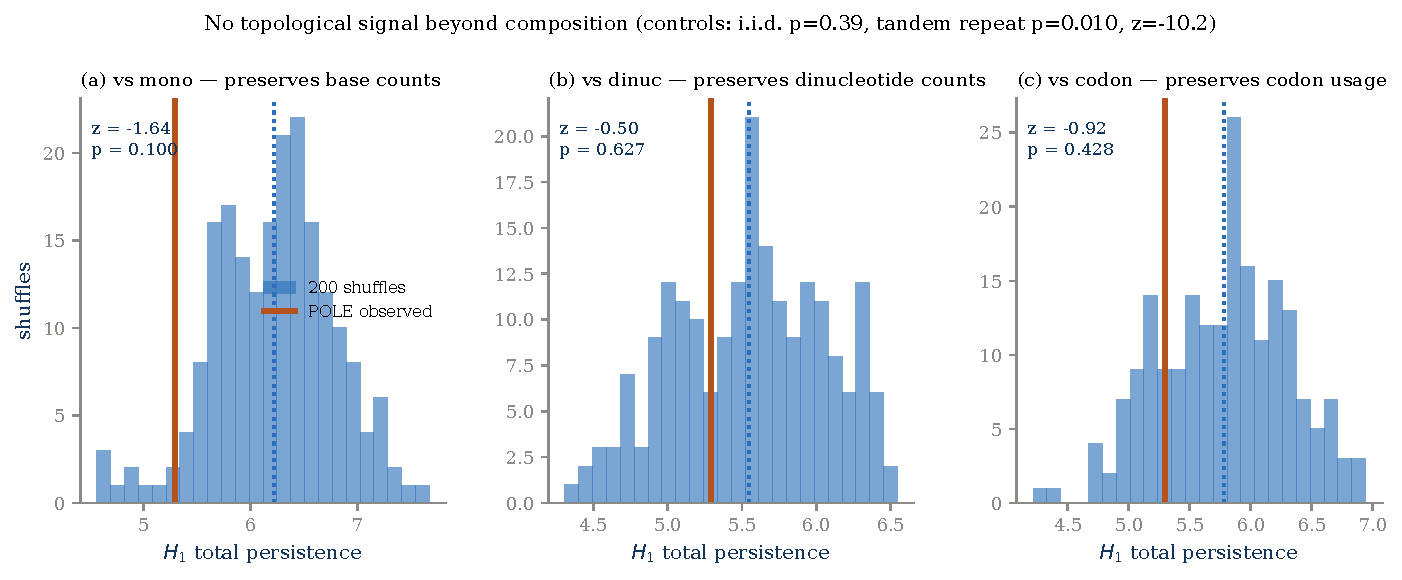
\includegraphics[width=\textwidth]{fig11_tda_null.pdf}
  \caption{The shuffle null for the \texttt{POLE} coding sequence. Each
  histogram is $200$ actual shuffle draws --- not a Gaussian fitted to two
  moments --- with the observed value in orange. The observed total persistence
  sits inside every null. Against \textbf{mono} it is $1.6$ standard deviations
  \emph{below} the null mean, and that modest displacement is fully absorbed once
  dinucleotide composition is preserved. Generated by
  \file{scripts/textbook/make_figures.py}, section~11, from
  \file{data/tda_sequence_null.json}.}
  \label{fig:tdanull}
\end{figure}

\subsubsection*{The result, stated plainly}

None of the three coding sequences shows a signal: every $p$ exceeds $0.05$, and
the largest displacement anywhere in the table is $1.8$ standard deviations. In
particular the \texttt{POLE} coding sequence has \textbf{no detectable topological signal
beyond its base composition}. Section~\ref{sec:tda}'s caution was correct, and
it is now earned rather than asserted.

Two details are worth more than the headline.

First, the displacement is \emph{negative}: the real sequence has slightly
\emph{less} $H_1$ persistence than its shuffles. Had we gone looking for
``structure'' we would have been looking in the wrong direction. A one-sided test
chosen after seeing the data would have reported $p \approx 0.95$ and we might
have called that a clean null; the two-sided test reports $0.099$, which is the
honest number and is still not significant.

Second, the mono-to-dinuc comparison localises what little there is. The $z$ of
$-1.64$ against \textbf{mono} falls to $-0.50$ against \textbf{dinuc}, so
whatever weak tendency exists is a \emph{dinucleotide composition} effect, not
higher-order sequence structure. That is a more informative negative than a bare
``not significant'', and it is only available because the nulls were nested.

\subsection{The artefact this section made, and how it was caught}\label{sub:strideartefact}

The first run of the experiment above reported a different result, and the way it
was wrong is more instructive than the corrected numbers.

\texttt{POLD1} appeared to carry a strongly significant signal: against the
mononucleotide null, $z = -3.59$ at the attainable $p$ floor of $0.010$, and
against the dinucleotide null $z = -2.90$, $p = 0.020$. Taken at face value this
was a genuine cross-sequence finding --- topological structure in one replicative
polymerase gene and not another --- and it is the sort of result one is tempted
to write up.

It was an artefact of our own sampling, and this book had already warned about
it. Worked Example~8.1 says, in those words, that a subsampling stride sharing a
factor with the reading frame over-samples one codon position, and that a stride
of $6$ or $9$ ``would have introduced a frame bias invisible in the final
diagram''. \texttt{POLD1}'s coding sequence is $3324$~nt, the subsample takes
$500$ points, and $3324 / 500$ rounds down to a stride of exactly $6$.

\begin{remark}[Why a frame-biased stride manufactures a signal]
The mechanism is worth following, because it explains both the false positive and
the clue that exposed it.

A stride of $6$ on a coding sequence visits only codon position~$1$, over and
over. Codon position~$1$ has its own base composition, markedly different from
the gene's overall composition. So the \emph{observed} cloud is built from a
compositionally skewed subsequence --- while the \textbf{mono} and \textbf{dinuc}
shuffles have no reading frame left to be biased by, and their clouds are built
from compositionally representative samples. Observed and null are then not
comparable, and the difference shows up as a displacement in total persistence.

Now the clue. The \textbf{codon} null permutes whole codons, so it
\emph{preserves} the reading frame --- and therefore suffers the identical
sampling bias. Against that null the bias cancels on both sides, and sure enough
\texttt{POLD1} gave $z = -0.44$, $p = 0.607$: no signal at all.

A finding that survives two nulls and vanishes against the third, where the
third is the only one preserving the frame, is not a finding about biology. It is
a signature, and reading it correctly requires having designed the nulls to be
nested in the first place.
\end{remark}

The fix is one line --- the stride is now chosen coprime with $3$, giving $13$
for \texttt{POLE}, $5$ for \texttt{POLD1} and $8$ for \texttt{MSH6} --- and it is
asserted in the script and in \file{tests/test_tda_null_and_orthologue.py}, so a
future change of point count cannot silently reintroduce it. Re-running is a
controlled comparison, because only \texttt{POLD1}'s stride changes: \texttt{POLE}
and \texttt{MSH6} were already coprime, so their numbers and the controls' must
come out identical, and they do. \texttt{POLD1}'s apparent signal does not
survive:

\medskip
\noindent
\texttt{POLD1}, $z$ of the $H_1$ total persistence against each null, before and
after the stride was made frame-safe:

\medskip
\begin{tabular}{@{}l r r r l@{}}
\toprule
\textbf{null} & \textbf{stride 6} & \textbf{stride 5} & \textbf{$p$} & \textbf{reading} \\
\midrule
mono  & $-3.59$ & $-0.83$ & $0.408$ & signal gone \\
dinuc & $-2.90$ & $+0.26$ & $0.945$ & signal gone \\
codon & $-0.44$ & $+0.26$ & $0.856$ & no signal either way \\
\bottomrule
\end{tabular}

\medskip
\noindent
The observed statistic itself moves, from $3.577$ to $5.007$, which is the direct
evidence that the biased stride was sampling a compositionally \emph{different}
subsequence and not merely a smaller one. Note also that the \textbf{codon} row's
$z$ changes, from $-0.44$ to $+0.26$: the prediction was never that this number
would stay fixed, but that it would show no signal in \emph{either} run, because
there the bias afflicts observed and null alike. It is the only row of which that
was true beforehand, and that is exactly why the artefact was visible.

\medskip
Three things are worth taking from this.

\emph{The warning was already in the book and did not prevent the error.} Knowing
about an artefact in the abstract is not the same as checking for it in your own
pipeline. The check is now code, not prose, which is the only form that
generalises.

\emph{The nested design did the work.} Had we run a single shuffle null --- the
usual practice --- the \texttt{POLD1} result would have been significant,
plausible and wrong, with nothing in the output to suggest otherwise. The third
null was not redundancy; it was the diagnostic.

\emph{The temptation ran the right way for once.} A spurious positive is easier
to publish than the negative result it displaced, and the only reason it was
examined at all is that it was surprising. That is a thin safeguard, and it is
why the stride is now asserted rather than inspected.

\begin{ledger}[Controls, because a null result is only as good as its power]
A null test that cannot come out positive is worthless, so both directions were
checked and both are asserted in code --- the script exits non-zero and writes
nothing if either fails.

\textbf{Negative control:} an i.i.d.\ sequence drawn from the real base
frequencies, which has no structure above composition by construction. Against
\textbf{mono} it gives $p = 0.388$, $z = +0.90$. Not flagged, as required: the
test does not manufacture signal.

\textbf{Positive control:} a tandem repeat of a single motif, composition-matched
to the real sequence so that only its \emph{order} differs. Against \textbf{mono}
it gives $p = 0.010$ --- the attainable floor --- at $z = -10.17$. Flagged
overwhelmingly, as required: the test has power to detect order.

So the negative result above is informative. A test that flagged a tandem repeat
at $z = -10$ and the real sequence at $z = -1.6$ is telling us something about
the sequence, not about its own insensitivity.
\end{ledger}

\subsection{Is yeast \texttt{P301} really human \texttt{P286}?}\label{sub:ortho}

The refutation of Section~\ref{sec:refutation} runs entirely through a yeast
allele. If \texttt{pol2-P301R} is not the structural analogue of human
\texttt{P286R}, the chain breaks at its first link --- and the book assumed the
correspondence without checking it.

\begin{numerics}[11.2]
\file{scripts/textbook/verify_yeast_human_correspondence.py}. Full-length global
alignment (Gotoh, affine gaps) of human \texttt{POLE} (UniProt \texttt{Q07864},
$2286$~aa) against \emph{S.~cerevisiae} \texttt{POL2} (\texttt{P21951},
$2222$~aa), both retrieved live with URLs and a UTC timestamp.

We have no verified substitution matrix on this host, and transcribing one from
memory is the kind of unchecked assertion this book argues against. So the
alignment is run under four explicit scoring schemes and gap costs, and the
result is reported only as \emph{invariant across them}. Human residue $286$
aligns to yeast residue $301$ in all four, at $43.1$--$44.8\%$ global identity.
\end{numerics}

The aligned neighbourhood is the real evidence, and it is worth printing:

\begin{center}
\begin{tabular}{@{}l l@{}}
human \texttt{POLE} $279$--$293$  & \texttt{T K L P L K F \textbf{P} D A E T D Q I} \\
yeast \texttt{POL2}\ $294$--$308$ & \texttt{T K P P L K F \textbf{P} D S A V D Q I} \\
\end{tabular}
\end{center}

\noindent
Eleven of fifteen positions are identical, and the substituted residue sits
inside an exactly conserved \texttt{F-P-D} tripeptide: human
$\texttt{F}285\,\texttt{P}286\,\texttt{D}287$ against yeast
$\texttt{F}300\,\texttt{P}301\,\texttt{D}302$. This is the ExoI motif, whose
aspartate is one of the two catalytic carboxylates that \texttt{pol2-4} replaces
with alanine.

\begin{figure}[htbp]
  \centering
  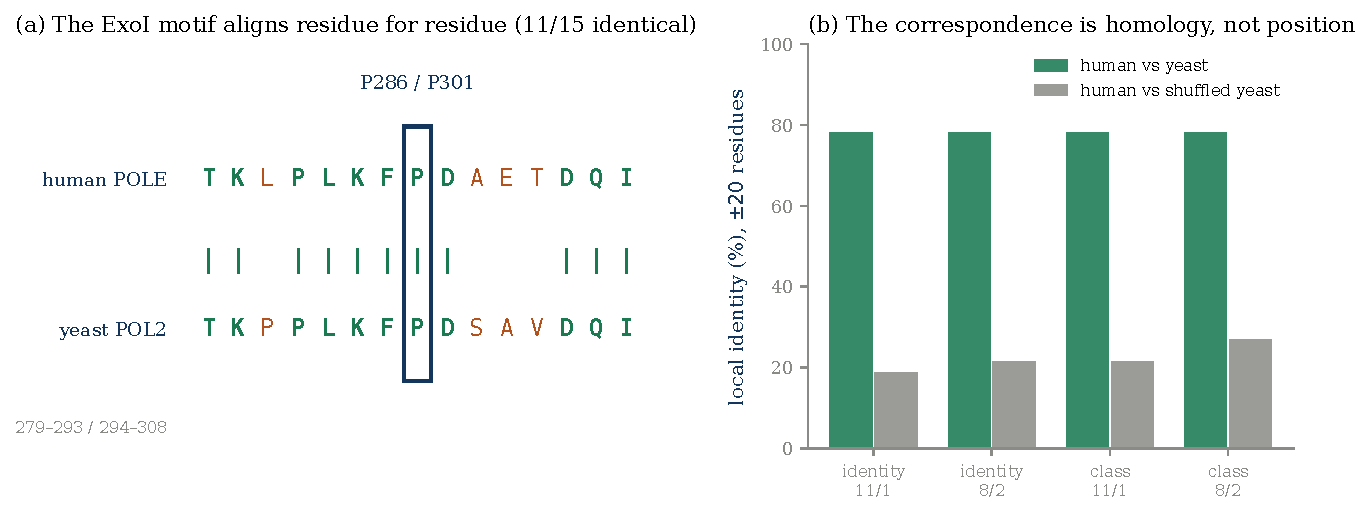
\includegraphics[width=\textwidth]{fig12_orthologue_alignment.pdf}
  \caption{(a) The aligned ExoI neighbourhood, residue by residue; green where
  identical. The boxed column is the substituted proline. (b) Local identity in
  a $\pm20$-residue window about the site, for the real pair against a
  composition-matched shuffle of the yeast sequence, under each scoring scheme.
  The real pair holds at $78.0\%$ throughout; the shuffle reaches at most
  $26.8\%$.}
  \label{fig:ortho}
\end{figure}

\begin{remark}[Which statistic actually carries the evidence]\label{rem:diagonal}
Here the verification taught us something we would have got wrong.

The obvious thing to report is ``human $286$ aligns to yeast $301$''. But that
claim is weaker than it looks, and the negative control shows why: aligning
human \texttt{POLE} against a \emph{shuffled} yeast sequence maps residue $286$
to residue $302$ --- one position away from the right answer. A global alignment
of two sequences of similar length follows the diagonal whatever the sequences
say, so positional agreement is largely a fact about the two lengths.

The statistic with no such prior is \emph{local conservation}. Around the site
the real pair holds $78.0\%$ identity against the shuffle's $26.8\%$, a factor of
$2.9$, under every scheme. That is the number the script gates on, and it is the
number a reader should be given.

The general lesson is the one from Section~\ref{sec:proof-and-cell} in a new
costume: ask what the control could have produced. A control that returns $302$
when the answer is $301$ has not validated anything, and quoting the position as
the result would have hidden that.
\end{remark}

So the correspondence holds. Note exactly what has been established: that the
two residues occupy the same position in a conserved motif. That is a claim about
sequence, and it is what the book needed. It is \emph{not} a claim that the two
enzymes respond identically to the substitution, which no alignment can settle.

\subsection{What if the stages interact?}\label{sub:interact}

Section~\ref{sec:nogo}'s ledger named one escape route from the no-go theorem,
and named it honestly: Assumption~\ref{model:class} requires stages to compose
multiplicatively and independently, and a model in which they \emph{interact} is
not covered. A reader could reasonably have replied: ``then the refutation only
kills the independent case, and you have not told me how much interaction it
would take to survive.''

That is a fair objection, and it has a number for an answer.

\begin{model}[Interacting stages]\label{model:interact}
Carry an explicit interaction factor $\Lambda \ge 0$:
\begin{equation}\label{eq:interact}
  \errate_\Lambda(\stages) \;=\; \inserr \Big(\prod_{i \in \stages} \escape_i\Big)\,\Lambda .
\end{equation}
$\Lambda = 1$ is exactly the independent class of Section~\ref{sec:nogo};
$\Lambda > 1$ says that losing stages is worse than multiplicativity predicts,
which is what ``the stages interact'' means quantitatively.
\end{model}

\begin{theorem}[The interacting ceiling, PSR$_2$I]\label{thm:psr2i}
Under the hypotheses of Assumption~\ref{model:class} together with
\eqref{eq:interact} and $\Lambda \ge 0$,
$\;\errate_\Lambda(\stages) \le \inserr\Lambda$ for every $\stages$.
\end{theorem}

\begin{proof}
The product lies in $[0,1]$, so $\inserr\prod \escape_i \le \inserr$; multiplying
by $\Lambda \ge 0$ preserves the inequality.
\end{proof}

\begin{theorem}[The price of the rescue, PSR$_3$I]\label{thm:psr3i}
If a variant keeping stages $\kept$ is measured at $\rho$ times the
exonuclease-null error, with $\inserr > 0$, then $\rho \le \Lambda$.
\end{theorem}

\begin{proof}
By Theorem~\ref{thm:psr2i} the observed rate $\rho\inserr$ is at most
$\inserr\Lambda$. Divide by $\inserr > 0$.
\end{proof}

\begin{figure}[htbp]
  \centering
  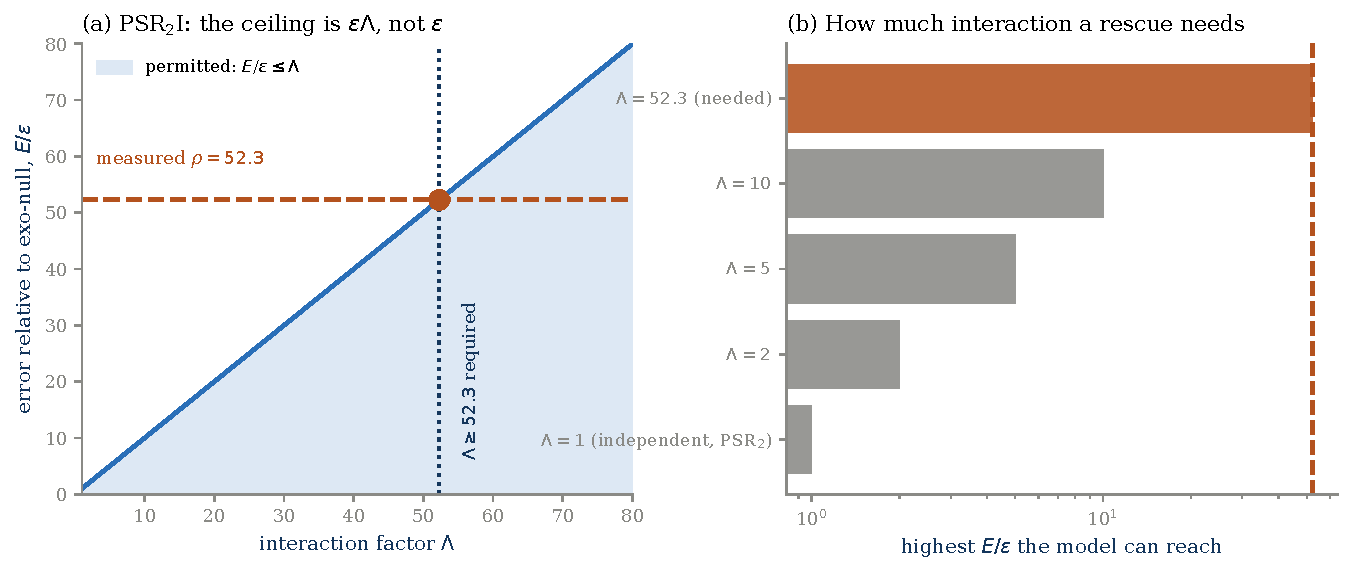
\includegraphics[width=\textwidth]{fig13_interaction_price.pdf}
  \caption{(a) The interacting ceiling. The permitted region is
  $\errate/\inserr \le \Lambda$; the measured $\rho = 52.3$ forces
  $\Lambda \ge 52.3$. (b) What each level of interaction can reach. The
  independent class of Section~\ref{sec:nogo} is the $\Lambda = 1$ bar, where the
  original ceiling returns.}
  \label{fig:interaction}
\end{figure}

\noindent
Put the measurement in. With $\rho = 2300/44 = 52.3$:

\begin{center}
\emph{A stage-removal account of \texttt{pol2-P301R} requires stages whose
interaction makes their loss at least $52$ times more damaging than independence
allows.}
\end{center}

This does not refute the interacting class, and it is important not to pretend
otherwise. What it does is convert a qualitative escape hatch into a
quantitative claim that an enzymologist can assess: is there any mechanism by
which three proofreading stages cooperate so strongly that removing them is
fifty-two-fold worse than their product? The question is now answerable, which it
was not before. Converting an unfalsifiable objection into a falsifiable one is
the whole service this book claims for formal methods, and here it is being
performed on an objection to the book's own argument.

\subsection{Formalisation}

\file{formal/ANSE/InteractingStagesAndTransport.lean}, $11$ of $11$ declarations
clean on the axiom gate.

\begin{lstlisting}
noncomputable def errorRateI {ι : Type*} (ε : ℝ) (q : ι → ℝ) (S : Finset ι)
    (Λ : ℝ) : ℝ := ε * (∏ i ∈ S, q i) * Λ

theorem PSR_3I_excess_forces_interaction {ι : Type*}
    (ε ρ Λ : ℝ) (hε : 0 < ε) (q : ι → ℝ)
    (h0 : ∀ i, 0 ≤ q i) (h1 : ∀ i, q i ≤ 1)
    (T : Finset ι) (hΛ : 0 ≤ Λ)
    (hobs : errorRateI ε q T Λ = ρ * ε) : ρ ≤ Λ
\end{lstlisting}

\noindent
The module also carries \lean{psr2I_recovers_psr2}, which shows the original
ceiling returns at $\Lambda = 1$ --- the control confirming that $\Lambda$ is
load-bearing and not decoration --- and
\lean{interaction_hypotheses_satisfiable}, a witness that the hypotheses of
Theorem~\ref{thm:psr3i} are jointly satisfiable with a nontrivial product and
$\rho > 1$. Without the witness the theorem could hold merely because nothing
meets its assumptions.

\subsubsection*{The transport problem, as a theorem}

Remark~\ref{rem:transport} argued that Section~\ref{sec:mmr}'s conclusion rests
on carrying an in vitro inequality into a cell. That was prose. The same module
makes it arithmetic. Writing production as
$\mathrm{prod}(e,s) = e\cdot s$, with $e$ the error rate per nucleotide and $s$
the nucleotides synthesised per replicated genome:

\begin{lstlisting}
theorem per_nucleotide_does_not_transport :
    ∃ eMut eNull sMut sNull : ℝ,
      0 ≤ eMut ∧ 0 ≤ eNull ∧ 0 ≤ sMut ∧ 0 ≤ sNull ∧
      eMut ≤ eNull ∧
      production eNull sNull < production eMut sMut

theorem transport_needs_synthesis_bound (eMut eNull sMut sNull : ℝ)
    (he0 : 0 ≤ eMut) (hs0 : 0 ≤ sMut)
    (he : eMut ≤ eNull) (hs : sMut ≤ sNull) :
    production eMut sMut ≤ production eNull sNull
\end{lstlisting}

The first is a counterexample, and the witness is the measured enzyme in
miniature: $e = 59$ against $155$, $s = 40$ against $4$. More accurate per
nucleotide, four times the delivered load. The second names the missing
hypothesis exactly --- $s_{\mathrm{mut}} \le s_{\mathrm{null}}$ --- and it is a
statement about how much of the genome each enzyme copies, which no experiment
in this book measures.

A caveat is now a theorem, which means it can no longer be forgotten.

\subsection{What the combination buys}\label{sub:combination}

This book has used machine-checked proof, exact and numerical computation, live
database retrieval, and computational topology on the same problem. It is worth
being precise about what each contributed, because the honest accounting is
uneven and the uneven parts are the instructive ones.

\begin{itemize}[leftmargin=*,itemsep=3pt]
  \item \textbf{Proof contributed the refutation.} PSR$_2$ has no free
        parameters, so one ratio killed a mechanism class. That is the single
        most consequential step in the book, and it was available only because
        the hypothesis had been stated precisely enough to be refuted.
  \item \textbf{Proof also contributed the limits of the refutation.}
        Theorem~\ref{thm:psr3i} prices the escape route;
        \lean{per_nucleotide_does_not_transport} exhibits the gap in the
        replacement mechanism. Formalisation was at least as useful pointed at
        our own conclusions as at the one we overturned.
  \item \textbf{Numerics contributed a correction.} The Luria--Delbrück
        simulation of Section~\ref{sec:accumulation} did not confirm the closed
        form; it exposed that the variance is not estimable at any feasible
        number of cultures (\S\ref{sub:trap}). The computation was useful
        precisely by disagreeing.
  \item \textbf{Retrieval contributed two corrections.} The live scripts caught
        a wrong assumption about ClinVar's categories partitioning, and a wrong
        source for domain boundaries. Both were our errors, found because the
        data were fetched and checked rather than quoted.
  \item \textbf{Topology contributed a negative result.} \S\ref{sub:tdanull} is
        the honest answer to the question Section~\ref{sec:tda} raised, and the
        answer is no. This is the most conspicuous case of a method producing a
        beautiful picture and no biological knowledge, and it is in the book for
        that reason.
\end{itemize}

\begin{remark}[The absent layer line, again]\label{rem:franklin-again}
It is worth noticing what kind of evidence this section's central result is,
because the book is dedicated to someone whose decisive evidence was of the same
kind.

Photo~51's contribution was in part an \emph{absence}: the fourth layer line is
missing, and \S\ref{sub:photo51} shows that a two-strand helix offset by
$\delta = 3/8$ requires it to be missing. An absence is only evidence if the
method could have shown the thing. Franklin's plate could --- the neighbouring
layer lines are plainly there, which is precisely why the gap at $n = 4$ means
something. Had the exposure been too short to show any layer lines, their absence
would have meant nothing at all.

\S\ref{sub:tdanull} is an absence of exactly this structure. The claim is that
\texttt{POLE} shows no topological signal beyond composition, and that claim is
worth something only because the same test flagged a composition-matched tandem
repeat at $z = -10.2$. The positive control plays the role the visible layer
lines play on the plate: it establishes that the method can see.

This is, we think, the most useful single habit in the book. A negative result
and an unperformed experiment produce the same number of significant findings,
and are told apart only by the control. State it, or the absence is just silence.
\end{remark}

\begin{remark}[On the temptation that topology presents]
It would have been easy to publish Figure~\ref{fig:tda} with a sentence about
``the intrinsic topological signature of the \texttt{POLE} locus'' and no null.
The picture is striking, the method is fashionable, and almost no reader checks.
Running the null cost an afternoon and produced a result that is harder to
publish and more worth having.

We single this out because the incentive gradient runs the wrong way, and a
student should know that in advance. The methods in this book that most readily
produce impressive output --- high-dimensional embeddings, persistence diagrams,
and anything with a $3$D rendering --- are exactly the ones whose nulls are most
often omitted.
\end{remark}

\subsection{The human stakes, stated carefully}

The user of a textbook is entitled to ask what any of this is for, and the
answer should not be inflated.

Nothing in this book has treated a patient. The refutation of
Section~\ref{sec:refutation} does not change the management of a
\texttt{POLE}-mutant tumour, and Section~\ref{sec:clinic} explains why the
clinical decision rule was never load-bearing on the mechanism. The topology is a
negative result. The alignment confirms something the field already assumed.

What has been produced is narrower and real: one retracted mechanism, a sharper
question about mismatch repair, a priced escape route, a named missing
measurement, and a worked demonstration that each of these can be found by
reading one's own claims adversarially.

The argument for the value of that is an argument about aggregate harm. Wrong
mechanisms in the biomedical literature are not harmless. They direct grant
money, select which experiments get done, and shape which variants a clinician
treats as explained. They persist because mechanisms are usually stated loosely
enough to accommodate contrary data --- and the remedy is not better intentions
but statements sharp enough to fail. Every retraction in this book was possible
only because something had been written down precisely.

The care for the people downstream, then, looks like this in practice: state the
mechanism as a model class, prove what the class entails without fitting,
compare against a directly measured reference, run the control that could
embarrass you, and publish the refutation when it comes --- including when it is
your own. It requires no new technology. It requires being willing to be wrong in
public, on the record, with the date attached.

That is the whole method. A student who takes nothing else from this book should
take the habit of asking, of every claim including their own: \emph{what would
have had to happen for this to come out differently?} If the answer is nothing,
there is no evidence there, however good the figure looks.

\begin{worked}[11.1: reading a negative result correctly]
\textbf{Problem.} A colleague summarises \S\ref{sub:tdanull} as ``persistent
homology does not work on DNA sequence''. Is that what was shown?

\textbf{Solution.} No, and the overstatement runs in the opposite direction to
the usual one. Three narrower things were shown.

\emph{(i)} For \emph{this} statistic ($H_1$ total persistence), \emph{this}
embedding (3D chaos game), \emph{this} sequence (the \texttt{POLE} CDS) and
\emph{these} nulls, no signal exceeds composition. \emph{(ii)} The test had power
to detect gross order structure, since a composition-matched tandem repeat was
flagged at $z = -10.2$. \emph{(iii)} The weak residual against \textbf{mono}
disappears against \textbf{dinuc}, localising it to dinucleotide composition.

What was not shown: that no statistic, embedding or sequence class would give a
signal. A negative result bounds the methods actually run. Generalising it to
``TDA does not work'' is the same category error as generalising \texttt{V411L}'s
quiet behaviour in one background to ``functionally neutral''
(Worked Example~7.1) --- an absence of effect in one setting reported as an
absence in all.
\end{worked}

\begin{worked}[11.2: how much interaction is 52-fold?]
\textbf{Problem.} Theorem~\ref{thm:psr3i} requires $\Lambda \ge 52.3$. Express
this as a statement about per-stage factors, and judge its plausibility.

\textbf{Solution.} With three stages at $\escape_i = \gamma$ the independent
model gives $\errate = \inserr\gamma^3$. The interacting model with the same
$\gamma$ reaches $\inserr\gamma^3\Lambda$, so $\Lambda = 52.3$ is equivalent to
an \emph{effective} per-stage factor $\gamma' = \gamma\,\Lambda^{1/3} = 3.74\gamma$:
each stage would have to be nearly four times leakier in the mutant than its own
measured escape probability, purely by virtue of the others being absent.

Judging plausibility is not a mathematical question, and the theorem does not
pretend to settle it. But it has become the right question, and it is addressed
to enzymology rather than to algebra. Note also that
Section~\ref{sec:refutation}'s in vitro measurement constrains it independently:
the purified enzyme is \emph{more} accurate than exonuclease-null, which is hard
to reconcile with stages that have become four-fold leakier.
\end{worked}

\begin{exercise}
The nulls of Assumption~\ref{model:tdanull} are nested: each preserves what the
previous one preserved and more. Explain why nesting makes a negative result more
informative than three unrelated nulls would, and state what a fourth null
preserving trinucleotide counts would add.
\end{exercise}

\begin{exercise}
\S\ref{sub:tdanull} reports a two-sided $p$ of $0.099$ against \textbf{mono},
and notes that a one-sided test chosen after seeing the data would have reported
$0.95$. Explain why choosing the direction after seeing the data invalidates the
$p$-value, and how a pre-registered direction would have been chosen here.
\end{exercise}

\begin{exercise}
Remark~\ref{rem:diagonal} argues that positional agreement in a global alignment
carries a diagonal prior. Design a control that removes it --- for instance by
shuffling only within the domain, or by aligning against a reversed sequence ---
and say what each choice preserves and destroys.
\end{exercise}

\begin{exercise}
Prove Theorem~\ref{thm:psr2i} directly from Theorem~\ref{thm:psr2} without
re-deriving the product bound. Then explain why the Lean module proves it
independently rather than as a corollary.
\end{exercise}

\begin{exercise}[(harder)]
\lean{per_nucleotide_does_not_transport} exhibits $e = 59$ against $155$ and
$s = 40$ against $4$. The error rates are the measured ones; the synthesis
figures are invented to make the point. Find the actual constraint: given the
measured $e$ values, what is the smallest ratio $s_{\mathrm{mut}}/s_{\mathrm{null}}$
that would invert the delivered load? Then say what experiment would measure
that ratio.
\end{exercise}

\begin{exercise}[(harder)]
\S\ref{sub:combination} claims the methods contributed unevenly, with topology
contributing a negative result and proof contributing the refutation. Construct
the opposite case: describe a biological question on which persistent homology
would carry the argument and a no-go theorem would be useless. What structural
feature of the question decides which method applies?
\end{exercise}

\begin{ledger}
\textbf{Measured:} $H_1$ total persistence of the \texttt{POLE}, \texttt{POLD1}
and \texttt{MSH6} coding sequences against $200$ shuffles from each of three
nulls, with both controls passing
(\file{data/tda_sequence_null.json}). Full-length alignment of
\texttt{Q07864} against \texttt{P21951}, retrieved live, under four scoring
schemes with both controls passing
(\file{data/yeast_human_correspondence.json}). \\
\textbf{Assumed:} that $H_1$ total persistence is a reasonable summary of the
persistence diagram --- a different statistic could behave differently, and this
one was fixed before the nulls were run. That the four scoring schemes of
\S\ref{sub:ortho} span enough of the space for ``invariant'' to mean something;
they are not a substitute for a validated substitution matrix. That
\eqref{eq:interact} is a fair way to parameterise interaction, which it is for a
single lumped factor and is not if interactions are stage-specific. \\
\textbf{Proved:} Theorems~\ref{thm:psr2i} and~\ref{thm:psr3i}
(\lean{PSR_2I_interacting_ceiling}, \lean{PSR_3I_excess_forces_interaction}),
with the control \lean{psr2I_recovers_psr2} and a non-vacuity witness; the
transport counterexample \lean{per_nucleotide_does_not_transport} and its
repair \lean{transport_needs_synthesis_bound}. Gate: $11$ of $11$ clean, no
\lean{sorryAx}. \\
\textbf{Open:} the trinucleotide null of Exercise~11.1 is not run. The
synthesis ratio of Exercise~11.5 is not measured and is the single most useful
missing experiment in this book. Whether $\Lambda \ge 52$ is achievable by any
real cooperative mechanism is a question for enzymology and is not addressed
here. And the alignment establishes positional correspondence only; that the two
enzymes respond equivalently to the substitution remains assumed. \\
\textbf{Discharged by this section:} the \textbf{Open} lines of
Sections~\ref{sec:nogo}, \ref{sec:mmr}, \ref{sec:variants} and
\ref{sec:tda} concerning interaction, transport, the yeast--human
correspondence and the shuffle null respectively. \\
\textbf{Where the remaining open items go:}
Appendix~\ref{app:directions} collects every \textbf{Open} line in this book
into a ranked work programme, with a first step and a falsification criterion
for each. The single measurement we would most like someone to make is the
synthesis ratio of Exercise~11.5, and it is D1 there.
\end{ledger}

% =============================================================================
% Section 12 — Reticulate evolution, and a null that is a theorem
% =============================================================================
\section{Reticulate Evolution: When the Null Can Be a Theorem}\label{sec:reticulata}

\begin{objectives}
\begin{itemize}[leftmargin=*,itemsep=1pt,topsep=1pt]
  \item State the ultrametric and four-point conditions, and say which biological assumption each one encodes.
  \item Prove that every symmetric ultrametric satisfies the four-point condition, and read off what a quartet violation refutes.
  \item Explain why a violation of ultrametricity is \emph{not} evidence of recombination, using the relaxed-clock control that refuted that reading.
  \item Compute a four-point verdict by hand from six integer counts under complete deletion.
  \item Say what a machine-checked certificate does and does not vouch for once the data has passed through an aligner.
\end{itemize}
\end{objectives}

\subsection{What Section 8 got wrong, and the shape of the repair}

Section~\ref{sec:tda} embedded one DNA sequence by the chaos game and measured
the topology of the resulting point cloud. Section~11 ran the null that section
had declined to run, and the answer was negative. It is worth being precise
about why, because the diagnosis determines the repair.

The chaos game contracts \emph{any} sequence onto a self-similar attractor. The
holes being measured were therefore the attractor's, not the sequence's. With no
mathematical null available, the test had to be calibrated against shuffles,
which bought a $p$-value floor, a frame-sampling artefact (\S11.3), and a
statistic with no proved meaning.

The repair is not a better statistic on the same object. It is a different
object. Following Chan, Carlsson and Rabadan, compute topology on a
\emph{population} of sequences under a genetic distance. There, a
one-dimensional cycle has an interpretation: it indicates non-tree-like,
\emph{reticulate} evolution --- recombination in a virus, reassortment between
influenza segments, horizontal transfer between bacteria. And --- this is the
part that is new in these pages --- the null becomes a theorem instead of an
ensemble.

\subsection{Two nulls, and the fact that they nest}

Write $d(x,y)$ for the $p$-distance between two aligned sequences: the number of
columns at which they differ, over the number of columns at which both are
comparable.

\begin{definition}[Ultrametric]\label{def:ultrametric}
A symmetric $d$ is \emph{ultrametric} when for all $x,y,z$
\begin{equation}\label{eq:ultrametric}
  d(x,z) \;\le\; \max\!\left(d(x,y),\, d(y,z)\right).
\end{equation}
\end{definition}

\begin{model}[What \eqref{eq:ultrametric} assumes]\label{mod:clock}
Expected $p$-distances are ultrametric exactly when descent is \textbf{clonal}
--- the genealogy is a tree --- \textbf{and} the molecular clock is
\textbf{strict}, so that every lineage accumulates substitutions at the same
rate. Two assumptions, one inequality. Remember that; \S\ref{sub:relaxed}
turns on it.
\end{model}

The consequence that makes \eqref{eq:ultrametric} useful is immediate and worth
seeing. If $d$ is ultrametric then the relation $d(\cdot,\cdot)\le\epsilon$ is
transitive, so every connected component of the Vietoris--Rips complex at scale
$\epsilon$ is a clique --- a filled simplex. An \emph{unfilled} cycle therefore
cannot occur at any scale. Three sequences with
\begin{equation}\label{eq:certificate}
  \max\!\left(d(x,y),\, d(y,z)\right) \;<\; d(x,z)
\end{equation}
are not a surprise relative to shuffles. They are a \textbf{certificate} that
the data is not ultrametric. Nothing is being calibrated; a universally
quantified statement is being contradicted by a witness.

\begin{definition}[Four-point condition]\label{def:fourpoint}
A symmetric $d$ satisfies the \emph{four-point condition} when for all
$a,b,c,e$
\begin{equation}\label{eq:fourpoint}
  d(a,b) + d(c,e) \;\le\;
  \max\!\big(d(a,c)+d(b,e),\; d(a,e)+d(b,c)\big).
\end{equation}
\end{definition}

A quadruple admits three ways of pairing its members. Condition
\eqref{eq:fourpoint} says no pairing's distance sum strictly exceeds both
others. That is a statement about \emph{tree structure} with no constraint on
rates at all: branch lengths are free. By Buneman's theorem a metric satisfying
\eqref{eq:fourpoint} on every quadruple is realised by a weighted tree. We cite
that converse; we do not prove it, and the book says so rather than implying
otherwise.

Now the result that organises everything else.

\begin{theorem}[The nulls nest]\label{thm:nesting}
Every symmetric ultrametric satisfies the four-point condition.
\end{theorem}

\begin{proof}
Fix $a,b,c,e$. Applying \eqref{eq:ultrametric} four times, with symmetry to put
each application in the right order,
\[
  d(a,b) \le \max\!\big(d(a,c),d(b,c)\big), \qquad
  d(a,b) \le \max\!\big(d(a,e),d(b,e)\big),
\]
\[
  d(c,e) \le \max\!\big(d(a,c),d(a,e)\big), \qquad
  d(c,e) \le \max\!\big(d(b,c),d(b,e)\big).
\]
Each bound is a disjunction, so there are $2^4$ cases. In each, split further on
the order of the four quantities $d(a,c), d(a,e), d(b,c), d(b,e)$ that appear.
Every branch gives $d(a,b)+d(c,e)$ bounded by one of the two right-hand sums of
\eqref{eq:fourpoint} by a linear arithmetic step. The case analysis is tedious
by hand and is exactly the sort of thing a kernel should do: see
Listing~\ref{lst:nesting}.
\end{proof}

\begin{corollary}[What a quartet violation buys]\label{cor:quartet}
If $d$ is symmetric and fails \eqref{eq:fourpoint}, then $d$ is not ultrametric
either.
\end{corollary}

So the two nulls are nested, and Corollary~\ref{cor:quartet} says a quartet
violation refutes \emph{strictly more} than a triple violation does. This is the
licence --- a theorem, not a convention --- for the reading that organises
\S\ref{sub:relaxed}: large triple margins together with floor-level quartet
margins indicate rate variation on a tree, because that is the region the
nesting leaves available.

\subsection{Formalisation}

\begin{lstlisting}[caption={The nesting theorem and its corollary, from \texttt{formal/ANSE/GeneticaReticulataTree.lean}. The \texttt{rcases} chain is the $2^4$ case split of the proof above, with four more splits on the order of the bounding quantities; \texttt{linarith} closes each branch.},label={lst:nesting}]
def IsFourPoint (d : α → α → ℚ) : Prop :=
  ∀ a b c e, d a b + d c e ≤ max (d a c + d b e) (d a e + d b c)

theorem fourPoint_of_ultrametric {d : α → α → ℚ}
    (hsym : ∀ x y, d x y = d y x) (hu : IsUltrametric d) : IsFourPoint d := by
  intro a b c e
  have h1 : d a b ≤ max (d a c) (d b c) := by
    have := hu a c b; rwa [hsym c b] at this
  have h2 : d a b ≤ max (d a e) (d b e) := by
    have := hu a e b; rwa [hsym e b] at this
  have h3 : d c e ≤ max (d a c) (d a e) := by
    have := hu c a e; rwa [hsym c a] at this
  have h4 : d c e ≤ max (d b c) (d b e) := by
    have := hu c b e; rwa [hsym c b] at this
  rw [le_max_iff] at h1 h2 h3 h4
  rw [le_max_iff]
  rcases h1 with h1 | h1 <;> rcases h2 with h2 | h2 <;>
    rcases h3 with h3 | h3 <;> rcases h4 with h4 | h4 <;>
    rcases le_total (d a c) (d a e) with k2 | k2 <;>
    rcases le_total (d a c) (d b c) with k3 | k3 <;>
    rcases le_total (d b e) (d a e) with k4 | k4 <;>
    rcases le_total (d b e) (d b c) with k5 | k5 <;>
    first | (left; linarith) | (right; linarith)

theorem quartet_violation_refutes_ultrametric {d : α → α → ℚ}
    (hsym : ∀ x y, d x y = d y x) (h : ¬ IsFourPoint d) : ¬ IsUltrametric d :=
  fun hu => h (fourPoint_of_ultrametric hsym hu)
\end{lstlisting}

The module carries sixteen theorems through the axiom gate of
\S\ref{sec:proof-and-cell}: zero \texttt{sorry}, and no axioms beyond
$\{\texttt{propext}, \texttt{Classical.choice}, \texttt{Quot.sound}\}$. It also
carries the controls, which matter more than the theorems. One witness shows the
violating configuration is realisable, so the statement is not vacuous; one
control shows a tree quadruple admits no certificate; one shows a forged
certificate is impossible; and one --- \S\ref{sub:deletion} explains why ---
exhibits three sequences on which pairwise deletion grants a certificate that
complete deletion denies.

\subsection{The obvious statistic is the wrong one}\label{sub:relaxed}

Condition \eqref{eq:certificate} is cheap: it needs three sequences, not four.
The first version of this work therefore reported it, and reported a clean
separation between a simulated clonal population and a simulated recombinant.
That separation was real and the inference drawn from it was wrong, for the
reason Modelling Assumption~\ref{mod:clock} warns about: ultrametricity bundles
two assumptions, and violating it tells you only that \emph{one} of them failed.

The decisive control is a \textbf{divergence-matched relaxed clock}: clonal
descent on a tree, no reticulation whatever, but with each lineage's substitution
rate multiplied by a random factor. Matching matters. For a multiplier
$e^{s u}$ with $u$ uniform on $[-1,1]$ one has
$\mathbb{E}[e^{su}] = \sinh(s)/s > 1$, so an unnormalised relaxed clock is also
a \emph{faster} clock, and a violation could then be blamed on saturation rather
than on rate variation. Dividing by that mean leaves the expected divergence
equal to the strict-clock case while the realised rates vary widely.

\begin{numerics}[12.1: the control that refutes the triple statistic]
Thirty-two leaves, $4000$ nt, three seeds, exhaustive over all $35\,960$
quadruples. Margins are exact rationals with denominator $4000$; the table gives
numerators, seed by seed.

\begin{center}\small
\begin{tabular}{@{}lcc@{}}
\toprule
simulated population & triple margin & quartet margin \\
\midrule
clonal, strict clock (null)            & $24,\ 30,\ 29$     & $10,\ 9,\ 10$ \\
clonal, \textbf{relaxed} clock (null)  & $155,\ 157,\ 99$   & $11,\ 18,\ 8$ \\
one recombinant                        & $79,\ 77,\ 75$     & $79,\ 70,\ 69$ \\
two reciprocal mosaics                 & $79,\ 77,\ 75$     & $158,\ 154,\ 126$ \\
\bottomrule
\end{tabular}
\end{center}

Read the second and third rows together. The smallest triple margin produced by
a population with \emph{no reticulation in it at all} is $99/4000$; the largest
produced by a population with a real recombinant is $79/4000$. The ordering is
inverted, at every seed. The quartet column does not move: the relaxed clock
stays at the level of the strict clock, while the reciprocal-mosaic positive
control separates from it by a factor of $12.6$ at its weakest seed.

Adding taxa makes the triple statistic worse, as the mechanism predicts: the
statistic is a maximum over triples, so more leaves give more chances at an
extreme pair of rates.

Produced by \texttt{reticulation experiment}; results in
\texttt{data/reticulata\_phase2/experiment\_n32.json}.
\end{numerics}

\begin{remark}[The recommendation, and its licence]
Report the \textbf{quartet} statistic as primary. Keep the triple statistic ---
it is cheaper, and a triple violation with \emph{no} quartet violation is
informative in its own right, being the signature of rate variation on a tree
--- but a triple certificate alone is not evidence of reticulation. What makes
the second half of that sentence more than a hunch is
Theorem~\ref{thm:nesting}.
\end{remark}

\subsection{Missing data: complete deletion within the subset}\label{sub:deletion}

Real alignments have gaps. The usual convention, \emph{pairwise deletion},
computes each pair's distance over the columns comparable in that pair --- which
gives different pairs different denominators. That alone can break
\eqref{eq:ultrametric} on a genealogy that is exactly a clock tree, with no
reticulation present: an adversarial audit of the first version of this work
found a case and the Lean module now carries it as a control.

The fix is \emph{complete deletion within the subset}: count only the columns at
which \emph{every} member of the triple or quadruple carries a definite base.
All distances in a certificate then share one denominator, and the obligations
become comparisons between integers --- no cross-multiplication, a smaller
trust surface, and the repair, all at once.

\begin{numerics}[12.2: how large the confound is]
Gap-blocked but strictly clonal, strictly clock-like populations, sixteen taxa,
$4000$ nt, five seeds. Pairwise deletion calls $33$ to $52$ of the $560$ triples
violations that complete deletion within the triple denies --- six to nine per
cent --- at every seed. At thirty-two taxa, $286$ to $366$ of $4960$. With no
missing data the two policies agree on all $560$, as they must.

The cost is power: at a $25\%$ gap load roughly $1000$ to $1700$ of the $4000$
columns survive inside a triple.
\end{numerics}

\begin{remark}[Margins under the two policies are not comparable]
Complete deletion shrinks the denominator, so one differing site is worth more
and its margins come out \emph{larger}, although the policy is strictly more
conservative. A criterion comparing the two sets of margins was written into the
first run of this experiment and had to be withdrawn. Compare per-subset
\emph{verdicts}, not magnitudes. This failure mode --- comparing numbers whose
denominators, reference populations or sequence lengths differ --- is the single
most frequent error in this book's own history, and \S11.3 is another instance.
\end{remark}

\subsection{The aligner is part of the trust surface}\label{sub:aligner}

A certificate is machine-checked, so it is tempting to say the conclusion does
not depend on the pipeline. It is not true, and the precise statement is worth
having.

The kernel is handed the sequences and recomputes every count from them by
\texttt{rfl}. So a false inequality, a wrong count, a transposed pair or a
miscomputed margin is excluded. What remains trusted is that the embedded rows
are the data they are claimed to be --- and on real data those rows come out of
an \textbf{aligner}. If the alignment puts non-homologous residues in the same
column, the counts are computed faithfully from the wrong data and the kernel
accepts them.

That cannot be proved away, so it is measured. Simulate clonal, relaxed-clock
descent with deletion events in a fixed coordinate frame; the frame \emph{is}
the true alignment. Strip the gaps, hand the ragged sequences to the aligner,
realign, and compare per-quadruple verdicts. Any quadruple the inferred
alignment calls a four-point violation and the true alignment does not was
manufactured by the aligner, on a genealogy with no reticulation in it.

\begin{numerics}[12.3: the admissibility ladder]
Sixteen taxa, $4000$ nt, five seeds, $1820$ quadruples each, reference-anchored
affine-gap alignment. Raising the deletion load:

\begin{center}\small
\begin{tabular}{@{}cccrr@{}}
\toprule
mean deletion & inferred gap & worst column & quadruples & seeds with \\
length (nt) & fraction & recovery & manufactured & any \\
\midrule
 30 & $0.0000$ & $1.0000$ & $0$    & $0/5$ \\
 30 & $0.0040$ & $1.0000$ & $0$    & $0/5$ \\
 30 & $0.0055$ & $0.9988$ & $251$  & $2/5$ \\
 30 & $0.0149$ & $0.9928$ & $217$  & $3/5$ \\
 30 & $0.0237$ & $0.9753$ & $1537$ & $4/5$ \\
120 & $0.0132$ & $0.9990$ & $57$   & $2/5$ \\
120 & $0.0474$ & $0.8939$ & $2613$ & $5/5$ \\
120 & $0.0941$ & $0.8681$ & $4876$ & $5/5$ \\
\bottomrule
\end{tabular}
\end{center}

At the heaviest rung the aligner manufactures $4876$ of the $9100$ quadruple
verdicts. Alignment error is not a rounding error in this test; past a
threshold it \emph{is} the result.

The threshold is therefore read off the ladder rather than chosen: a gap
fraction of $0.0040$ and an insertion load of $8.1\times10^{-4}$ dropped
residues per aligned cell, the heaviest rung at which nothing was manufactured
at any seed. Both are rates, not counts, because an absolute insertion count is
not comparable between a $3$~kb and a $12$~kb genome.

Produced by \texttt{reticulation align-error}; results in
\texttt{data/reticulata\_phase3/align\_error.json}.
\end{numerics}

\begin{remark}[A tie-break that was nearly a result]
The control that the aligner is the identity on gapless input failed at one seed
of five on the first implementation, and the cause was not a bug in the dynamic
programme. With an affine gap of $-10$ to open and $-1$ per residue, three
consecutive mismatches score $3\times(-4) + 5 = -7$, and deleting one reference
residue, aligning the rest, and inserting one query residue scores
$-11 + 15 - 11 = -7$ as well. The identity was one of two optimal alignments and
the implementation returned the other. The repair was to \emph{state} the
preference --- substitution over gap pair --- and the lesson is that an aligner
has free parameters that no amount of downstream proof will constrain.
\end{remark}

\subsection{Real populations}\label{sub:realdata}

Five viral taxa were drawn from the \texttt{hiyata/Virus-Host-Genomes} corpus
($58\,046$ genomes with taxonomy) under filters fixed in advance: near-median
length, at most $0.1\%$ ambiguous residues, exact duplicates removed, sixteen
sequences per population, selected either in accession order or by greedy
$6$-mer diversity. Each taxon carries a \emph{literature} expectation, written
before any margin was computed, and the test is free to contradict it.

\begin{center}\small
\begin{tabular}{@{}llp{0.40\textwidth}@{}}
\toprule
taxon & expectation & why \\
\midrule
Hepatitis B virus & reticulate & inter-genotype recombinants are recognised taxonomic entities \\
Coxsackievirus A6 & reticulate & lineages are named by recombinant form \\
Lyssavirus rabies & tree-like & non-segmented negative-strand RNA; recombination reported only exceptionally \\
Papillomavirus 52 & tree-like & co-divergence with the host; within-type recombination considered rare \\
JC polyomavirus & tree-like & genotypes track human migration and are analysed as a tree \\
\bottomrule
\end{tabular}
\end{center}

Seven of the ten populations fail the admissibility gate of
Numerics~12.3 and are reported BLOCKED with their counts rather than
interpreted. That is expensive --- some of the blocked numbers look interesting
--- and it is the point: the alternative is a claim about a virus that is really
a claim about a dynamic-programming tie-break. The three that pass are each run
twice, on two different alignment references, and each margin is compared
against a floor from a simulated clonal relaxed-clock tree at \emph{matched}
alignment width, \emph{matched} mean $p$-distance and \emph{matched} gap load.

\begin{numerics}[12.4: what the three admissible populations say]
\begin{center}\footnotesize
\begin{tabular}{@{}llrrl@{}}
\toprule
population & expected & margin & floor & verdict \\
\midrule
Hepatitis B, accession & reticulate & $9/3182$ & $2/3182$ & above $2\times$ \\
Coxsackievirus A6, spread & reticulate & $329/7312$ & $268/7390$ & above $1\times$ \\
JC polyomavirus, accession & tree-like & $4/5108$ & $24/5121$ & below \\
\bottomrule
\end{tabular}
\end{center}

Three populations, three agreements with the prior, and the two alignment
references agree on the verdict in all three. Both populations that clear their
floor carry a Lean file embedding the four aligned rows, so the kernel
recomputes the six pair counts and the common column count itself: accepted at
$3182$ columns in $67.8$~s and at $7434$ columns in $130.5$~s, with both
corrupted twins rejected. These are the first findings in this programme on data
that was not simulated which a reader can re-verify without running any of our
code.

Three populations is not a validation. It is the first time this test has been
run on data that was not simulated, with the aligner's contribution bounded by a
measurement rather than assumed away.
\end{numerics}

\subsection{Worked example and exercises}

\begin{worked}[12.1: a four-point verdict from six integers]
\textbf{Problem.} Under complete deletion a quadruple $(a,b,c,e)$ has $D = 60$
columns comparable in all four sequences, and differing-site counts
\[
  n_{ab} = 31,\quad n_{ce} = 29,\quad
  n_{ac} = 18,\quad n_{be} = 20,\quad
  n_{ae} = 19,\quad n_{bc} = 17.
\]
Is there a certificate, and what is its exact margin?

\textbf{Solution.} With one denominator the comparison is between integers; no
division is needed and none should be done. The three pairing sums are
\begin{align*}
  s_{(ab|ce)} &= 31 + 29 = 60, \\
  s_{(ac|be)} &= 18 + 20 = 38, \\
  s_{(ae|bc)} &= 19 + 17 = 36 .
\end{align*}
The first strictly exceeds both others, so \eqref{eq:fourpoint} fails on this
quadruple and we have a certificate. Its margin is the dominant sum minus the
second largest, over the common count:
\[
  \frac{60 - 38}{60} \;=\; \frac{22}{60},
\]
and that fraction is exact, not rounded. By Corollary~\ref{cor:quartet} the data
is also not ultrametric --- but note what has \emph{not} been shown: that the
cause is recombination. The quadruple is consistent with a tree only if some
pairing ties or dominates weakly, and here none does.

Note also what the integers say about shape: $a$ and $b$ are far from each other
while each is close to both $c$ and $e$. That is the reciprocal-mosaic
configuration of Numerics~12.1, and the margin $22/60$ would have to be compared
against a floor at $D = 60$ and at this divergence before it meant anything
quantitative.
\end{worked}

\begin{exercise}
Show directly from Definition~\ref{def:ultrametric} that if $d$ is ultrametric
then among any three points the two largest distances are equal. Deduce
\eqref{eq:certificate}'s role: the certificate asserts that the two largest
distances in the triple are \emph{not} equal.
\end{exercise}

\begin{exercise}
Verify Theorem~\ref{thm:nesting} by hand in the case
$d(a,b) \le d(a,c)$, $d(a,b) \le d(a,e)$, $d(c,e) \le d(a,c)$,
$d(c,e) \le d(b,e)$. Which of the two right-hand sums of \eqref{eq:fourpoint}
does your argument use, and why can it not always be the same one?
\end{exercise}

\begin{exercise}
A population satisfies \eqref{eq:fourpoint} on every quadruple but violates
\eqref{eq:ultrametric} on many triples. What has been established about its
genealogy, and what has been established about its substitution rates? Which
row of the table in Numerics~12.1 is this?
\end{exercise}

\begin{exercise}
Explain why complete deletion within the subset makes the four-point obligation
a comparison between integers, and why pairwise deletion does not. Then
construct three sequences of length $8$, with gaps, on which pairwise deletion
grants a certificate and complete deletion denies one.
\end{exercise}

\begin{exercise}[(harder)]
The relaxed-clock multipliers are divided by $\sinh(s)/s$. Derive that
expectation, and explain what would be confounded with what if the division were
omitted. Why does the \emph{quartet} statistic care less about this than the
triple statistic does?
\end{exercise}

\begin{exercise}[(harder)]
Sampling noise in a margin scales as $L^{-1/2}$ in the alignment length $L$,
while a deterministic bias --- saturation making the $p$-distance a concave
function of true divergence --- does not shrink with $L$ at all. Design the
experiment that distinguishes them, and say what you would conclude from an
exponent of $0.5$ and from an exponent of $0$.
\end{exercise}

\begin{ledger}
\textbf{Measured:} the Phase~2 simulation grid (seven populations $\times$ five
seeds at sixteen taxa, four $\times$ three seeds at thirty-two taxa, exhaustive
over all quadruples); the deletion-policy comparison; the aligner's
admissibility ladder (twelve rungs $\times$ five seeds, true alignments known);
and ten real populations of sixteen viral genomes from
\texttt{hiyata/Virus-Host-Genomes}, of which three pass the admissibility gate.
Every verdict is decided by exact integer arithmetic; the decimal margins in
this section are for reading only. \\
\textbf{Assumed:} that $p$-distance is an adequate genetic distance at these
divergences; that a quartet violation in a real population is caused by
reticulation rather than by some other departure from tree-likeness; and that
the embedded rows of a certificate are what the aligner produced. The last is
checkable by diffing against the FASTA, and is the item real data added. \\
\textbf{Proved:} the nesting theorem \eqref{thm:nesting} and its corollary; that
a certificate refutes ultrametricity; non-vacuity, the tree control, the
impossibility of a forged certificate, and the pairwise-versus-complete deletion
witness. Sixteen theorems, zero \texttt{sorry}, no axioms outside the
whitelist. \\
\textbf{Open:} Buneman's converse is cited, not proved, so ``satisfies
\eqref{eq:fourpoint} everywhere'' is not yet formally ``is a tree'' in these
pages. The sampling distribution of the margin under the tree null is not
derived, only simulated at matched parameters. Three admissible populations is
too few to call the method validated on real data, and the aligner that made
them admissible is reference-anchored, which no published alignment of a
recombinant virus family would use. \\
\textbf{Closed in this edition:} \S\ref{sec:tda}'s negative result is given a
positive successor whose null is a theorem; the audit finding that pairwise
deletion can manufacture certificates on gappy data is repaired and quantified;
and the statistic the first version of this work reported is refuted on its own
terms by a control it did not run.
\end{ledger}


\appendix
% =============================================================================
% Appendix A — Solutions
% =============================================================================
\section{Solutions to Selected Exercises}\label{app:solutions}

Solutions are given for the exercises whose answers are not immediate. Where an
exercise asks for a design or an argument, the solution indicates what a complete
answer must contain rather than supplying prose to copy.

\subsection*{Section 1}

\paragraph{1.1}
(a) Arithmetic --- falsified only by a computational error.
(b) Modelling --- falsified by evidence that stages interact, e.g.\ an error rate
that is not the product of per-stage factors.
(c) Measurement --- falsified by an independent determination in the same
background and reporter.
(d) Modelling --- falsified by a tumour with high polymerase error rate and low
burden, or the reverse; Section~\ref{sec:mmr} argues exactly this.

\paragraph{1.2}
A reply should make two points: that the gate establishes the conclusion follows
from the hypotheses and nothing about whether the hypotheses hold of a cell; and
that this is not a criticism of formalisation, whose value is that a hypothesis
precise enough to formalise is precise enough to refute.

\subsection*{Section 2}

\paragraph{2.1}
By Proposition~\ref{prop:gain} with $k = 1$, the ratio
$\gamma^{m+1}/\gamma^{m} = \gamma$ for every $m$. Returns are constant in the
logarithm because the stages are statistically independent and the errors
multiply; most engineered schemes share information between stages, so later
stages have less to contribute.

\paragraph{2.2}
With $\mathcal{E}_2 = \gamma^2 + c$ and $c > 0$ we can have
$\mathcal{E}_2 > \mathcal{E}_1 = \gamma$ whenever $c > \gamma - \gamma^2$. So a
two-stage enzyme is worse than a one-stage one: monotonicity fails. The
independence assumption is therefore not cosmetic --- it is what makes
``more proofreading is never worse'' true.

\paragraph{2.3}
$\gamma = e^{-\Delta\Delta G/k_BT} = 10^{-6}$ requires
$\Delta\Delta G = 6\ln 10 \approx 13.8\,k_BT$. At $310$\,K,
$k_BT \approx 2.58\ \mathrm{kJ\,mol^{-1}}$, so
$\Delta\Delta G \approx 35.6\ \mathrm{kJ\,mol^{-1}}$. A single Watson--Crick
hydrogen bond contributes of order $5$--$10\ \mathrm{kJ\,mol^{-1}}$, and the
difference between a correct and incorrect pair is smaller still, so no plausible
base-pairing chemistry supplies it. This is precisely why equilibrium
discrimination is insufficient and kinetic proofreading is needed.

\subsection*{Section 3}

\paragraph{3.1}
Apply Theorem~\ref{thm:psr1} with the ambient set $\kept$ and the subset
$\emptyset$: it gives $\errate(\kept) \le \errate(\emptyset) = \inserr$, since the
empty product is $1$. Hence PSR$_2$.

\paragraph{3.2}
(a) Multiplicativity fails: the error rate is no longer a product over
independent stages. The ceiling need not hold, and this is the one escape route
the no-go theorem leaves open.
(b) No hypothesis of Assumption~\ref{model:class} fails, but the mutant is not a
\emph{stage-removal} mutant --- $\inserr$ has changed. This is the case PSR$_3$
describes, and it is the rescue the Xing measurement forbids.
(c) The range hypothesis $\escape_i \in [0,1]$ fails, and the ceiling genuinely
fails with it: the Lean file's negative control exhibits this.

\paragraph{3.3}
A complete answer defines refutation of a family as the non-existence of any
$\theta \in \Theta$ consistent with the observation, and refutation of a member
as inconsistency for one particular $\theta$. Enlarging $\Theta$ weakens content
because the set of observations inconsistent with \emph{every} member shrinks;
in the limit of a sufficiently rich family, nothing is excluded and the family
makes no prediction.

\subsection*{Section 4}

\paragraph{4.1}
PSR$_3$ with $\rho = 2300/44 \approx 52.3$ gives
$\inserr' \ge 52.3\,\inserr$: the insertion/extension error would have to exceed
wild type's by a factor of about $52$. Xing's purified measurement forbids it,
because with no repair present \texttt{P301R} makes \emph{fewer} errors than
exonuclease-null, so its intrinsic error is not elevated at all.

\paragraph{4.2}
It establishes only that this allele is consistent with the model class --- it
does not confirm the model, because every allele that is \emph{not} a mutator is
equally consistent. A test that cannot fail for non-mutators provides no evidence
when it passes. (Compare Exercise~4.4.)

\paragraph{4.4}
If the statistic is forced to its extreme value by a symmetry of the pipeline,
then every shuffle produces a value at least as extreme, so the $p$-value is
bounded by $1/(N+1)$ regardless of the data. It measures the pipeline, not the
hypothesis. The rule violated: \emph{a control must be able to come out
non-significant}. Before reporting any test, construct the observation that would
fail it; if none exists, the test carries no evidence.

\subsection*{Section 5}

\paragraph{5.1}
$\mathrm{esc}(3, 0) = 3 \le 7 = \mathrm{esc}(7, 0)$ (neither saturated);
$\mathrm{esc}(3, 5) = 0 \le 2 = \mathrm{esc}(7, 5)$ (the mutant is fully repaired);
$\mathrm{esc}(3, 9) = 0 \le 0 = \mathrm{esc}(7, 9)$ (both fully repaired).
The ordering holds in every case, which is Theorem~\ref{thm:norev}.

\paragraph{5.2}
$\partial_p\left[p^2/(p+c)\right] = p(p + 2c)/(p+c)^2 \ge 0$ and
$\partial_c\left[p^2/(p+c)\right] = -p^2/(p+c)^2 \le 0$. Both monotonicities
hold, so Theorems~\ref{thm:norev} and~\ref{thm:forced} go through unchanged. The
conclusion depends only on the \emph{signs} of these derivatives, not on the
hard threshold, which is why the caricature is acceptable.

\paragraph{5.4}
In a null background $c = 0$ for both enzymes, so
$\mathrm{esc}(p, 0) = p$ and the comparison reduces to intrinsic production ---
which is already known from the purified assay and cannot discriminate the
hypotheses. A hypomorphic background gives $0 < c < c_{\mathrm{null}}$, where
titration (capacity consumed in proportion to load) and interference (capacity
reduced independently of load) predict different dependences of escape on $p$.

\subsection*{Section 6}

\paragraph{6.1}
For $g = 4$, $\mu = 10^{-2}$: the sum $\sum_{j=0}^{3} \mu 2^{j} 2^{3-j} =
4\mu\cdot 2^{3} = 0.32$, and $\tfrac{1}{2}\mu g N = \tfrac{1}{2}(10^{-2})(4)(16)
= 0.32$. They agree.

\paragraph{6.4}
Both cultures have the same $g$ and $N$; by \eqref{eq:ldmean} the means are
$\tfrac12\mu_1 gN$ and $\tfrac12\mu_2 gN$, whose ratio is $\mu_2/\mu_1 = \rho$.
Every factor depending on the growth protocol cancels, which is why the ratio is
the robust statistic and the individual rates are not.

\subsection*{Section 7}

\paragraph{7.2}
Two errors. First, the categories overlap, so pathogenic-over-total is not a
proportion of anything: the denominator includes records also counted in the
numerator's complement, and the categories sum past the total. Second, even a
correctly computed proportion of \emph{submitted} records is not a probability
for a \emph{new} variant, because ClinVar is ascertainment-biased toward variants
someone had a reason to submit.

\subsection*{Section 8}

\paragraph{8.1}
Unrolling \eqref{eq:cgr}, $x_i = \sum_{k\ge0} 2^{-(k+1)} v_{b_{i-k}}$. The
coefficient of $v_{b_{i-k}}$ is $2^{-(k+1)}$. If two positions share their last
$k$ bases, the difference of their embeddings is supported on terms of index
$> k$, hence bounded by $\sum_{j>k} 2^{-(j+1)}\mathrm{diam} = 2^{-(k+1)}\mathrm{diam}$.

\paragraph{8.2}
At the filtration limit the complex is connected for any sufficiently dense
sample of a connected attractor, so $\beta_0 = 1$ carries no information about
the sequence. It becomes informative only at $\epsilon$ below the typical
nearest-neighbour spacing, where $\beta_0$ counts clusters --- and then it is
measuring sampling density, not biology.

\subsection*{Section 9}

\paragraph{9.1}
Theorem~\ref{thm:trade} with $\Delta\Tw = -1$ gives $\Delta\Wr = +1$. Physically
the compensating writhe appears as a crossing of the axis --- a supercoil --- in
the flanking DNA.

\paragraph{9.2}
$\Lk$ counts signed crossings of two closed curves and is an integer for
topological reasons. $\Tw$ and $\Wr$ are integrals and individually real; their
sum is constrained to be the integer $\Lk$ by Theorem~\ref{thm:cwf}. If the
ribbon is not closed, $\Lk$ is undefined and the decomposition fails --- which is
why a nicked plasmid has no superhelical density.

\paragraph{9.3}
$95$ turns per $1000$ bp at $50$ bp/s is $95 \times (50/1000) = 4.75$ turns per
second.

\subsection*{Section 10}

\paragraph{10.1}
$\frac{1}{5}\cdot\frac{62500}{9} = \frac{62500}{45} = \frac{12500}{9}$. Verifying
it confirms a property of the model, and the model has been refuted; a correct
consequence of a false premise is not evidence for anything.

\paragraph{10.3}
Claims that would change: anything deriving a burden or rate from stage counts.
Claims that would not: the live database records of Section~\ref{sec:variants},
the topology of Section~\ref{sec:dnatop}, the clinical decision rule. The
distinguishing feature is whether the claim takes the mechanism as an input or
measures its consequence directly.

% =============================================================================
% Appendix B — Reproducibility
% =============================================================================
\section{Reproducing Everything in This Book}\label{app:repro}

Every number, figure and theorem in this book is produced by a named command.
This appendix lists them, in the order you would run them.

\subsection*{1. Retrieve the data}

\begin{lstlisting}[language=bash,style=lean,morekeywords={python}]
python scripts/textbook/retrieve_genomic_data.py
\end{lstlisting}

Fetches gene records from Ensembl REST, variant counts from NCBI E-utilities,
and protein and domain records from UniProt and InterPro. Writes
\file{textbook/data/genomic_records.json} with the source URL and a UTC
timestamp beside every record.

The script verifies its own output before writing: every gene must be on GRCh38,
every domain must lie inside its protein, no ClinVar category may exceed the
total, and residue $286$ must fall inside the retrieved boundaries of
\texttt{IPR006133}. If any check fails it exits non-zero and writes nothing, so
the book cannot be built on records that contradict its claims. Use
\texttt{-{}-offline} to re-run the checks against the cache without network
access.

\subsection*{2. Build the figures and numerical results}

\begin{lstlisting}[language=bash,style=lean,morekeywords={python}]
python scripts/textbook/make_figures.py            # all figures
python scripts/textbook/make_figures.py --only 3 5 # selected sections
\end{lstlisting}

Writes PDFs to \file{textbook/figures/} and every quantity quoted in the text to
\file{textbook/data/figure_values.json}, so prose and plots cannot drift apart.
Section~8 additionally caches the \texttt{POLE} coding sequence it fetches.

\subsection*{2b. Run the two experiments of Section~\ref{sec:gaps}}

\begin{lstlisting}[language=bash,style=lean,morekeywords={python}]
python scripts/textbook/tda_sequence_null.py --shuffles 200
python scripts/textbook/verify_yeast_human_correspondence.py
\end{lstlisting}

The first runs the shuffle null of \S\ref{sub:tdanull}: three nested nulls
against the $H_1$ total persistence of each coding sequence, with an i.i.d.
negative control and a tandem-repeat positive control. The second runs the
full-length alignment of \S\ref{sub:ortho} under four scoring schemes, with a
self-alignment positive control and a composition-matched-shuffle negative
control.

Both \textbf{assert} their controls and exit non-zero without writing if either
fails, so a broken test cannot quietly emit a $p$-value. The first also verifies
that each shuffle preserves the invariant it claims --- base counts,
dinucleotide counts, codon usage --- before any null is drawn. Results land in
\file{data/tda_sequence_null.json} and
\file{data/yeast_human_correspondence.json}, including the individual shuffle
draws so that Figure~\ref{fig:tdanull} plots the real distribution rather than a
Gaussian fitted to its first two moments.

The null is the slow step: roughly fifteen minutes on eight cores at $200$
shuffles. Use \texttt{-{}-shuffles 20} for a smoke test, remembering that the
attainable $p$ floor is then $2/21 = 0.095$ and the positive control cannot
reach $0.05$.

\subsection*{2c. Run the four experiments of Section~\ref{sec:reticulata}}

\begin{lstlisting}[language=bash,style=lean,morekeywords={python,curl,cargo,cd}]
cd rust/reticulation && cargo build --release
./target/release/reticulation experiment      # the relaxed-clock refutation
./target/release/reticulation align-error     # the aligner's admissibility ladder
curl -L -o test.parquet \
  https://huggingface.co/datasets/hiyata/Virus-Host-Genomes/resolve/main/test.parquet
python scripts/reticulata_hf_populations.py --parquet test.parquet \
  --out data/reticulata_phase3/populations --taxa 16
./target/release/reticulation real-data \
  --populations ../../data/reticulata_phase3/populations \
  --emit-lean ../../data/reticulata_phase3/emitted
\end{lstlisting}

The first reproduces Numerics~12.1 and~12.2; add \texttt{-{}-generations 5
-{}-seeds 3 -{}-max-quadruples 60000} for the thirty-two-taxon table, which
searches $35\,960$ quadruples per dataset and refuses to subsample. The second
reproduces Numerics~12.3 in about two minutes and \emph{prints the admissibility
threshold it measures}; the third and fourth reproduce Numerics~12.4. All are
deterministic given their seeds, and the population extraction is deterministic
given the parquet, whose SHA-256 is recorded in
\file{data/reticulata\_phase3/populations/provenance.json}.

\texttt{real-data} applies the threshold \texttt{align-error} measured, as
defaults to \texttt{-{}-max-gap-fraction} and \texttt{-{}-max-insertion-rate}.
Raising either is a deliberate act with a known cost: at a heavier load the
aligner alone manufactures four-point violations on a genealogy that is exactly
a tree, and the command would then be reporting that instead of the population.

\subsection*{3. Check the Lean proofs}

\begin{lstlisting}[language=bash,style=lean,morekeywords={python}]
python -m anse.formal.lean_runner formal/ANSE/ProofreadingStageRemoval.lean
python -m anse.formal.lean_runner formal/ANSE/GeneticsTextbook.lean
python -m anse.formal.lean_runner formal/ANSE/InteractingStagesAndTransport.lean
\end{lstlisting}

Each exits~$0$ only if every declared theorem carries a \lean{\#print axioms}
line, no proof depends on \lean{sorryAx}, and no proof uses an axiom outside
$\{$\lean{propext}, \lean{Classical.choice}, \lean{Quot.sound}$\}$. Compiling is
not sufficient: a file full of \texttt{sorry} compiles perfectly well.

\begin{table}[htbp]
\centering
\caption{Lean modules and their gate status at the time of writing.}
\label{tab:leanstatus}
\begin{tabularx}{\linewidth}{@{}l r r X@{}}
\toprule
\textbf{Module} & \textbf{Decls} & \textbf{Clean} & \textbf{Used in} \\
\midrule
\lean{ANSE.ProofreadingStageRemoval} & 7 & 7 & §\ref{sec:nogo}, §\ref{sec:refutation} \\
\lean{ANSE.GeneticsTextbook}        & 11 & 11 & §\ref{sec:proofreading}, §\ref{sec:mmr}, §\ref{sec:dnatop} \\
\lean{ANSE.InteractingStagesAndTransport} & 11 & 11 & §\ref{sec:gaps} \\
\bottomrule
\end{tabularx}
\end{table}

\subsection*{4. Build the book}

\begin{lstlisting}[language=bash,style=lean,morekeywords={python}]
python textbook/build.py                 # the whole book
python textbook/build.py --section 4     # one section, alone
python textbook/build.py --all-sections  # each section separately
python textbook/build.py --list          # inventory
\end{lstlisting}

The book is one file per section. Building a single section reuses the master
preamble verbatim, so a section that compiles alone also compiles in the book;
that is what makes section-at-a-time review trustworthy. The build fails on any
LaTeX error, undefined reference, undefined citation or overfull box. Solo builds
relax the reference check, since a section cannot resolve links into its
neighbours.

\subsection*{What is not reproducible here}

Stated plainly, because an appendix like this invites the impression that
everything has been checked:

\begin{itemize}[leftmargin=*,itemsep=2pt]
  \item \textbf{The literature rates.} The measurements of
        Section~\ref{sec:refutation} are read from published tables. We have not
        repeated the experiments, and nothing in this repository could.
  \item \textbf{The yeast-to-human correspondence, functionally.}
        \S\ref{sub:ortho} now verifies that \texttt{P301} is the orthologous
        \emph{position} of \texttt{P286}. That the two enzymes respond
        equivalently to the substitution is still assumed, and no alignment can
        settle it.
  \item \textbf{The synthesis ratio.} \lean{transport_needs_synthesis_bound}
        names the hypothesis Section~\ref{sec:mmr} needs --- that the variant
        synthesises no more of the genome than the exonuclease-null enzyme ---
        and nothing in this repository measures it. It is the most useful
        missing experiment in the book.
  \item \textbf{Theorem~\ref{thm:cwf}} (Călugăreanu--White--Fuller) is cited, not
        proved, and is not formalised.
  \item \textbf{Peer review.} This book has \emph{not} been peer reviewed.
        An earlier generation of this material carried a description of a
        ``five-round'' review that was generated by a script making no model
        calls; that description was withdrawn, and nothing has replaced it.
        The internal review described in §\ref{app:review} is not peer review
        and is not offered as a substitute: it was performed by the same
        authorship that wrote the book, which is precisely the independence that
        peer review exists to supply.
\end{itemize}

\subsection*{The internal review of this edition}\label{app:review}

Before release, every section was read against the data files and the primary
sources, each quoted number recomputed, and every author--year citation checked
against a primary record. This is recorded because the review changed the book's
content rather than merely confirming it. What it found:

\begin{enumerate}[leftmargin=*,itemsep=3pt]
  \item \textbf{\texttt{V411L} is not a neutral variant}
        (§\ref{sec:refutation} control~2, Worked Example~7.1). The first edition
        called it functionally neutral on the strength of one MMR-proficient
        yeast measurement. Barbari \emph{et al.}\ (2022) report a robust mutator
        phenotype for the analogous allele once mismatch repair is removed. The
        claim was corrected and the reasoning error named.
  \item \textbf{Four unsourced ratios.} The variant panel of
        Figure~\ref{fig:panel} carried hard-coded values ($21$, $12.5$, $9.1$,
        $0.55$) that could not be reproduced from
        \file{data/pole_proofreading_literature.json} by any normalisation. They
        are now computed from that file ($10.1$, $5.6$, $4.3$, $0.42$, with
        \texttt{pol2-D290V} added), with the yeast allele names corrected ---
        \texttt{pol2-F382S} and \texttt{pol2-S474F}, not the human
        \texttt{F367S} and \texttt{S459F} --- and whether an allele breaks the
        ceiling is now decided by $\rho > 1$ rather than asserted alongside it.
  \item \textbf{A wild-type rate wrong by a factor of ten}
        (Table~\ref{tab:kane}). Printed as $1.5\times10^{-8}$ against the
        provenance record's $15$. Corrected; $\rho = 2300/44$ and therefore
        Theorem~\ref{thm:refuted} were unaffected.
  \item \textbf{An unstable statistic reported as a result}
        (§\ref{sec:accumulation}). The variance-to-mean ratio of $346.7$ moves
        by seventy-fold under reseeding and sits far below the closed form. The
        section now reports the spread and the closed form, and
        §\ref{sub:trap} explains why the sample variance is systematically
        biased downward --- which is a sharper version of the lesson the section
        was written to teach.
  \item \textbf{An entailment that is conditional}
        (§\ref{sec:mmr}, Remark~\ref{rem:transport}). Theorem~\ref{thm:forced}
        is sound, but applying it transports an in vitro inequality into a cell,
        and Xing \emph{et al.}'s hyperactivity result gives a concrete reason that
        step may fail. The capacity drop is now presented as conditionally
        forced, with the condition in the ledger as an assumption.
  \item \textbf{No reference list.} Sources were cited author--year in prose
        with no list anywhere. §\ref{app:refs} supplies one, with DOIs verified
        against primary records and three entries explicitly marked as carrying
        no verified DOI.
  \item \textbf{A factor of two in a model statement}
        (§\ref{sec:accumulation}). Assumption~\ref{model:ld} said $\mu$ per
        division where the simulation used $2\mu$; the text now states $\nu =
        2\mu$ and the closed forms carry it.
\end{enumerate}

Items 1, 2, 3 and 7 are errors of fact. Items 4, 5 and 6 are overclaiming of the
kind this book is organised against, found in the book itself. Readers should
assume the list is incomplete.

\subsection*{The third edition's own review}

The same three checks were applied again when Section~\ref{sec:gaps} was added,
and found two more things --- both in the new material, which is the expected
place for them.

\begin{enumerate}[leftmargin=*,itemsep=3pt]
  \item \textbf{A frame-sampling artefact in our own experiment}
        (\S\ref{sub:strideartefact}). The shuffle null subsamples the chaos-game
        cloud, and the first run chose a stride of $6$ for \texttt{POLD1}, which
        shares a factor with the codon period. Worked Example~8.1 of this book
        warns about exactly that, in those words. The run produced an apparently
        significant \texttt{POLD1} signal which was an artefact of our own
        sampling. The nested nulls diagnosed it, the stride is now forced
        coprime with~$3$, and both the script and
        \file{tests/test_tda_null_and_orthologue.py} assert it.
  \item \textbf{The wrong statistic reported as the evidence}
        (Remark~\ref{rem:diagonal}). ``Human $286$ aligns to yeast $301$'' is
        weak, because a global alignment of similar-length sequences follows the
        diagonal: the composition-matched shuffle control lands on $302$, one
        residue away. The script now gates on local conservation instead, which
        has no such prior. Had we reported the position, the control would have
        appeared to pass while establishing nothing.
\end{enumerate}

Outside the textbook, the repository's \file{README.md} carried a badge reading
\texttt{Claude\_Opus\_4.6\_Peer\_Review — 5/5 Rounds PASSED | Score 1.00}, a
diagram node repeating it, and a table citing the review files as a credential.
That review made no model call: its referee findings were hard-coded strings and
its scores were pass-fractions of local string checks. It had been withdrawn
from the deposited papers in a previous edition but not from the front page. The
badge now reads \texttt{NOT peer reviewed}.
\file{docs/RESEARCH_DIRECTIONS_AND_ROADMAP.md} also still presented the refuted
stage-removal mechanism as an established result in four places; each is now
marked inline, with the arithmetic left visible and the model labelled false.

\subsection*{Environment}

Figures and data require Python with \texttt{numpy}, \texttt{scipy},
\texttt{matplotlib} and \texttt{gudhi} ($\ge 3.13$). Lean requires the pinned
toolchain of the enclosing project; the gate script locates it. The book requires
a \TeX\ distribution with \texttt{tcolorbox}, \texttt{listings},
\texttt{tabularx} and \texttt{siunitx}.

% =============================================================================
% Appendix C — Open Problems and Research Directions
% =============================================================================
\section{Open Problems and Research Directions}\label{app:directions}

Every \textbf{Open} line in this book is a claim that something has not been
done. This appendix turns those claims into a work programme, ordered by what we
judge to be the ratio of value to effort, and written so that a reader could
start on any one of them tomorrow.

Each direction states four things, and the fourth is the one usually omitted:

\begin{itemize}[leftmargin=*,itemsep=1pt,topsep=2pt]
  \item \textbf{The question}, in a form that admits an answer.
  \item \textbf{Where it comes from} --- the ledger line that records the gap.
  \item \textbf{First step}, concrete enough to begin.
  \item \textbf{What would refute it}, or in the case of a measurement, what
        outcome would make the direction not worth pursuing. A research
        programme with no such outcome is a plan to generate confirmations.
\end{itemize}

A note on honesty about priority. These are ranked by our judgement and nothing
more; we have not surveyed the field to check that items~1--3 are unattempted,
and a reader should assume some are already in progress elsewhere.

\subsection*{D1. Measure the synthesis ratio}

\textbf{The question.} What fraction of the genome does \texttt{pol2-P301R}
copy, relative to the exonuclease-null enzyme, \emph{in vivo}?

\textbf{Where it comes from.} Section~\ref{sec:mmr}'s ledger and
Remark~\ref{rem:transport}. This book's replacement mechanism --- that repair
capacity must fall --- rests on the hypothesis
$p_{\mathrm{mut}} \le p_{\mathrm{null}}$, which is a statement about error load
delivered per replicated genome. What is measured is error rate per nucleotide
incorporated. \lean{transport_needs_synthesis_bound} names the missing factor
exactly: the ratio $s_{\mathrm{mut}}/s_{\mathrm{null}}$.

\textbf{Why it is first.} Exercise~11.5 makes the stakes numerical. The in vitro
accuracy advantage is cancelled once $s_{\mathrm{mut}}/s_{\mathrm{null}} > 155/59
\approx 2.63$, and the entire in vivo ratio would be accounted for without any
repair effect at $\approx 137$. The first figure is not absurd for a hyperactive
polymerase; the second is. So the measurement discriminates sharply between
``the capacity story is right'', ``it is partly right'', and ``it is unnecessary''
--- and no other single experiment in this book's orbit does that.

\textbf{First step.} Strand-specific measurement of polymerase usage in the two
strains. Ribonucleotide-incorporation mapping (HydEn-seq or Pu-seq in an
\texttt{rnh201}$\Delta$ background) gives the fraction of each strand synthesised
by Pol~$\varepsilon$ against Pol~$\delta$ directly, and both strains are already
constructed and published.

\textbf{What would make this not worth pursuing.} If $s_{\mathrm{mut}} /
s_{\mathrm{null}}$ comes out indistinguishable from $1$, the transport objection
evaporates and Section~\ref{sec:mmr}'s conclusion becomes unconditional ---
which is a good outcome but means the direction is closed in one experiment. The
risk is the opposite: a ratio near $2.6$ would leave the question genuinely
undetermined and require the hypomorphic-MMR experiment of Exercise~5.4 as well.

\subsection*{D2. Ask whether $\Lambda \ge 52$ is physically achievable}

\textbf{The question.} Is there any cooperative mechanism by which proofreading
stages interact strongly enough that removing them is fifty-two-fold more
damaging than their product?

\textbf{Where it comes from.} Section~\ref{sec:nogo}'s ledger, discharged into
\S\ref{sub:interact}. Theorem~\ref{thm:psr3i} prices the one escape route the
no-go theorem leaves, but pricing is not closing: nothing here shows the price
cannot be paid.

\textbf{First step.} This is theory before it is experiment. Replace the single
lumped $\Lambda$ of \eqref{eq:interact} with a stage-resolved interaction ---
the natural candidate is a Hopfield cascade in which the branch rates of stage
$i$ depend on occupancy at stage $i-1$ --- and compute the maximum attainable
$\Lambda$ over physically admissible rate constants. If that maximum has a
closed form, the result is a second no-go theorem, and a stronger one: it would
exclude the interacting class as well.

\textbf{What would refute it.} A construction reaching $\Lambda \ge 52$ with
rates in the measured range for a B-family polymerase. That would reopen the
stage-removal account and would be a far more interesting outcome than
confirming the refutation. Worked Example~11.2 gives the equivalent statement:
each stage would need to be $\approx 3.7$ times leakier in the mutant than its
own measured escape probability, and an enzymologist may well know immediately
whether that is attainable.

\subsection*{D3. A persistence statistic with a reason to work}

\textbf{The question.} Is there a topological statistic of a sequence embedding
that detects biological structure surviving a dinucleotide-preserving null?

\textbf{Where it comes from.} \S\ref{sub:tdanull}. The negative result there is
specific: $H_1$ total persistence of a 3D chaos-game cloud, on three coding
sequences, against three nulls. Worked Example~11.1 is explicit that this does
not generalise to ``topology does not work on sequence''.

\textbf{Why the current answer is probably no, and what would change it.} The
chaos game is a contraction onto a self-similar attractor, so its topology is
dominated by the attractor and only perturbed by the sequence. Any statistic
computed on that cloud is fighting the embedding. The promising moves change the
embedding rather than the statistic:
\begin{itemize}[leftmargin=*,itemsep=1pt,topsep=2pt]
  \item \textbf{Embed a signal, not the letters.} Replication timing, GC skew or
        nucleosome occupancy along the chromosome is a genuine spatial series;
        sublevel-set persistence of such a track has real features (origins,
        domain boundaries) that a circular-permutation null can test.
  \item \textbf{Embed a contact map.} Hi-C data is already a metric structure,
        and persistent homology of its Rips filtration asks a question ---
        how many independent loops at what scale --- that no simple statistic
        answers.
  \item \textbf{Compare rather than measure.} Persistence landscapes of
        orthologous sequences, where the embedding artefact is common to both and
        cancels in the difference. \S\ref{sub:tdanull} runs three genes but
        compares each only to its own shuffles, never to each other.
\end{itemize}

\textbf{What would refute it.} A circular-permutation null that the candidate
statistic fails to beat on a track where the features are independently known
--- origins from Repli-Seq, say. That is the honest test, and it should be run
before any claim, not after.

\subsection*{D4. The hypomorphic mismatch-repair experiment}

\textbf{The question.} Which of titration, interference, substrate invisibility
or loss of extrinsic Pol~$\delta$ proofreading reduces the repair capacity?

\textbf{Where it comes from.} Section~\ref{sec:mmr}'s ledger and
Exercise~5.4.

\textbf{First step.} Measure \texttt{CAN1} rates for \texttt{pol2-P301R} and
\texttt{pol2-4} across a graded series of MMR activity rather than the null.
Hypomorphic \texttt{msh2} or \texttt{mlh1} alleles, or titratable expression from
a regulated promoter, give $0 < c < c_{\mathrm{null}}$. Under
Assumption~\ref{model:channel}, titration predicts that the capacity consumed
scales with the error load the variant produces, while interference predicts a
reduction independent of load --- so the two give different shapes for escape as
a function of $c$, and a graded series separates them where a null background
cannot.

\textbf{What would make this inconclusive.} If the double mutants are inviable
across the whole graded series, the window closes and the experiment returns
nothing. Bulock \emph{et al.}\ (2020) showing that both MMR and Pol~$\delta$
proofreading are required for viability makes this a real risk, and it should be
checked with a viability titration before the rate measurements are attempted.

\subsection*{D5. Variant effect as a function of repair background}

\textbf{The question.} Does mismatch-repair status modify the relationship
between \texttt{POLE} genotype and tumour mutational burden in patients?

\textbf{Where it comes from.} Section~\ref{sec:clinic}'s ledger and
Exercise~10.4 --- and, more sharply than when that exercise was written, from
the \texttt{V411L} correction of Worked Example~7.1. A variant whose phenotype
appears only when repair is removed is exactly what Section~\ref{sec:mmr}
predicts, and \texttt{V411L} now looks like an instance.

\textbf{Why this is the clinically consequential one.} It is the only direction
here that could change what a clinician does. If MMR status modifies the
variant-to-burden relationship, then interpreting a \texttt{POLE} variant of
uncertain significance requires knowing the tumour's MMR status --- before a
burden has accumulated, which is when the interpretation matters. The base rates
of Section~\ref{sec:variants} say how often that situation arises: \texttt{POLE}
carries $10\,737$ records of uncertain significance against $1891$
pathogenic-matching ones.

\textbf{First step.} A retrospective cohort stratified by MMR/MSI status, with
exonuclease-domain \texttt{POLE} genotype as the exposure and TMB as the
outcome. The analysis must be pre-registered, because the interaction term is
exactly the kind of result that appears in any large cohort if enough subgroups
are tried.

\textbf{What would refute the hypothesis.} No interaction term distinguishable
from zero at a cohort size adequate to detect the effect that
Section~\ref{sec:mmr}'s channel model predicts. Stating that threshold in
advance is part of the first step, not an afterthought.

\subsection*{D6. Formalise what the refutation does \emph{not} reach}

\textbf{The question.} Can the class of models excluded by PSR$_2$ be
characterised exactly, rather than exhibited?

\textbf{Where it comes from.} Section~\ref{sec:nogo} and Exercise~3.3. The
no-go theorem bounds a family; it does not describe the boundary of that family.

\textbf{First step.} Formalise the notion of empirical content used informally
in Exercise~3.3: for a family $\{M_\theta\}_{\theta \in \Theta}$, the set of
observations inconsistent with every member. Then prove the monotonicity ---
enlarging $\Theta$ shrinks that set --- and apply it to the chain
independent~$\subset$~interacting~$\subset$~arbitrary. This is a modest
formalisation with an immediate use: it would let the book state precisely how
much empirical content was given up when $\Lambda$ was introduced in
\S\ref{sub:interact}, rather than observing qualitatively that some was.

\textbf{What would make it pointless.} If the characterisation turns out to be
trivial --- that the excluded set is simply $\{\rho > 1\}$ and nothing more is
provable --- then the exercise is a definition, not a theorem, and should be
written as one.

\subsection*{D7. Audit the rest of this repository the way Section~11 audits the book}

\textbf{The question.} How many of the claims elsewhere in this project are
forced by construction, unsourced, or untested against a null?

\textbf{Where it comes from.} Appendix~\ref{app:repro}, and the pattern of this
edition. The internal review found four errors of fact and three overclaims in
eleven sections. There is no reason to think the rate is lower in material that
has not been reviewed, and some reason to think it is higher.

\textbf{First step.} The three checks that actually found things here, applied
mechanically: \emph{(i)} for every quoted number, locate the primary source and
recompute; \emph{(ii)} for every control, construct the observation that would
have failed it, and if none exists relabel it a consistency check;
\emph{(iii)} for every author--year citation, verify the publication exists.
Check \emph{(iii)} has already found one fabricated reference in this project,
and check \emph{(ii)} has found several forced results.

\textbf{What would make this unnecessary.} Nothing, and that is the point. This
is maintenance rather than research, it produces no new findings, and it is the
highest-value item on the list by any measure that counts avoided error. We
record it last because it is the least interesting and the most likely to be
skipped.

\subsection*{A closing note on how to choose}

The directions above are not equally good science, and the ranking encodes a
judgement worth making explicit. D1 and D4 are measurements that would settle
something; D2 and D6 are theory that would sharpen something; D3 is a method
question whose most likely answer is negative; D5 is the only one with a patient
at the end of it; D7 is housekeeping that will find real errors.

If forced to pick one, pick D1. It is a single measurement, the strains exist,
the technique is established, and the result discriminates between three live
hypotheses including the one this book argues for. The worst outcome is that it
proves us right.

% =============================================================================
% References
% =============================================================================
\section{References}\label{app:refs}

The first edition of this book cited its sources author-and-year in prose and
supplied no list, which left a reader no way to check them. That is a poor
arrangement in any textbook and an indefensible one here, since the book's
argument is that a claim should be traceable to the measurement behind it. The
list below closes the gap.

Each entry carries a DOI where we could verify one against a primary record, and
says so where we could not --- three entries are marked \textbf{[no verified
DOI]} rather than given a plausible-looking string, which for a pre-1970 paper
is the honest outcome and for this book the only tolerable one. The annotation
says what the source is used \emph{for}, because a reference list that does not
is only a bibliography of things the authors have heard of. Where this book
relies on a specific table or figure, the location is named; the machine-readable
version, with verbatim quotations of the sentences the numbers come from, is
\file{data/pole_proofreading_literature.json}.

\subsection*{The organising case}

\begin{refs}
\item \textbf{Kane DP, Shcherbakova PV} (2014). A common cancer-associated DNA
polymerase $\varepsilon$ mutation causes an exceptionally strong mutator
phenotype, indicating fidelity defects distinct from loss of proofreading.
\emph{Cancer Research} \textbf{74}(7):1895--1901.
\doi{10.1158/0008-5472.CAN-13-2892}
\\[0.15em]
\emph{Used in:} §\ref{sec:refutation}, Table~\ref{tab:kane}. The source of the
three \texttt{CAN1} rates --- wild type $15$, \texttt{pol2-4} $44$,
\texttt{pol2-P301R} $2300$, all $\times10^{-8}$ with $95\%$ CIs --- whose ratio
$\rho = 52.3$ refutes the stage-removal class. The title states the paper's own
conclusion, reached independently of any theorem in this book.

\item \textbf{Xing X, Kane DP, Bulock CR, Moore EA, Sharma S, Chabes A,
Shcherbakova PV} (2019). A recurrent cancer-associated substitution in DNA
polymerase $\varepsilon$ produces a hyperactive enzyme. \emph{Nature
Communications} \textbf{10}:374. \doi{10.1038/s41467-018-08145-2}
\\[0.15em]
\emph{Used in:} §\ref{sec:refutation}, §\ref{sec:mmr}. The purified-enzyme
comparison ($59$ against $155 \times 10^{-6}$ base substitutions) that creates
the reversal Section~\ref{sec:mmr} is built on, and the tetrad analysis
establishing that \texttt{pol2-P301R msh6$\Delta$} is synthetic lethal. Its
central result --- that the variant is a hyperactive polymerase --- is also the
reason Remark~\ref{rem:transport} declines to call this book's capacity
conclusion unconditionally forced.

\item \textbf{Barbari SR, Kane DP, Moore EA, Shcherbakova PV} (2018). Functional
analysis of cancer-associated DNA polymerase $\varepsilon$ variants in
\emph{Saccharomyces cerevisiae}. \emph{G3: Genes, Genomes, Genetics}
\textbf{8}(3):1019--1029. \doi{10.1534/g3.118.200042}
\\[0.15em]
\emph{Used in:} §\ref{sec:refutation}, control~1. Thirteen further
cancer-associated alleles, of which three exceed the PSR$_2$ ceiling. This paper
has no \texttt{pol2-4} arm, which is why those three ratios require a cross-paper
normalisation and are flagged as weaker than the within-table comparison.

\item \textbf{Barbari SR, Shcherbakova PV}, \emph{et al.}\ (2022). Enhanced
polymerase activity permits efficient synthesis by cancer-associated DNA
polymerase $\varepsilon$ variants at low dNTP levels. \emph{Nucleic Acids
Research} \textbf{50}(14):8023--8040. \doi{10.1093/nar/gkac602}
\\[0.15em]
\emph{Used in:} §\ref{sec:refutation} control~2, Worked Example~7.1. The source
that overturned this book's description of \texttt{V411L} as functionally
neutral: the analogous yeast allele is a robust mutator in an MMR-deficient
background and the purified enzyme is among the most active tested.

\item \textbf{Bulock CR, Xing X, Shcherbakova PV} (2020). Mismatch repair and DNA
polymerase $\delta$ proofreading prevent catastrophic accumulation of leading
strand errors in cells expressing a cancer-associated DNA polymerase
$\varepsilon$ variant. \emph{Nucleic Acids Research} \textbf{48}(16):9124--9134.
\doi{10.1093/nar/gkaa633}
\\[0.15em]
\emph{Used in:} §\ref{sec:mmr}. Establishes that two distinct repair routes are
required for viability, which is why the capacity $c$ of
Assumption~\ref{model:channel} must be read as lumping them together.

\item \textbf{Parkash V}, \emph{et al.}\ (2019). Structural consequence of the most
frequently recurring cancer-associated substitution in DNA polymerase
$\varepsilon$. \emph{Nature Communications} \textbf{10}:373.
\doi{10.1038/s41467-018-08114-9}
\\[0.15em]
\emph{Used in:} not relied upon for any number in this book. Listed because it is
the companion crystal structure to Xing \emph{et al.}\ (2019) and is the natural
next reading for a student who wants the structural account of why the arginine
substitution behaves as it does.
\end{refs}

\subsection*{Kinetic proofreading}

\begin{refs}
\item \textbf{Hopfield JJ} (1974). Kinetic proofreading: a new mechanism for
reducing errors in biosynthetic processes requiring high specificity.
\emph{Proceedings of the National Academy of Sciences USA}
\textbf{71}(10):4135--4139. \doi{10.1073/pnas.71.10.4135}
\\[0.15em]
\emph{Used in:} §\ref{sec:proofreading}. The original argument that irreversible
delay stages purchase discrimination beyond the equilibrium limit.

\item \textbf{Ninio J} (1975). Kinetic amplification of enzyme discrimination.
\emph{Biochimie} \textbf{57}(5):587--595.
\doi{10.1016/S0300-9084(75)80139-8}
\\[0.15em]
\emph{Used in:} §\ref{sec:proofreading}. Independent and near-simultaneous; the
mechanism is properly credited to both.
\end{refs}

\subsection*{Mutation rate estimation}

\begin{refs}
\item \textbf{Luria SE, Delbrück M} (1943). Mutations of bacteria from virus
sensitivity to virus resistance. \emph{Genetics} \textbf{28}(6):491--511.
\doi{10.1093/genetics/28.6.491}
\\[0.15em]
\emph{Used in:} §\ref{sec:accumulation}. The fluctuation test, and the argument
that the variance rather than the mean distinguishes pre-existing mutation from
induced adaptation.
\end{refs}

\subsection*{The structure of DNA}

\begin{refs}
\item \textbf{Cochran W, Crick FHC, Vand V} (1952). The structure of synthetic
polypeptides. I. The transform of atoms on a helix. \emph{Acta
Crystallographica} \textbf{5}:581--586. \nodoi
\\[0.15em]
\emph{Used in:} §\ref{sub:photo51}, equations \eqref{eq:ccv} and
\eqref{eq:interf}. The helical diffraction theory from which
Figure~\ref{fig:photo51} is recomputed, including the interference term that
makes the fourth layer line vanish at $\delta = 3/8$.

\item \textbf{Franklin R, Gosling RG} (1953). Molecular configuration in sodium
thymonucleate. \emph{Nature} \textbf{171}(4356):740--741.
\doi{10.1038/171740a0}
\\[0.15em]
\emph{Used in:} the dedication and §\ref{sub:photo51}. The published account of
the B-form fibre diffraction data, including the helical parameters. Photograph
51 itself was exposed in May 1952.

\item \textbf{Watson JD, Crick FHC} (1953). Molecular structure of nucleic acids:
a structure for deoxyribose nucleic acid. \emph{Nature}
\textbf{171}(4356):737--738. \doi{10.1038/171737a0}
\\[0.15em]
\emph{Used in:} the dedication. The model that the data above constrained, and
whose acknowledgements did not say so.
\end{refs}

\subsection*{DNA topology}

\begin{refs}
\item \textbf{Călugăreanu G} (1961). Sur les classes d'isotopie des n\oe{}uds
tridimensionnels et leurs invariants. \emph{Czechoslovak Mathematical Journal}
\textbf{11}(4):588--625. \doi{10.21136/CMJ.1961.100486}
\\[0.15em]
\emph{Used in:} §\ref{sec:dnatop}. The first form of the $\Lk = \Tw + \Wr$
relation.

\item \textbf{White JH} (1969). Self-linking and the Gauss integral in higher
dimensions. \emph{American Journal of Mathematics} \textbf{91}(3):693--728.
\nodoi{} JSTOR \texttt{2373348}.
\\[0.15em]
\emph{Used in:} §\ref{sec:dnatop}, Theorem~\ref{thm:cwf}. The general proof,
without the curvature restriction. This book cites the theorem and does not
prove or formalise it; only its consequence, Theorem~\ref{thm:trade}, is
machine-checked.

\item \textbf{Fuller FB} (1971). The writhing number of a space curve.
\emph{Proceedings of the National Academy of Sciences USA}
\textbf{68}(4):815--819. \doi{10.1073/pnas.68.4.815}
\\[0.15em]
\emph{Used in:} §\ref{sec:dnatop}, Definition~\ref{def:lktwwr}. The writhe, and
the name.
\end{refs}

\subsection*{Methods and software}

\begin{refs}
\item \textbf{The GUDHI Project} (2015--). \emph{GUDHI User and Reference Manual}.
INRIA. \url{https://gudhi.inria.fr/}
\\[0.15em]
\emph{Used in:} §\ref{sec:tda}. Version $3.13.0$; Vietoris--Rips persistence on
the chaos-game point cloud.

\item \textbf{Chan JM, Carlsson G, Rabadan R} (2013). Topology of viral
evolution. \emph{Proceedings of the National Academy of Sciences USA}
\textbf{110}(46):18566--18571. \doi{10.1073/pnas.1313480110}
\\[0.15em]
\emph{Used in:} Appendix~\ref{app:directions}, direction D3. The construction
that makes persistent homology informative on sequence data, and the one this
book should have used in Section~\ref{sec:tda}: compute persistence on a
\emph{population} under a genetic-distance metric, not on an embedding of a
single sequence. Clonal evolution is summarised by a tree; reticulate evolution
exhibits nontrivial topology above dimension zero. The contrast with
\S\ref{sub:tdanull} is the useful part --- there a loop had no meaning, so the
null had to be an ensemble of shuffles; here a loop means non-tree-like
evolution, and the null can be a theorem.

\item \textbf{Bauer U, Roll F} (2021). Gromov hyperbolicity, geodesic defect,
and apparent pairs in Vietoris--Rips filtrations. \texttt{arXiv:2112.06781}.
\nodoi
\\[0.15em]
\emph{Used in:} Appendix~\ref{app:directions}, direction D3. The source for the
claim that finite tree metrics have Vietoris--Rips complexes collapsing onto
their subforests, hence acyclic. We cite this for the tree-metric case and
prove only the sharper ultrametric case ourselves, in
\file{formal/ANSE/ReticulationCertificate.lean} --- having searched for a
citable statement of it and not found one. The asymmetry is recorded in the code,
which labels four-point defects \emph{suggestive} and ultrametric certificates
\emph{proved}.

\item \textbf{Morozov D, Nigmetov A} (2020). Brief announcement: towards
lockfree persistent homology. In \emph{Proceedings of the 32nd ACM Symposium on
Parallelism in Algorithms and Architectures}, 555--557.
\doi{10.1145/3350755.3400244}
\\[0.15em]
\emph{Used in:} the Rust implementation of direction D3, via
\href{https://github.com/tomchaplin/lophat}{LoPHAT}, which implements this
algorithm. Our crate supplies the Vietoris--Rips front-end that LoPHAT
deliberately omits.

\item \textbf{Altschul SF, Erickson BW} (1985). Significance of nucleotide
sequence alignments: a method for random sequence permutation that preserves
dinucleotide and codon usage. \emph{Molecular Biology and Evolution}
\textbf{2}(6):526--538. \doi{10.1093/oxfordjournals.molbev.a040370}
\\[0.15em]
\emph{Used in:} \S\ref{sub:tdanull}. The Eulerian-path shuffle that preserves
every dinucleotide count exactly, which is the \textbf{dinuc} null of
Assumption~\ref{model:tdanull}. The paper also supplies the codon-preserving
permutation used as the third null, and makes the same methodological point this
book makes in Section~\ref{sec:accumulation}: that a shuffle is only a null if
you can say exactly what it preserves.

\item \textbf{Gotoh O} (1982). An improved algorithm for matching biological
sequences. \emph{Journal of Molecular Biology} \textbf{162}(3):705--708.
\doi{10.1016/0022-2836(82)90398-9}
\\[0.15em]
\emph{Used in:} \S\ref{sub:ortho}. The affine-gap alignment recursion
implemented in
\file{scripts/textbook/verify_yeast_human_correspondence.py}. Worth knowing: the
1982 paper is reported to contain indexing and matrix-initialisation errors that
can yield sub-optimal alignments, so an implementation should not be trusted
because it follows the paper. Ours is checked against three cases whose answers
are known independently --- a self-alignment must be the identity map, a
single-residue deletion must place exactly one gap at that residue, and affine
costs must prefer one long gap to several short ones --- in
\file{tests/test_tda_null_and_orthologue.py}.

\item \textbf{Jeffrey HJ} (1990). Chaos game representation of gene structure.
\emph{Nucleic Acids Research} \textbf{18}(8):2163--2170.
\doi{10.1093/nar/18.8.2163}
\\[0.15em]
\emph{Used in:} §\ref{sec:tda}, Definition~\ref{def:cgr}. The embedding, in its
original two-dimensional form; this book uses the tetrahedral extension to
$\mathbb{R}^3$.

\item \textbf{de Moura L, Kong S, Avigad J, van Doorn F, von Raumer J} (2015).
The Lean theorem prover (system description). In \emph{Automated Deduction ---
CADE-25}, Lecture Notes in Computer Science 9195, 378--388. Springer. \nodoi
\\[0.15em]
\emph{Used in:} throughout. The proofs in this book are checked with Lean~4 and
\emph{mathlib}; the gate described in §\ref{sec:proof-and-cell} adds the
\lean{\#print axioms} audit on top of compilation.
\end{refs}

\subsection*{A note on what is not cited here}

Three absences are deliberate.

The pembrolizumab TMB threshold in §\ref{sec:clinic} is stated as a regulatory
criterion rather than attributed to a trial, because the book makes no claim
about the evidence base behind it beyond the fact that the decision rule takes
measured burden as an input.

The $\Delta\Delta G \approx 4.6\,k_BT$ of §\ref{sec:proofreading} is a standard
thermodynamic estimate rather than a specific measurement, and is used only to
establish an order of magnitude.

Earlier editions of this material carried a reference, \texttt{anthropic2026art},
that did not correspond to a real publication. It was removed when discovered.
The incident is the reason every entry above was re-verified against a primary
record, with DOIs, rather than carried forward from a previous draft.


\end{document}
